\documentclass[twoside]{book}

% Packages required by doxygen
\usepackage{fixltx2e}
\usepackage{calc}
\usepackage{doxygen}
\usepackage[export]{adjustbox} % also loads graphicx
\usepackage{graphicx}
\usepackage[utf8]{inputenc}
\usepackage{makeidx}
\usepackage{multicol}
\usepackage{multirow}
\PassOptionsToPackage{warn}{textcomp}
\usepackage{textcomp}
\usepackage[nointegrals]{wasysym}
\usepackage[table]{xcolor}

% Font selection
\usepackage[T1]{fontenc}
\usepackage[scaled=.90]{helvet}
\usepackage{courier}
\usepackage{amssymb}
\usepackage{sectsty}
\renewcommand{\familydefault}{\sfdefault}
\allsectionsfont{%
  \fontseries{bc}\selectfont%
  \color{darkgray}%
}
\renewcommand{\DoxyLabelFont}{%
  \fontseries{bc}\selectfont%
  \color{darkgray}%
}
\newcommand{\+}{\discretionary{\mbox{\scriptsize$\hookleftarrow$}}{}{}}

% Page & text layout
\usepackage{geometry}
\geometry{%
  a4paper,%
  top=2.5cm,%
  bottom=2.5cm,%
  left=2.5cm,%
  right=2.5cm%
}
\tolerance=750
\hfuzz=15pt
\hbadness=750
\setlength{\emergencystretch}{15pt}
\setlength{\parindent}{0cm}
\setlength{\parskip}{3ex plus 2ex minus 2ex}
\makeatletter
\renewcommand{\paragraph}{%
  \@startsection{paragraph}{4}{0ex}{-1.0ex}{1.0ex}{%
    \normalfont\normalsize\bfseries\SS@parafont%
  }%
}
\renewcommand{\subparagraph}{%
  \@startsection{subparagraph}{5}{0ex}{-1.0ex}{1.0ex}{%
    \normalfont\normalsize\bfseries\SS@subparafont%
  }%
}
\makeatother

% Headers & footers
\usepackage{fancyhdr}
\pagestyle{fancyplain}
\fancyhead[LE]{\fancyplain{}{\bfseries\thepage}}
\fancyhead[CE]{\fancyplain{}{}}
\fancyhead[RE]{\fancyplain{}{\bfseries\leftmark}}
\fancyhead[LO]{\fancyplain{}{\bfseries\rightmark}}
\fancyhead[CO]{\fancyplain{}{}}
\fancyhead[RO]{\fancyplain{}{\bfseries\thepage}}
\fancyfoot[LE]{\fancyplain{}{}}
\fancyfoot[CE]{\fancyplain{}{}}
\fancyfoot[RE]{\fancyplain{}{\bfseries\scriptsize Generated by Doxygen }}
\fancyfoot[LO]{\fancyplain{}{\bfseries\scriptsize Generated by Doxygen }}
\fancyfoot[CO]{\fancyplain{}{}}
\fancyfoot[RO]{\fancyplain{}{}}
\renewcommand{\footrulewidth}{0.4pt}
\renewcommand{\chaptermark}[1]{%
  \markboth{#1}{}%
}
\renewcommand{\sectionmark}[1]{%
  \markright{\thesection\ #1}%
}

% Indices & bibliography
\usepackage{natbib}
\usepackage[titles]{tocloft}
\setcounter{tocdepth}{3}
\setcounter{secnumdepth}{5}
\makeindex

% Hyperlinks (required, but should be loaded last)
\usepackage{ifpdf}
\ifpdf
  \usepackage[pdftex,pagebackref=true]{hyperref}
\else
  \usepackage[ps2pdf,pagebackref=true]{hyperref}
\fi
\hypersetup{%
  colorlinks=true,%
  linkcolor=blue,%
  citecolor=blue,%
  unicode%
}

% Custom commands
\newcommand{\clearemptydoublepage}{%
  \newpage{\pagestyle{empty}\cleardoublepage}%
}

\usepackage{caption}
\captionsetup{labelsep=space,justification=centering,font={bf},singlelinecheck=off,skip=4pt,position=top}

%===== C O N T E N T S =====

\begin{document}

% Titlepage & ToC
\hypersetup{pageanchor=false,
             bookmarksnumbered=true,
             pdfencoding=unicode
            }
\pagenumbering{alph}
\begin{titlepage}
\vspace*{7cm}
\begin{center}%
{\Large simdjson }\\
\vspace*{1cm}
{\large Generated by Doxygen 1.8.13}\\
\end{center}
\end{titlepage}
\clearemptydoublepage
\pagenumbering{roman}
\tableofcontents
\clearemptydoublepage
\pagenumbering{arabic}
\hypersetup{pageanchor=true}

%--- Begin generated contents ---
\chapter{Main Page}
\label{index}\hypertarget{index}{}Check the \href{https://github.com/lemire/simdjson/blob/master/README.md#simdjson--parsing-gigabytes-of-json-per-second}{\tt R\+E\+A\+D\+M\+E.\+md}. 
\chapter{Deprecated List}
\label{deprecated}
\Hypertarget{deprecated}

\begin{DoxyRefList}
\item[\label{deprecated__deprecated000017}%
\Hypertarget{deprecated__deprecated000017}%
Member \hyperlink{namespacesimdjson_a810c6c6639fd9b8d7f886b2e2529b7e5}{simdjson\+:\+:build\+\_\+parsed\+\_\+json} (const char $\ast$buf, size\+\_\+t len, bool realloc\+\_\+if\+\_\+needed=true) noexcept]Use {\ttfamily \hyperlink{classsimdjson_1_1document_a6f11cda7c4a06fffdc00fdc97d98ae2b}{document\+::parse()}} instead. 
\item[\label{deprecated__deprecated000018}%
\Hypertarget{deprecated__deprecated000018}%
Member \hyperlink{namespacesimdjson_a2a86299a7e61f1c5ee295e8f99752653}{simdjson\+:\+:build\+\_\+parsed\+\_\+json} (const std\+::string \&s, bool realloc\+\_\+if\+\_\+needed=true) noexcept]Use {\ttfamily \hyperlink{classsimdjson_1_1document_a6f11cda7c4a06fffdc00fdc97d98ae2b}{document\+::parse()}} instead. 
\item[\label{deprecated__deprecated000019}%
\Hypertarget{deprecated__deprecated000019}%
Member \hyperlink{namespacesimdjson_addad9710b2a92f3ecd76bf4e9955fb9d}{simdjson\+:\+:build\+\_\+parsed\+\_\+json} (const \hyperlink{structsimdjson_1_1padded__string}{padded\+\_\+string} \&s) noexcept]Use {\ttfamily \hyperlink{classsimdjson_1_1document_a6f11cda7c4a06fffdc00fdc97d98ae2b}{document\+::parse()}} instead. 
\item[\label{deprecated__deprecated000005}%
\Hypertarget{deprecated__deprecated000005}%
Member \hyperlink{classsimdjson_1_1document_1_1parser_a689e8f23f1e1b63f9e8a3c68ad9517a2}{simdjson\+:\+:document\+:\+:parser\+:\+:doc} ]Use {\ttfamily \hyperlink{classsimdjson_1_1document_1_1parser_a3eb1fd46ea0dad62eceed4b1c302b7ad}{parser.\+parse}(...).doc} instead  
\item[\label{deprecated__deprecated000004}%
\Hypertarget{deprecated__deprecated000004}%
Member \hyperlink{classsimdjson_1_1document_1_1parser_afa18e48f1df491d56afdfea2fa353e05}{simdjson\+:\+:document\+:\+:parser\+:\+:error} ]Use {\ttfamily \hyperlink{classsimdjson_1_1document_1_1parser_a3eb1fd46ea0dad62eceed4b1c302b7ad}{parser.\+parse}(...).error} instead  
\item[\label{deprecated__deprecated000007}%
\Hypertarget{deprecated__deprecated000007}%
Member \hyperlink{classsimdjson_1_1document_1_1parser_ae22eec3516e3b91d62b5e275bdb58e71}{simdjson\+:\+:document\+:\+:parser\+:\+:get\+\_\+error\+\_\+code} () const noexcept]Use {\ttfamily \hyperlink{classsimdjson_1_1document_1_1parser_a3eb1fd46ea0dad62eceed4b1c302b7ad}{parser.\+parse}(...).error} instead  
\item[\label{deprecated__deprecated000008}%
\Hypertarget{deprecated__deprecated000008}%
Member \hyperlink{classsimdjson_1_1document_1_1parser_ab971378e4a9496980632c2cbed66e992}{simdjson\+:\+:document\+:\+:parser\+:\+:get\+\_\+error\+\_\+message} () const noexcept]Use {\ttfamily error\+\_\+message(\hyperlink{classsimdjson_1_1document_1_1parser_a3eb1fd46ea0dad62eceed4b1c302b7ad}{parser.\+parse}(...).error)} instead  
\item[\label{deprecated__deprecated000002}%
\Hypertarget{deprecated__deprecated000002}%
Member \hyperlink{classsimdjson_1_1document_1_1parser_a26aa1a76e9ecf5371736aa44b5f6d74a}{simdjson\+:\+:document\+:\+:parser\+:\+:Invalid\+J\+S\+ON} ]use \hyperlink{structsimdjson_1_1invalid__json}{invalid\+\_\+json} instead  
\item[\label{deprecated__deprecated000006}%
\Hypertarget{deprecated__deprecated000006}%
Member \hyperlink{classsimdjson_1_1document_1_1parser_af8bc0c415446f61d6be1a2e3f60a13ad}{simdjson\+:\+:document\+:\+:parser\+:\+:is\+\_\+valid} () const noexcept]Use {\ttfamily if (\hyperlink{classsimdjson_1_1document_1_1parser_a3eb1fd46ea0dad62eceed4b1c302b7ad}{parser.\+parse}(...).error)} instead  
\item[\label{deprecated__deprecated000001}%
\Hypertarget{deprecated__deprecated000001}%
Member \hyperlink{classsimdjson_1_1document_1_1parser_af98e5ba546a37967e0bfee969d1d5f48}{simdjson\+:\+:document\+:\+:parser\+:\+:Iterator} ]use \hyperlink{classsimdjson_1_1document__iterator}{document\+\_\+iterator} instead  
\item[\label{deprecated__deprecated000009}%
\Hypertarget{deprecated__deprecated000009}%
Member \hyperlink{classsimdjson_1_1document_1_1parser_ad6f0ed13d1344e219ba76c491158a05c}{simdjson\+:\+:document\+:\+:parser\+:\+:print\+\_\+json} (std\+::ostream \&os) const noexcept]Use {\ttfamily \hyperlink{classsimdjson_1_1document_ad33e6862de5cd09b2a16b10a90768360}{document.\+print\+\_\+json()}} instead  
\item[\label{deprecated__deprecated000003}%
\Hypertarget{deprecated__deprecated000003}%
Member \hyperlink{classsimdjson_1_1document_1_1parser_a1aaf05806149d370d15140125038d3b2}{simdjson\+:\+:document\+:\+:parser\+:\+:valid} ]Use {\ttfamily if (\hyperlink{classsimdjson_1_1document_1_1parser_a3eb1fd46ea0dad62eceed4b1c302b7ad}{parser.\+parse}(...).error)} instead  
\item[\label{deprecated__deprecated000011}%
\Hypertarget{deprecated__deprecated000011}%
Member \hyperlink{namespacesimdjson_a764fbe7ff17a26fd55bf10dcb5b925c8}{simdjson\+:\+:error\+\_\+message} (int error) noexcept]Use {\ttfamily \hyperlink{namespacesimdjson_a4872e460818b01f93d883d184cd0009e}{error\+\_\+message(error\+\_\+code)}} instead\+: we no longer traffic in \char`\"{}plain int\char`\"{} errors. 
\item[\label{deprecated__deprecated000010}%
\Hypertarget{deprecated__deprecated000010}%
Member \hyperlink{namespacesimdjson_a63b494af834917af13120dcd57719bdb}{simdjson\+:\+:Error\+Values} ]Use {\ttfamily error\+\_\+code} instead. 
\item[\label{deprecated__deprecated000012}%
\Hypertarget{deprecated__deprecated000012}%
Member \hyperlink{namespacesimdjson_abda111a8c160cd422c8e5e6d2542f1eb}{simdjson\+:\+:json\+\_\+parse} (const uint8\+\_\+t $\ast$buf, size\+\_\+t len, \hyperlink{classsimdjson_1_1document_1_1parser}{document\+::parser} \&parser, bool realloc\+\_\+if\+\_\+needed=true) noexcept]Use {\ttfamily parser.\+parse()} instead. 
\item[\label{deprecated__deprecated000015}%
\Hypertarget{deprecated__deprecated000015}%
Member \hyperlink{namespacesimdjson_aae2715d0a12bd296b6e743c0cb346e15}{simdjson\+:\+:json\+\_\+parse} (const \hyperlink{structsimdjson_1_1padded__string}{padded\+\_\+string} \&s, \hyperlink{classsimdjson_1_1document_1_1parser}{document\+::parser} \&parser) noexcept]Use {\ttfamily parser.\+parse()} instead. 
\item[\label{deprecated__deprecated000014}%
\Hypertarget{deprecated__deprecated000014}%
Member \hyperlink{namespacesimdjson_a318618417b19957567c953ffe43532cb}{simdjson\+:\+:json\+\_\+parse} (const std\+::string \&s, \hyperlink{classsimdjson_1_1document_1_1parser}{document\+::parser} \&parser, bool realloc\+\_\+if\+\_\+needed=true) noexcept]Use {\ttfamily parser.\+parse()} instead. 
\item[\label{deprecated__deprecated000013}%
\Hypertarget{deprecated__deprecated000013}%
Member \hyperlink{namespacesimdjson_aaf12ce2bb0a7873455998e5bd8a2f207}{simdjson\+:\+:json\+\_\+parse} (const char $\ast$buf, size\+\_\+t len, \hyperlink{classsimdjson_1_1document_1_1parser}{document\+::parser} \&parser, bool realloc\+\_\+if\+\_\+needed=true) noexcept]Use {\ttfamily parser.\+parse()} instead. 
\item[\label{deprecated__deprecated000020}%
\Hypertarget{deprecated__deprecated000020}%
Member \hyperlink{namespacesimdjson_af6e1badb302f3bbaa7eb7465b556de3c}{simdjson\+:\+:Parsed\+Json} ]Use {\ttfamily \hyperlink{classsimdjson_1_1document_1_1parser}{document\+::parser}} instead.
\end{DoxyRefList}
\chapter{Namespace Index}
\section{Namespace List}
Here is a list of all documented namespaces with brief descriptions\+:\begin{DoxyCompactList}
\item\contentsline{section}{\hyperlink{namespacesimdjson}{simdjson} \\*Implementation selection and architecture detection }{\pageref{namespacesimdjson}}{}
\end{DoxyCompactList}

\chapter{Hierarchical Index}
\section{Class Hierarchy}
This inheritance list is sorted roughly, but not completely, alphabetically\+:\begin{DoxyCompactList}
\item \contentsline{section}{simdjson\+:\+:document\+:\+:array}{\pageref{classsimdjson_1_1document_1_1array}}{}
\item \contentsline{section}{simdjson\+:\+:document\+:\+:doc\+\_\+ref\+\_\+result}{\pageref{classsimdjson_1_1document_1_1doc__ref__result}}{}
\item \contentsline{section}{simdjson\+:\+:document\+:\+:doc\+\_\+result}{\pageref{classsimdjson_1_1document_1_1doc__result}}{}
\item \contentsline{section}{simdjson\+:\+:document}{\pageref{classsimdjson_1_1document}}{}
\item \contentsline{section}{simdjson\+:\+:document\+\_\+iterator$<$ max\+\_\+depth $>$}{\pageref{classsimdjson_1_1document__iterator}}{}
\item \contentsline{section}{simdjson\+:\+:document\+:\+:element}{\pageref{classsimdjson_1_1document_1_1element}}{}
\item \contentsline{section}{simdjson\+:\+:document\+:\+:element\+\_\+result$<$ T $>$}{\pageref{classsimdjson_1_1document_1_1element__result}}{}
\item \contentsline{section}{simdjson\+:\+:document\+:\+:element\+\_\+result$<$ document\+:\+:array $>$}{\pageref{classsimdjson_1_1document_1_1element__result_3_01document_1_1array_01_4}}{}
\item \contentsline{section}{simdjson\+:\+:document\+:\+:element\+\_\+result$<$ document\+:\+:element $>$}{\pageref{classsimdjson_1_1document_1_1element__result_3_01document_1_1element_01_4}}{}
\item \contentsline{section}{simdjson\+:\+:document\+:\+:element\+\_\+result$<$ document\+:\+:object $>$}{\pageref{classsimdjson_1_1document_1_1element__result_3_01document_1_1object_01_4}}{}
\item exception\begin{DoxyCompactList}
\item \contentsline{section}{simdjson\+:\+:invalid\+\_\+json}{\pageref{structsimdjson_1_1invalid__json}}{}
\end{DoxyCompactList}
\item \contentsline{section}{simdjson\+:\+:implementation}{\pageref{classsimdjson_1_1implementation}}{}
\item \contentsline{section}{simdjson\+:\+:document\+:\+:array\+:\+:iterator}{\pageref{classsimdjson_1_1document_1_1array_1_1iterator}}{}
\item \contentsline{section}{simdjson\+:\+:document\+:\+:object\+:\+:iterator}{\pageref{classsimdjson_1_1document_1_1object_1_1iterator}}{}
\item \contentsline{section}{simdjson\+:\+:Json\+Stream$<$ string\+\_\+container $>$}{\pageref{classsimdjson_1_1_json_stream}}{}
\item \contentsline{section}{simdjson\+:\+:document\+:\+:key\+\_\+value\+\_\+pair}{\pageref{classsimdjson_1_1document_1_1key__value__pair}}{}
\item \contentsline{section}{simdjson\+:\+:document\+:\+:object}{\pageref{classsimdjson_1_1document_1_1object}}{}
\item \contentsline{section}{simdjson\+:\+:padded\+\_\+string}{\pageref{structsimdjson_1_1padded__string}}{}
\item \contentsline{section}{simdjson\+:\+:document\+:\+:parser}{\pageref{classsimdjson_1_1document_1_1parser}}{}
\item \contentsline{section}{simdjson\+:\+:document\+\_\+iterator$<$ max\+\_\+depth $>$\+:\+:scopeindex\+\_\+t}{\pageref{structsimdjson_1_1document__iterator_1_1scopeindex__t}}{}
\end{DoxyCompactList}

\chapter{Class Index}
\section{Class List}
Here are the classes, structs, unions and interfaces with brief descriptions\+:\begin{DoxyCompactList}
\item\contentsline{section}{\hyperlink{classsimdjson_1_1document_1_1array}{simdjson\+::document\+::array} \\*Represents a J\+S\+ON array }{\pageref{classsimdjson_1_1document_1_1array}}{}
\item\contentsline{section}{\hyperlink{classsimdjson_1_1document_1_1doc__ref__result}{simdjson\+::document\+::doc\+\_\+ref\+\_\+result} \\*A parsed document reference, or an error if the parse failed }{\pageref{classsimdjson_1_1document_1_1doc__ref__result}}{}
\item\contentsline{section}{\hyperlink{classsimdjson_1_1document_1_1doc__result}{simdjson\+::document\+::doc\+\_\+result} \\*A parsed, {\itshape owned} document, or an error if the parse failed }{\pageref{classsimdjson_1_1document_1_1doc__result}}{}
\item\contentsline{section}{\hyperlink{classsimdjson_1_1document}{simdjson\+::document} \\*A parsed J\+S\+ON document }{\pageref{classsimdjson_1_1document}}{}
\item\contentsline{section}{\hyperlink{classsimdjson_1_1document__iterator}{simdjson\+::document\+\_\+iterator$<$ max\+\_\+depth $>$} }{\pageref{classsimdjson_1_1document__iterator}}{}
\item\contentsline{section}{\hyperlink{classsimdjson_1_1document_1_1element}{simdjson\+::document\+::element} \\*A J\+S\+ON element }{\pageref{classsimdjson_1_1document_1_1element}}{}
\item\contentsline{section}{\hyperlink{classsimdjson_1_1document_1_1element__result}{simdjson\+::document\+::element\+\_\+result$<$ T $>$} \\*The result of a J\+S\+ON navigation or conversion, or an error (if the navigation or conversion failed) }{\pageref{classsimdjson_1_1document_1_1element__result}}{}
\item\contentsline{section}{\hyperlink{classsimdjson_1_1document_1_1element__result_3_01document_1_1array_01_4}{simdjson\+::document\+::element\+\_\+result$<$ document\+::array $>$} \\*The result of a J\+S\+ON navigation or conversion, or an error (if the navigation or conversion failed) }{\pageref{classsimdjson_1_1document_1_1element__result_3_01document_1_1array_01_4}}{}
\item\contentsline{section}{\hyperlink{classsimdjson_1_1document_1_1element__result_3_01document_1_1element_01_4}{simdjson\+::document\+::element\+\_\+result$<$ document\+::element $>$} \\*The result of a J\+S\+ON navigation or conversion, or an error (if the navigation or conversion failed) }{\pageref{classsimdjson_1_1document_1_1element__result_3_01document_1_1element_01_4}}{}
\item\contentsline{section}{\hyperlink{classsimdjson_1_1document_1_1element__result_3_01document_1_1object_01_4}{simdjson\+::document\+::element\+\_\+result$<$ document\+::object $>$} \\*The result of a J\+S\+ON navigation or conversion, or an error (if the navigation or conversion failed) }{\pageref{classsimdjson_1_1document_1_1element__result_3_01document_1_1object_01_4}}{}
\item\contentsline{section}{\hyperlink{classsimdjson_1_1implementation}{simdjson\+::implementation} \\*An implementation of simdjson for a particular C\+PU architecture }{\pageref{classsimdjson_1_1implementation}}{}
\item\contentsline{section}{\hyperlink{structsimdjson_1_1invalid__json}{simdjson\+::invalid\+\_\+json} \\*An exception during simdjson execution }{\pageref{structsimdjson_1_1invalid__json}}{}
\item\contentsline{section}{\hyperlink{classsimdjson_1_1document_1_1array_1_1iterator}{simdjson\+::document\+::array\+::iterator} }{\pageref{classsimdjson_1_1document_1_1array_1_1iterator}}{}
\item\contentsline{section}{\hyperlink{classsimdjson_1_1document_1_1object_1_1iterator}{simdjson\+::document\+::object\+::iterator} }{\pageref{classsimdjson_1_1document_1_1object_1_1iterator}}{}
\item\contentsline{section}{\hyperlink{classsimdjson_1_1_json_stream}{simdjson\+::\+Json\+Stream$<$ string\+\_\+container $>$} \\*The template parameter (string\+\_\+container) must support the data() and size() methods, returning a pointer to a char$\ast$ and to the number of bytes respectively }{\pageref{classsimdjson_1_1_json_stream}}{}
\item\contentsline{section}{\hyperlink{classsimdjson_1_1document_1_1key__value__pair}{simdjson\+::document\+::key\+\_\+value\+\_\+pair} \\*Key/value pair in an object }{\pageref{classsimdjson_1_1document_1_1key__value__pair}}{}
\item\contentsline{section}{\hyperlink{classsimdjson_1_1document_1_1object}{simdjson\+::document\+::object} \\*Represents a J\+S\+ON object }{\pageref{classsimdjson_1_1document_1_1object}}{}
\item\contentsline{section}{\hyperlink{structsimdjson_1_1padded__string}{simdjson\+::padded\+\_\+string} }{\pageref{structsimdjson_1_1padded__string}}{}
\item\contentsline{section}{\hyperlink{classsimdjson_1_1document_1_1parser}{simdjson\+::document\+::parser} \\*A persistent document parser }{\pageref{classsimdjson_1_1document_1_1parser}}{}
\item\contentsline{section}{\hyperlink{structsimdjson_1_1document__iterator_1_1scopeindex__t}{simdjson\+::document\+\_\+iterator$<$ max\+\_\+depth $>$\+::scopeindex\+\_\+t} }{\pageref{structsimdjson_1_1document__iterator_1_1scopeindex__t}}{}
\end{DoxyCompactList}

\chapter{Namespace Documentation}
\hypertarget{namespacesimdjson}{}\section{simdjson Namespace Reference}
\label{namespacesimdjson}\index{simdjson@{simdjson}}


Implementation selection and architecture detection.  


\subsection*{Classes}
\begin{DoxyCompactItemize}
\item 
class \hyperlink{classsimdjson_1_1document}{document}
\begin{DoxyCompactList}\small\item\em A parsed J\+S\+ON document. \end{DoxyCompactList}\item 
class \hyperlink{classsimdjson_1_1document__iterator}{document\+\_\+iterator}
\item 
class \hyperlink{classsimdjson_1_1implementation}{implementation}
\begin{DoxyCompactList}\small\item\em An implementation of simdjson for a particular C\+PU architecture. \end{DoxyCompactList}\item 
struct \hyperlink{structsimdjson_1_1invalid__json}{invalid\+\_\+json}
\begin{DoxyCompactList}\small\item\em An exception during simdjson execution. \end{DoxyCompactList}\item 
class \hyperlink{classsimdjson_1_1_json_stream}{Json\+Stream}
\begin{DoxyCompactList}\small\item\em The template parameter (string\+\_\+container) must support the data() and size() methods, returning a pointer to a char$\ast$ and to the number of bytes respectively. \end{DoxyCompactList}\item 
struct \hyperlink{structsimdjson_1_1padded__string}{padded\+\_\+string}
\end{DoxyCompactItemize}
\subsection*{Typedefs}
\begin{DoxyCompactItemize}
\item 
using \hyperlink{namespacesimdjson_a63b494af834917af13120dcd57719bdb}{Error\+Values} = \hyperlink{namespacesimdjson_a7b735a3a50ba79e3f7f14df5f77d8da9}{error\+\_\+code}
\item 
using \hyperlink{namespacesimdjson_af6e1badb302f3bbaa7eb7465b556de3c}{Parsed\+Json} = \hyperlink{classsimdjson_1_1document_1_1parser}{document\+::parser}
\end{DoxyCompactItemize}
\subsection*{Enumerations}
\begin{DoxyCompactItemize}
\item 
\mbox{\Hypertarget{namespacesimdjson_a7b735a3a50ba79e3f7f14df5f77d8da9}\label{namespacesimdjson_a7b735a3a50ba79e3f7f14df5f77d8da9}} 
enum \hyperlink{namespacesimdjson_a7b735a3a50ba79e3f7f14df5f77d8da9}{error\+\_\+code} \{ \newline
{\bfseries S\+U\+C\+C\+E\+SS} = 0, 
{\bfseries S\+U\+C\+C\+E\+S\+S\+\_\+\+A\+N\+D\+\_\+\+H\+A\+S\+\_\+\+M\+O\+RE}, 
{\bfseries C\+A\+P\+A\+C\+I\+TY}, 
{\bfseries M\+E\+M\+A\+L\+L\+OC}, 
\newline
{\bfseries T\+A\+P\+E\+\_\+\+E\+R\+R\+OR}, 
{\bfseries D\+E\+P\+T\+H\+\_\+\+E\+R\+R\+OR}, 
{\bfseries S\+T\+R\+I\+N\+G\+\_\+\+E\+R\+R\+OR}, 
{\bfseries T\+\_\+\+A\+T\+O\+M\+\_\+\+E\+R\+R\+OR}, 
\newline
{\bfseries F\+\_\+\+A\+T\+O\+M\+\_\+\+E\+R\+R\+OR}, 
{\bfseries N\+\_\+\+A\+T\+O\+M\+\_\+\+E\+R\+R\+OR}, 
{\bfseries N\+U\+M\+B\+E\+R\+\_\+\+E\+R\+R\+OR}, 
{\bfseries U\+T\+F8\+\_\+\+E\+R\+R\+OR}, 
\newline
{\bfseries U\+N\+I\+N\+I\+T\+I\+A\+L\+I\+Z\+ED}, 
{\bfseries E\+M\+P\+TY}, 
{\bfseries U\+N\+E\+S\+C\+A\+P\+E\+D\+\_\+\+C\+H\+A\+RS}, 
{\bfseries U\+N\+C\+L\+O\+S\+E\+D\+\_\+\+S\+T\+R\+I\+NG}, 
\newline
{\bfseries U\+N\+S\+U\+P\+P\+O\+R\+T\+E\+D\+\_\+\+A\+R\+C\+H\+I\+T\+E\+C\+T\+U\+RE}, 
{\bfseries I\+N\+C\+O\+R\+R\+E\+C\+T\+\_\+\+T\+Y\+PE}, 
{\bfseries N\+U\+M\+B\+E\+R\+\_\+\+O\+U\+T\+\_\+\+O\+F\+\_\+\+R\+A\+N\+GE}, 
{\bfseries N\+O\+\_\+\+S\+U\+C\+H\+\_\+\+F\+I\+E\+LD}, 
\newline
{\bfseries U\+N\+E\+X\+P\+E\+C\+T\+E\+D\+\_\+\+E\+R\+R\+OR}
 \}\begin{DoxyCompactList}\small\item\em An error during simdjson execution. \end{DoxyCompactList}
\item 
\mbox{\Hypertarget{namespacesimdjson_a3dec9ca9f787d4ff401f5ecd193c8377}\label{namespacesimdjson_a3dec9ca9f787d4ff401f5ecd193c8377}} 
enum {\bfseries instruction\+\_\+set} \{ \newline
{\bfseries D\+E\+F\+A\+U\+LT} = 0x0, 
{\bfseries N\+E\+ON} = 0x1, 
{\bfseries A\+V\+X2} = 0x4, 
{\bfseries S\+S\+E42} = 0x8, 
\newline
{\bfseries P\+C\+L\+M\+U\+L\+Q\+DQ} = 0x10, 
{\bfseries B\+M\+I1} = 0x20, 
{\bfseries B\+M\+I2} = 0x40
 \}
\item 
\mbox{\Hypertarget{namespacesimdjson_aa58d4d431990fa658c5a1385ea1e641b}\label{namespacesimdjson_aa58d4d431990fa658c5a1385ea1e641b}} 
enum \{ {\bfseries S\+I\+M\+D\+J\+S\+O\+N\+\_\+\+V\+E\+R\+S\+I\+O\+N\+\_\+\+M\+A\+J\+OR} = 0, 
{\bfseries S\+I\+M\+D\+J\+S\+O\+N\+\_\+\+V\+E\+R\+S\+I\+O\+N\+\_\+\+M\+I\+N\+OR} = 2, 
{\bfseries S\+I\+M\+D\+J\+S\+O\+N\+\_\+\+V\+E\+R\+S\+I\+O\+N\+\_\+\+R\+E\+V\+I\+S\+I\+ON} = 1
 \}
\end{DoxyCompactItemize}
\subsection*{Functions}
\begin{DoxyCompactItemize}
\item 
const std\+::string \& \hyperlink{namespacesimdjson_a4872e460818b01f93d883d184cd0009e}{error\+\_\+message} (\hyperlink{namespacesimdjson_a7b735a3a50ba79e3f7f14df5f77d8da9}{error\+\_\+code} error) noexcept
\begin{DoxyCompactList}\small\item\em Get the error message for a given error code. \end{DoxyCompactList}\item 
const std\+::string \& \hyperlink{namespacesimdjson_a764fbe7ff17a26fd55bf10dcb5b925c8}{error\+\_\+message} (int error) noexcept
\item 
\mbox{\Hypertarget{namespacesimdjson_a422ccfb6c4e71081c2184087a2251deb}\label{namespacesimdjson_a422ccfb6c4e71081c2184087a2251deb}} 
\hyperlink{structsimdjson_1_1padded__string}{padded\+\_\+string} {\bfseries get\+\_\+corpus} (const std\+::string \&filename)
\item 
\mbox{\Hypertarget{namespacesimdjson_a5243584cec695fd994c1c72edd1ab40d}\label{namespacesimdjson_a5243584cec695fd994c1c72edd1ab40d}} 
size\+\_\+t {\bfseries json\+\_\+minify} (const uint8\+\_\+t $\ast$buf, size\+\_\+t len, uint8\+\_\+t $\ast$out)
\item 
int \hyperlink{namespacesimdjson_abda111a8c160cd422c8e5e6d2542f1eb}{json\+\_\+parse} (const uint8\+\_\+t $\ast$buf, size\+\_\+t len, \hyperlink{classsimdjson_1_1document_1_1parser}{document\+::parser} \&parser, bool realloc\+\_\+if\+\_\+needed=true) noexcept
\item 
int \hyperlink{namespacesimdjson_aaf12ce2bb0a7873455998e5bd8a2f207}{json\+\_\+parse} (const char $\ast$buf, size\+\_\+t len, \hyperlink{classsimdjson_1_1document_1_1parser}{document\+::parser} \&parser, bool realloc\+\_\+if\+\_\+needed=true) noexcept
\item 
int \hyperlink{namespacesimdjson_a318618417b19957567c953ffe43532cb}{json\+\_\+parse} (const std\+::string \&s, \hyperlink{classsimdjson_1_1document_1_1parser}{document\+::parser} \&parser, bool realloc\+\_\+if\+\_\+needed=true) noexcept
\item 
int \hyperlink{namespacesimdjson_aae2715d0a12bd296b6e743c0cb346e15}{json\+\_\+parse} (const \hyperlink{structsimdjson_1_1padded__string}{padded\+\_\+string} \&s, \hyperlink{classsimdjson_1_1document_1_1parser}{document\+::parser} \&parser) noexcept
\item 
W\+A\+R\+N\+\_\+\+U\+N\+U\+S\+ED \hyperlink{classsimdjson_1_1document_1_1parser}{document\+::parser} \hyperlink{namespacesimdjson_a810c6c6639fd9b8d7f886b2e2529b7e5}{build\+\_\+parsed\+\_\+json} (const char $\ast$buf, size\+\_\+t len, bool realloc\+\_\+if\+\_\+needed=true) noexcept
\item 
W\+A\+R\+N\+\_\+\+U\+N\+U\+S\+ED \hyperlink{classsimdjson_1_1document_1_1parser}{document\+::parser} \hyperlink{namespacesimdjson_a2a86299a7e61f1c5ee295e8f99752653}{build\+\_\+parsed\+\_\+json} (const std\+::string \&s, bool realloc\+\_\+if\+\_\+needed=true) noexcept
\item 
W\+A\+R\+N\+\_\+\+U\+N\+U\+S\+ED \hyperlink{classsimdjson_1_1document_1_1parser}{document\+::parser} \hyperlink{namespacesimdjson_addad9710b2a92f3ecd76bf4e9955fb9d}{build\+\_\+parsed\+\_\+json} (const \hyperlink{structsimdjson_1_1padded__string}{padded\+\_\+string} \&s) noexcept
\item 
\mbox{\Hypertarget{namespacesimdjson_a811edb19533dc7a8e8d2ab06f6d299f9}\label{namespacesimdjson_a811edb19533dc7a8e8d2ab06f6d299f9}} 
char $\ast$ {\bfseries allocate\+\_\+padded\+\_\+buffer} (size\+\_\+t length) noexcept
\end{DoxyCompactItemize}
\subsection*{Variables}
\begin{DoxyCompactItemize}
\item 
\mbox{\Hypertarget{namespacesimdjson_aadbf671ebebab27680874886a996f63c}\label{namespacesimdjson_aadbf671ebebab27680874886a996f63c}} 
const internal\+::available\+\_\+implementation\+\_\+list \hyperlink{namespacesimdjson_aadbf671ebebab27680874886a996f63c}{available\+\_\+implementations}
\begin{DoxyCompactList}\small\item\em The list of available implementations compiled into simdjson. \end{DoxyCompactList}\item 
internal\+::atomic\+\_\+ptr$<$ const \hyperlink{classsimdjson_1_1implementation}{implementation} $>$ \hyperlink{namespacesimdjson_a9ed6efb6da2dda95f75256aaf1d0b9b4}{active\+\_\+implementation}
\begin{DoxyCompactList}\small\item\em The active implementation. \end{DoxyCompactList}\end{DoxyCompactItemize}


\subsection{Detailed Description}
Implementation selection and architecture detection. 

\subsection{Typedef Documentation}
\mbox{\Hypertarget{namespacesimdjson_a63b494af834917af13120dcd57719bdb}\label{namespacesimdjson_a63b494af834917af13120dcd57719bdb}} 
\index{simdjson@{simdjson}!Error\+Values@{Error\+Values}}
\index{Error\+Values@{Error\+Values}!simdjson@{simdjson}}
\subsubsection{\texorpdfstring{Error\+Values}{ErrorValues}}
{\footnotesize\ttfamily using \hyperlink{namespacesimdjson_a7b735a3a50ba79e3f7f14df5f77d8da9}{simdjson\+::\+Error\+Values} = typedef \hyperlink{namespacesimdjson_a7b735a3a50ba79e3f7f14df5f77d8da9}{error\+\_\+code}}

\begin{DoxyRefDesc}{Deprecated}
\item[\hyperlink{deprecated__deprecated000010}{Deprecated}]Use {\ttfamily error\+\_\+code} instead.\end{DoxyRefDesc}


Definition at line 45 of file error.\+h.

\mbox{\Hypertarget{namespacesimdjson_af6e1badb302f3bbaa7eb7465b556de3c}\label{namespacesimdjson_af6e1badb302f3bbaa7eb7465b556de3c}} 
\index{simdjson@{simdjson}!Parsed\+Json@{Parsed\+Json}}
\index{Parsed\+Json@{Parsed\+Json}!simdjson@{simdjson}}
\subsubsection{\texorpdfstring{Parsed\+Json}{ParsedJson}}
{\footnotesize\ttfamily using \hyperlink{namespacesimdjson_af6e1badb302f3bbaa7eb7465b556de3c}{simdjson\+::\+Parsed\+Json} = typedef \hyperlink{classsimdjson_1_1document_1_1parser}{document\+::parser}}

\begin{DoxyRefDesc}{Deprecated}
\item[\hyperlink{deprecated__deprecated000020}{Deprecated}]Use {\ttfamily \hyperlink{classsimdjson_1_1document_1_1parser}{document\+::parser}} instead.\end{DoxyRefDesc}


Definition at line 13 of file parsedjson.\+h.



\subsection{Function Documentation}
\mbox{\Hypertarget{namespacesimdjson_a810c6c6639fd9b8d7f886b2e2529b7e5}\label{namespacesimdjson_a810c6c6639fd9b8d7f886b2e2529b7e5}} 
\index{simdjson@{simdjson}!build\+\_\+parsed\+\_\+json@{build\+\_\+parsed\+\_\+json}}
\index{build\+\_\+parsed\+\_\+json@{build\+\_\+parsed\+\_\+json}!simdjson@{simdjson}}
\subsubsection{\texorpdfstring{build\+\_\+parsed\+\_\+json()}{build\_parsed\_json()}\hspace{0.1cm}{\footnotesize\ttfamily [1/3]}}
{\footnotesize\ttfamily W\+A\+R\+N\+\_\+\+U\+N\+U\+S\+ED \hyperlink{classsimdjson_1_1document_1_1parser}{document\+::parser} simdjson\+::build\+\_\+parsed\+\_\+json (\begin{DoxyParamCaption}\item[{const char $\ast$}]{buf,  }\item[{size\+\_\+t}]{len,  }\item[{bool}]{realloc\+\_\+if\+\_\+needed = {\ttfamily true} }\end{DoxyParamCaption})\hspace{0.3cm}{\ttfamily [inline]}, {\ttfamily [noexcept]}}

\begin{DoxyRefDesc}{Deprecated}
\item[\hyperlink{deprecated__deprecated000017}{Deprecated}]Use {\ttfamily \hyperlink{classsimdjson_1_1document_a6f11cda7c4a06fffdc00fdc97d98ae2b}{document\+::parse()}} instead.\end{DoxyRefDesc}


Definition at line 52 of file jsonparser.\+h.


\begin{DoxyCode}
52                                                                                                            
                    \{
53   \textcolor{keywordflow}{return} build\_parsed\_json(reinterpret\_cast<const uint8\_t *>(buf), len, realloc\_if\_needed);
54 \}
\end{DoxyCode}
\mbox{\Hypertarget{namespacesimdjson_a2a86299a7e61f1c5ee295e8f99752653}\label{namespacesimdjson_a2a86299a7e61f1c5ee295e8f99752653}} 
\index{simdjson@{simdjson}!build\+\_\+parsed\+\_\+json@{build\+\_\+parsed\+\_\+json}}
\index{build\+\_\+parsed\+\_\+json@{build\+\_\+parsed\+\_\+json}!simdjson@{simdjson}}
\subsubsection{\texorpdfstring{build\+\_\+parsed\+\_\+json()}{build\_parsed\_json()}\hspace{0.1cm}{\footnotesize\ttfamily [2/3]}}
{\footnotesize\ttfamily W\+A\+R\+N\+\_\+\+U\+N\+U\+S\+ED \hyperlink{classsimdjson_1_1document_1_1parser}{document\+::parser} simdjson\+::build\+\_\+parsed\+\_\+json (\begin{DoxyParamCaption}\item[{const std\+::string \&}]{s,  }\item[{bool}]{realloc\+\_\+if\+\_\+needed = {\ttfamily true} }\end{DoxyParamCaption})\hspace{0.3cm}{\ttfamily [inline]}, {\ttfamily [noexcept]}}

\begin{DoxyRefDesc}{Deprecated}
\item[\hyperlink{deprecated__deprecated000018}{Deprecated}]Use {\ttfamily \hyperlink{classsimdjson_1_1document_a6f11cda7c4a06fffdc00fdc97d98ae2b}{document\+::parse()}} instead.\end{DoxyRefDesc}


Definition at line 56 of file jsonparser.\+h.


\begin{DoxyCode}
56                                                                                                            
           \{
57   \textcolor{keywordflow}{return} build\_parsed\_json(s.data(), s.length(), realloc\_if\_needed);
58 \}
\end{DoxyCode}
\mbox{\Hypertarget{namespacesimdjson_addad9710b2a92f3ecd76bf4e9955fb9d}\label{namespacesimdjson_addad9710b2a92f3ecd76bf4e9955fb9d}} 
\index{simdjson@{simdjson}!build\+\_\+parsed\+\_\+json@{build\+\_\+parsed\+\_\+json}}
\index{build\+\_\+parsed\+\_\+json@{build\+\_\+parsed\+\_\+json}!simdjson@{simdjson}}
\subsubsection{\texorpdfstring{build\+\_\+parsed\+\_\+json()}{build\_parsed\_json()}\hspace{0.1cm}{\footnotesize\ttfamily [3/3]}}
{\footnotesize\ttfamily W\+A\+R\+N\+\_\+\+U\+N\+U\+S\+ED \hyperlink{classsimdjson_1_1document_1_1parser}{document\+::parser} simdjson\+::build\+\_\+parsed\+\_\+json (\begin{DoxyParamCaption}\item[{const \hyperlink{structsimdjson_1_1padded__string}{padded\+\_\+string} \&}]{s }\end{DoxyParamCaption})\hspace{0.3cm}{\ttfamily [inline]}, {\ttfamily [noexcept]}}

\begin{DoxyRefDesc}{Deprecated}
\item[\hyperlink{deprecated__deprecated000019}{Deprecated}]Use {\ttfamily \hyperlink{classsimdjson_1_1document_a6f11cda7c4a06fffdc00fdc97d98ae2b}{document\+::parse()}} instead.\end{DoxyRefDesc}


Definition at line 60 of file jsonparser.\+h.


\begin{DoxyCode}
60                                                                                      \{
61   \textcolor{keywordflow}{return} build\_parsed\_json(s.data(), s.length(), \textcolor{keyword}{false});
62 \}
\end{DoxyCode}
\mbox{\Hypertarget{namespacesimdjson_a4872e460818b01f93d883d184cd0009e}\label{namespacesimdjson_a4872e460818b01f93d883d184cd0009e}} 
\index{simdjson@{simdjson}!error\+\_\+message@{error\+\_\+message}}
\index{error\+\_\+message@{error\+\_\+message}!simdjson@{simdjson}}
\subsubsection{\texorpdfstring{error\+\_\+message()}{error\_message()}\hspace{0.1cm}{\footnotesize\ttfamily [1/2]}}
{\footnotesize\ttfamily const std\+::string\& simdjson\+::error\+\_\+message (\begin{DoxyParamCaption}\item[{\hyperlink{namespacesimdjson_a7b735a3a50ba79e3f7f14df5f77d8da9}{error\+\_\+code}}]{error }\end{DoxyParamCaption})\hspace{0.3cm}{\ttfamily [noexcept]}}



Get the error message for a given error code. 

\mbox{\Hypertarget{namespacesimdjson_a764fbe7ff17a26fd55bf10dcb5b925c8}\label{namespacesimdjson_a764fbe7ff17a26fd55bf10dcb5b925c8}} 
\index{simdjson@{simdjson}!error\+\_\+message@{error\+\_\+message}}
\index{error\+\_\+message@{error\+\_\+message}!simdjson@{simdjson}}
\subsubsection{\texorpdfstring{error\+\_\+message()}{error\_message()}\hspace{0.1cm}{\footnotesize\ttfamily [2/2]}}
{\footnotesize\ttfamily const std\+::string\& simdjson\+::error\+\_\+message (\begin{DoxyParamCaption}\item[{int}]{error }\end{DoxyParamCaption})\hspace{0.3cm}{\ttfamily [inline]}, {\ttfamily [noexcept]}}

\begin{DoxyRefDesc}{Deprecated}
\item[\hyperlink{deprecated__deprecated000011}{Deprecated}]Use {\ttfamily \hyperlink{namespacesimdjson_a4872e460818b01f93d883d184cd0009e}{error\+\_\+message(error\+\_\+code)}} instead\+: we no longer traffic in \char`\"{}plain int\char`\"{} errors.\end{DoxyRefDesc}


Definition at line 47 of file error.\+h.


\begin{DoxyCode}
47 \{ \textcolor{keywordflow}{return} \hyperlink{namespacesimdjson_a4872e460818b01f93d883d184cd0009e}{error\_message}(\hyperlink{namespacesimdjson_a7b735a3a50ba79e3f7f14df5f77d8da9}{error\_code}(error)); \}
\end{DoxyCode}
\mbox{\Hypertarget{namespacesimdjson_abda111a8c160cd422c8e5e6d2542f1eb}\label{namespacesimdjson_abda111a8c160cd422c8e5e6d2542f1eb}} 
\index{simdjson@{simdjson}!json\+\_\+parse@{json\+\_\+parse}}
\index{json\+\_\+parse@{json\+\_\+parse}!simdjson@{simdjson}}
\subsubsection{\texorpdfstring{json\+\_\+parse()}{json\_parse()}\hspace{0.1cm}{\footnotesize\ttfamily [1/4]}}
{\footnotesize\ttfamily int simdjson\+::json\+\_\+parse (\begin{DoxyParamCaption}\item[{const uint8\+\_\+t $\ast$}]{buf,  }\item[{size\+\_\+t}]{len,  }\item[{\hyperlink{classsimdjson_1_1document_1_1parser}{document\+::parser} \&}]{parser,  }\item[{bool}]{realloc\+\_\+if\+\_\+needed = {\ttfamily true} }\end{DoxyParamCaption})\hspace{0.3cm}{\ttfamily [inline]}, {\ttfamily [noexcept]}}

\begin{DoxyRefDesc}{Deprecated}
\item[\hyperlink{deprecated__deprecated000012}{Deprecated}]Use {\ttfamily parser.\+parse()} instead.\end{DoxyRefDesc}


Definition at line 17 of file jsonparser.\+h.


\begin{DoxyCode}
17                                                                                                            
                 \{
18   \hyperlink{namespacesimdjson_a7b735a3a50ba79e3f7f14df5f77d8da9}{error\_code} code = parser.parse(buf, len, realloc\_if\_needed).error;
19   \textcolor{comment}{// The deprecated json\_parse API is a signal that the user plans to *use* the error code / valid}
20   \textcolor{comment}{// bits in the parser instead of heeding the result code. The normal parser unsets those in}
21   \textcolor{comment}{// anticipation of making the error code ephemeral.}
22   \textcolor{comment}{// Here we put the code back into the parser, until we've removed this method.}
23   parser.valid = code == SUCCESS;
24   parser.error = code;
25   \textcolor{keywordflow}{return} code;
26 \}
\end{DoxyCode}
\mbox{\Hypertarget{namespacesimdjson_aaf12ce2bb0a7873455998e5bd8a2f207}\label{namespacesimdjson_aaf12ce2bb0a7873455998e5bd8a2f207}} 
\index{simdjson@{simdjson}!json\+\_\+parse@{json\+\_\+parse}}
\index{json\+\_\+parse@{json\+\_\+parse}!simdjson@{simdjson}}
\subsubsection{\texorpdfstring{json\+\_\+parse()}{json\_parse()}\hspace{0.1cm}{\footnotesize\ttfamily [2/4]}}
{\footnotesize\ttfamily int simdjson\+::json\+\_\+parse (\begin{DoxyParamCaption}\item[{const char $\ast$}]{buf,  }\item[{size\+\_\+t}]{len,  }\item[{\hyperlink{classsimdjson_1_1document_1_1parser}{document\+::parser} \&}]{parser,  }\item[{bool}]{realloc\+\_\+if\+\_\+needed = {\ttfamily true} }\end{DoxyParamCaption})\hspace{0.3cm}{\ttfamily [inline]}, {\ttfamily [noexcept]}}

\begin{DoxyRefDesc}{Deprecated}
\item[\hyperlink{deprecated__deprecated000013}{Deprecated}]Use {\ttfamily parser.\+parse()} instead.\end{DoxyRefDesc}


Definition at line 28 of file jsonparser.\+h.


\begin{DoxyCode}
28                                                                                                            
              \{
29   \textcolor{keywordflow}{return} \hyperlink{namespacesimdjson_abda111a8c160cd422c8e5e6d2542f1eb}{json\_parse}(reinterpret\_cast<const uint8\_t *>(buf), len, parser, realloc\_if\_needed);
30 \}
\end{DoxyCode}
\mbox{\Hypertarget{namespacesimdjson_a318618417b19957567c953ffe43532cb}\label{namespacesimdjson_a318618417b19957567c953ffe43532cb}} 
\index{simdjson@{simdjson}!json\+\_\+parse@{json\+\_\+parse}}
\index{json\+\_\+parse@{json\+\_\+parse}!simdjson@{simdjson}}
\subsubsection{\texorpdfstring{json\+\_\+parse()}{json\_parse()}\hspace{0.1cm}{\footnotesize\ttfamily [3/4]}}
{\footnotesize\ttfamily int simdjson\+::json\+\_\+parse (\begin{DoxyParamCaption}\item[{const std\+::string \&}]{s,  }\item[{\hyperlink{classsimdjson_1_1document_1_1parser}{document\+::parser} \&}]{parser,  }\item[{bool}]{realloc\+\_\+if\+\_\+needed = {\ttfamily true} }\end{DoxyParamCaption})\hspace{0.3cm}{\ttfamily [inline]}, {\ttfamily [noexcept]}}

\begin{DoxyRefDesc}{Deprecated}
\item[\hyperlink{deprecated__deprecated000014}{Deprecated}]Use {\ttfamily parser.\+parse()} instead.\end{DoxyRefDesc}


Definition at line 32 of file jsonparser.\+h.


\begin{DoxyCode}
32                                                                                                           \{
33   \textcolor{keywordflow}{return} \hyperlink{namespacesimdjson_abda111a8c160cd422c8e5e6d2542f1eb}{json\_parse}(s.data(), s.length(), parser, realloc\_if\_needed);
34 \}
\end{DoxyCode}
\mbox{\Hypertarget{namespacesimdjson_aae2715d0a12bd296b6e743c0cb346e15}\label{namespacesimdjson_aae2715d0a12bd296b6e743c0cb346e15}} 
\index{simdjson@{simdjson}!json\+\_\+parse@{json\+\_\+parse}}
\index{json\+\_\+parse@{json\+\_\+parse}!simdjson@{simdjson}}
\subsubsection{\texorpdfstring{json\+\_\+parse()}{json\_parse()}\hspace{0.1cm}{\footnotesize\ttfamily [4/4]}}
{\footnotesize\ttfamily int simdjson\+::json\+\_\+parse (\begin{DoxyParamCaption}\item[{const \hyperlink{structsimdjson_1_1padded__string}{padded\+\_\+string} \&}]{s,  }\item[{\hyperlink{classsimdjson_1_1document_1_1parser}{document\+::parser} \&}]{parser }\end{DoxyParamCaption})\hspace{0.3cm}{\ttfamily [inline]}, {\ttfamily [noexcept]}}

\begin{DoxyRefDesc}{Deprecated}
\item[\hyperlink{deprecated__deprecated000015}{Deprecated}]Use {\ttfamily parser.\+parse()} instead.\end{DoxyRefDesc}


Definition at line 36 of file jsonparser.\+h.


\begin{DoxyCode}
36                                                                                \{
37   \textcolor{keywordflow}{return} \hyperlink{namespacesimdjson_abda111a8c160cd422c8e5e6d2542f1eb}{json\_parse}(s.data(), s.length(), parser, \textcolor{keyword}{false});
38 \}
\end{DoxyCode}


\subsection{Variable Documentation}
\mbox{\Hypertarget{namespacesimdjson_a9ed6efb6da2dda95f75256aaf1d0b9b4}\label{namespacesimdjson_a9ed6efb6da2dda95f75256aaf1d0b9b4}} 
\index{simdjson@{simdjson}!active\+\_\+implementation@{active\+\_\+implementation}}
\index{active\+\_\+implementation@{active\+\_\+implementation}!simdjson@{simdjson}}
\subsubsection{\texorpdfstring{active\+\_\+implementation}{active\_implementation}}
{\footnotesize\ttfamily internal\+::atomic\+\_\+ptr$<$const \hyperlink{classsimdjson_1_1implementation}{implementation}$>$ simdjson\+::active\+\_\+implementation\hspace{0.3cm}{\ttfamily [inline]}}



The active implementation. 

Automatically initialized on first use to the most advanced implementation supported by this hardware. 

Definition at line 243 of file implementation.\+h.


\chapter{Class Documentation}
\hypertarget{classsimdjson_1_1document_1_1array}{}\section{simdjson\+:\+:document\+:\+:array Class Reference}
\label{classsimdjson_1_1document_1_1array}\index{simdjson\+::document\+::array@{simdjson\+::document\+::array}}


Represents a J\+S\+ON array.  




{\ttfamily \#include $<$document.\+h$>$}



Inherits simdjson\+::document\+::tape\+\_\+ref.

\subsection*{Classes}
\begin{DoxyCompactItemize}
\item 
class \hyperlink{classsimdjson_1_1document_1_1array_1_1iterator}{iterator}
\end{DoxyCompactItemize}
\subsection*{Public Member Functions}
\begin{DoxyCompactItemize}
\item 
\hyperlink{classsimdjson_1_1document_1_1array_1_1iterator}{iterator} \hyperlink{classsimdjson_1_1document_1_1array_ad5c3c380c55098b2266a311369819b8c}{begin} () const noexcept
\begin{DoxyCompactList}\small\item\em Return the first array element. \end{DoxyCompactList}\item 
\hyperlink{classsimdjson_1_1document_1_1array_1_1iterator}{iterator} \hyperlink{classsimdjson_1_1document_1_1array_ab63f33e3cf8283595472fe6e1325ced8}{end} () const noexcept
\begin{DoxyCompactList}\small\item\em One past the last array element. \end{DoxyCompactList}\end{DoxyCompactItemize}


\subsection{Detailed Description}
Represents a J\+S\+ON array. 

Definition at line 569 of file document.\+h.



\subsection{Member Function Documentation}
\mbox{\Hypertarget{classsimdjson_1_1document_1_1array_ad5c3c380c55098b2266a311369819b8c}\label{classsimdjson_1_1document_1_1array_ad5c3c380c55098b2266a311369819b8c}} 
\index{simdjson\+::document\+::array@{simdjson\+::document\+::array}!begin@{begin}}
\index{begin@{begin}!simdjson\+::document\+::array@{simdjson\+::document\+::array}}
\subsubsection{\texorpdfstring{begin()}{begin()}}
{\footnotesize\ttfamily \hyperlink{classsimdjson_1_1document_1_1array_1_1iterator}{document\+::array\+::iterator} simdjson\+::document\+::array\+::begin (\begin{DoxyParamCaption}{ }\end{DoxyParamCaption}) const\hspace{0.3cm}{\ttfamily [inline]}, {\ttfamily [noexcept]}}



Return the first array element. 

Part of the std\+::iterable interface. 

Definition at line 465 of file document.\+h.


\begin{DoxyCode}
465                                                                  \{
466   \textcolor{keywordflow}{return} iterator(doc, json\_index + 1);
467 \}
\end{DoxyCode}
\mbox{\Hypertarget{classsimdjson_1_1document_1_1array_ab63f33e3cf8283595472fe6e1325ced8}\label{classsimdjson_1_1document_1_1array_ab63f33e3cf8283595472fe6e1325ced8}} 
\index{simdjson\+::document\+::array@{simdjson\+::document\+::array}!end@{end}}
\index{end@{end}!simdjson\+::document\+::array@{simdjson\+::document\+::array}}
\subsubsection{\texorpdfstring{end()}{end()}}
{\footnotesize\ttfamily \hyperlink{classsimdjson_1_1document_1_1array_1_1iterator}{document\+::array\+::iterator} simdjson\+::document\+::array\+::end (\begin{DoxyParamCaption}{ }\end{DoxyParamCaption}) const\hspace{0.3cm}{\ttfamily [inline]}, {\ttfamily [noexcept]}}



One past the last array element. 

Part of the std\+::iterable interface. 

Definition at line 468 of file document.\+h.


\begin{DoxyCode}
468                                                                \{
469   \textcolor{keywordflow}{return} iterator(doc, after\_element() - 1);
470 \}
\end{DoxyCode}


The documentation for this class was generated from the following file\+:\begin{DoxyCompactItemize}
\item 
include/simdjson/document.\+h\end{DoxyCompactItemize}

\hypertarget{classsimdjson_1_1document_1_1doc__ref__result}{}\section{simdjson\+:\+:document\+:\+:doc\+\_\+ref\+\_\+result Class Reference}
\label{classsimdjson_1_1document_1_1doc__ref__result}\index{simdjson\+::document\+::doc\+\_\+ref\+\_\+result@{simdjson\+::document\+::doc\+\_\+ref\+\_\+result}}


A parsed document reference, or an error if the parse failed.  




{\ttfamily \#include $<$document.\+h$>$}

\subsection*{Public Member Functions}
\begin{DoxyCompactItemize}
\item 
\hyperlink{classsimdjson_1_1document_1_1doc__ref__result_a6b32b150a42315944f4c73097f0eb700}{operator document \&} () noexcept(false)
\begin{DoxyCompactList}\small\item\em A reference to the document, or throw an exception if it is invalid. \end{DoxyCompactList}\item 
\mbox{\Hypertarget{classsimdjson_1_1document_1_1doc__ref__result_ab1cab84bc5a466ac81475d8908f531a6}\label{classsimdjson_1_1document_1_1doc__ref__result_ab1cab84bc5a466ac81475d8908f531a6}} 
const std\+::string \& \hyperlink{classsimdjson_1_1document_1_1doc__ref__result_ab1cab84bc5a466ac81475d8908f531a6}{get\+\_\+error\+\_\+message} () const noexcept
\begin{DoxyCompactList}\small\item\em Get the error message for the error. \end{DoxyCompactList}\end{DoxyCompactItemize}
\subsection*{Public Attributes}
\begin{DoxyCompactItemize}
\item 
\hyperlink{classsimdjson_1_1document}{document} \& \hyperlink{classsimdjson_1_1document_1_1doc__ref__result_ad51d8d8caeded41e300bb9b4713a6f96}{doc}
\begin{DoxyCompactList}\small\item\em The parsed document. \end{DoxyCompactList}\item 
\mbox{\Hypertarget{classsimdjson_1_1document_1_1doc__ref__result_a779ace3a575c5962a9819314d9cabfc9}\label{classsimdjson_1_1document_1_1doc__ref__result_a779ace3a575c5962a9819314d9cabfc9}} 
\hyperlink{namespacesimdjson_a7b735a3a50ba79e3f7f14df5f77d8da9}{error\+\_\+code} \hyperlink{classsimdjson_1_1document_1_1doc__ref__result_a779ace3a575c5962a9819314d9cabfc9}{error}
\begin{DoxyCompactList}\small\item\em The error code, or S\+U\+C\+C\+E\+SS (0) if there is no error. \end{DoxyCompactList}\end{DoxyCompactItemize}


\subsection{Detailed Description}
A parsed document reference, or an error if the parse failed. 

document \&doc = document\+::parse(json);

The {\ttfamily document \&} refers to an internal document the parser reuses on each {\ttfamily \hyperlink{classsimdjson_1_1document_a6f11cda7c4a06fffdc00fdc97d98ae2b}{parse()}} call. It will become invalidated on the next {\ttfamily \hyperlink{classsimdjson_1_1document_a6f11cda7c4a06fffdc00fdc97d98ae2b}{parse()}}.

This is more efficient for common cases where documents are parsed and used one at a time. If you need to keep the document around longer, you may {\itshape take} it from the parser by casting it\+: \begin{DoxyVerb}document doc = parser.parse(); // take ownership
\end{DoxyVerb}


If you do this, the parser will automatically allocate a new document on the next {\ttfamily \hyperlink{classsimdjson_1_1document_a6f11cda7c4a06fffdc00fdc97d98ae2b}{parse()}} call.

This result type allows the user to pick whether to use exceptions or not.

Use like this to avoid exceptions\+: \begin{DoxyVerb}auto [doc, error] = parser.parse(json);
if (error) { exit(1); }
\end{DoxyVerb}


Use like this if you\textquotesingle{}d prefer to use exceptions\+: \begin{DoxyVerb}document &doc = document::parse(json);\end{DoxyVerb}
 

Definition at line 296 of file document.\+h.



\subsection{Member Function Documentation}
\mbox{\Hypertarget{classsimdjson_1_1document_1_1doc__ref__result_a6b32b150a42315944f4c73097f0eb700}\label{classsimdjson_1_1document_1_1doc__ref__result_a6b32b150a42315944f4c73097f0eb700}} 
\index{simdjson\+::document\+::doc\+\_\+ref\+\_\+result@{simdjson\+::document\+::doc\+\_\+ref\+\_\+result}!operator document \&@{operator document \&}}
\index{operator document \&@{operator document \&}!simdjson\+::document\+::doc\+\_\+ref\+\_\+result@{simdjson\+::document\+::doc\+\_\+ref\+\_\+result}}
\subsubsection{\texorpdfstring{operator document \&()}{operator document \&()}}
{\footnotesize\ttfamily simdjson\+::document\+::doc\+\_\+ref\+\_\+result\+::operator \hyperlink{classsimdjson_1_1document}{document} \& (\begin{DoxyParamCaption}{ }\end{DoxyParamCaption})\hspace{0.3cm}{\ttfamily [inline]}, {\ttfamily [noexcept]}}



A reference to the document, or throw an exception if it is invalid. 

\begin{DoxyReturn}{Returns}
the document. 
\end{DoxyReturn}

\begin{DoxyExceptions}{Exceptions}
{\em \hyperlink{structsimdjson_1_1invalid__json}{invalid\+\_\+json}} & if the document is invalid or there was an error parsing it. \\
\hline
\end{DoxyExceptions}


Definition at line 205 of file document.\+h.


\begin{DoxyCode}
205                                                                   \{
206   \textcolor{keywordflow}{if} (\hyperlink{classsimdjson_1_1document_1_1doc__ref__result_a779ace3a575c5962a9819314d9cabfc9}{error}) \{
207     \textcolor{keywordflow}{throw} invalid\_json(\hyperlink{classsimdjson_1_1document_1_1doc__ref__result_a779ace3a575c5962a9819314d9cabfc9}{error});
208   \}
209   \textcolor{keywordflow}{return} \hyperlink{classsimdjson_1_1document_1_1doc__ref__result_ad51d8d8caeded41e300bb9b4713a6f96}{doc};
210 \}
\end{DoxyCode}


\subsection{Member Data Documentation}
\mbox{\Hypertarget{classsimdjson_1_1document_1_1doc__ref__result_ad51d8d8caeded41e300bb9b4713a6f96}\label{classsimdjson_1_1document_1_1doc__ref__result_ad51d8d8caeded41e300bb9b4713a6f96}} 
\index{simdjson\+::document\+::doc\+\_\+ref\+\_\+result@{simdjson\+::document\+::doc\+\_\+ref\+\_\+result}!doc@{doc}}
\index{doc@{doc}!simdjson\+::document\+::doc\+\_\+ref\+\_\+result@{simdjson\+::document\+::doc\+\_\+ref\+\_\+result}}
\subsubsection{\texorpdfstring{doc}{doc}}
{\footnotesize\ttfamily \hyperlink{classsimdjson_1_1document}{document}\& simdjson\+::document\+::doc\+\_\+ref\+\_\+result\+::doc}



The parsed document. 

This is {\itshape invalid} if there is an error. 

Definition at line 301 of file document.\+h.



The documentation for this class was generated from the following file\+:\begin{DoxyCompactItemize}
\item 
include/simdjson/document.\+h\end{DoxyCompactItemize}

\hypertarget{classsimdjson_1_1document_1_1doc__result}{}\section{simdjson\+:\+:document\+:\+:doc\+\_\+result Class Reference}
\label{classsimdjson_1_1document_1_1doc__result}\index{simdjson\+::document\+::doc\+\_\+result@{simdjson\+::document\+::doc\+\_\+result}}


A parsed, {\itshape owned} document, or an error if the parse failed.  




{\ttfamily \#include $<$document.\+h$>$}

\subsection*{Public Member Functions}
\begin{DoxyCompactItemize}
\item 
\hyperlink{classsimdjson_1_1document_1_1doc__result_a4958f62dceafeea28b8b5915871de9d7}{operator document} () noexcept(false)
\begin{DoxyCompactList}\small\item\em Return the document, or throw an exception if it is invalid. \end{DoxyCompactList}\item 
\mbox{\Hypertarget{classsimdjson_1_1document_1_1doc__result_aec859cce636b118c0fa06c71e07549d9}\label{classsimdjson_1_1document_1_1doc__result_aec859cce636b118c0fa06c71e07549d9}} 
const std\+::string \& \hyperlink{classsimdjson_1_1document_1_1doc__result_aec859cce636b118c0fa06c71e07549d9}{get\+\_\+error\+\_\+message} () const noexcept
\begin{DoxyCompactList}\small\item\em Get the error message for the error. \end{DoxyCompactList}\end{DoxyCompactItemize}
\subsection*{Public Attributes}
\begin{DoxyCompactItemize}
\item 
\hyperlink{classsimdjson_1_1document}{document} \hyperlink{classsimdjson_1_1document_1_1doc__result_ad12726cc5708b5af4684795344a5fce4}{doc}
\begin{DoxyCompactList}\small\item\em The parsed document. \end{DoxyCompactList}\item 
\mbox{\Hypertarget{classsimdjson_1_1document_1_1doc__result_aed27563b2adca42b5e10416cc1cbe2c7}\label{classsimdjson_1_1document_1_1doc__result_aed27563b2adca42b5e10416cc1cbe2c7}} 
\hyperlink{namespacesimdjson_a7b735a3a50ba79e3f7f14df5f77d8da9}{error\+\_\+code} \hyperlink{classsimdjson_1_1document_1_1doc__result_aed27563b2adca42b5e10416cc1cbe2c7}{error}
\begin{DoxyCompactList}\small\item\em The error code, or S\+U\+C\+C\+E\+SS (0) if there is no error. \end{DoxyCompactList}\end{DoxyCompactItemize}


\subsection{Detailed Description}
A parsed, {\itshape owned} document, or an error if the parse failed. 

document \&doc = document\+::parse(json);

Returns an owned {\ttfamily document}. When the \hyperlink{classsimdjson_1_1document_1_1doc__result}{doc\+\_\+result} (or the document retrieved from it) goes out of scope, the document\textquotesingle{}s memory is deallocated.

This result type allows the user to pick whether to use exceptions or not.

Use like this to avoid exceptions\+: \begin{DoxyVerb}auto [doc, error] = document::parse(json);
if (error) { exit(1); }
\end{DoxyVerb}


Use like this if you\textquotesingle{}d prefer to use exceptions\+: \begin{DoxyVerb}document doc = document::parse(json);\end{DoxyVerb}
 

Definition at line 232 of file document.\+h.



\subsection{Member Function Documentation}
\mbox{\Hypertarget{classsimdjson_1_1document_1_1doc__result_a4958f62dceafeea28b8b5915871de9d7}\label{classsimdjson_1_1document_1_1doc__result_a4958f62dceafeea28b8b5915871de9d7}} 
\index{simdjson\+::document\+::doc\+\_\+result@{simdjson\+::document\+::doc\+\_\+result}!operator document@{operator document}}
\index{operator document@{operator document}!simdjson\+::document\+::doc\+\_\+result@{simdjson\+::document\+::doc\+\_\+result}}
\subsubsection{\texorpdfstring{operator document()}{operator document()}}
{\footnotesize\ttfamily simdjson\+::document\+::doc\+\_\+result\+::operator \hyperlink{classsimdjson_1_1document}{document} (\begin{DoxyParamCaption}{ }\end{DoxyParamCaption})\hspace{0.3cm}{\ttfamily [inline]}, {\ttfamily [noexcept]}}



Return the document, or throw an exception if it is invalid. 

\begin{DoxyReturn}{Returns}
the document. 
\end{DoxyReturn}

\begin{DoxyExceptions}{Exceptions}
{\em \hyperlink{structsimdjson_1_1invalid__json}{invalid\+\_\+json}} & if the document is invalid or there was an error parsing it. \\
\hline
\end{DoxyExceptions}


Definition at line 221 of file document.\+h.


\begin{DoxyCode}
221                                                              \{
222   \textcolor{keywordflow}{if} (\hyperlink{classsimdjson_1_1document_1_1doc__result_aed27563b2adca42b5e10416cc1cbe2c7}{error}) \{
223     \textcolor{keywordflow}{throw} invalid\_json(\hyperlink{classsimdjson_1_1document_1_1doc__result_aed27563b2adca42b5e10416cc1cbe2c7}{error});
224   \}
225   \textcolor{keywordflow}{return} std::move(\hyperlink{classsimdjson_1_1document_1_1doc__result_ad12726cc5708b5af4684795344a5fce4}{doc});
226 \}
\end{DoxyCode}


\subsection{Member Data Documentation}
\mbox{\Hypertarget{classsimdjson_1_1document_1_1doc__result_ad12726cc5708b5af4684795344a5fce4}\label{classsimdjson_1_1document_1_1doc__result_ad12726cc5708b5af4684795344a5fce4}} 
\index{simdjson\+::document\+::doc\+\_\+result@{simdjson\+::document\+::doc\+\_\+result}!doc@{doc}}
\index{doc@{doc}!simdjson\+::document\+::doc\+\_\+result@{simdjson\+::document\+::doc\+\_\+result}}
\subsubsection{\texorpdfstring{doc}{doc}}
{\footnotesize\ttfamily \hyperlink{classsimdjson_1_1document}{document} simdjson\+::document\+::doc\+\_\+result\+::doc}



The parsed document. 

This is {\itshape invalid} if there is an error. 

Definition at line 237 of file document.\+h.



The documentation for this class was generated from the following file\+:\begin{DoxyCompactItemize}
\item 
include/simdjson/document.\+h\end{DoxyCompactItemize}

\hypertarget{classsimdjson_1_1document}{}\section{simdjson\+:\+:document Class Reference}
\label{classsimdjson_1_1document}\index{simdjson\+::document@{simdjson\+::document}}


A parsed J\+S\+ON document.  




{\ttfamily \#include $<$document.\+h$>$}

\subsection*{Classes}
\begin{DoxyCompactItemize}
\item 
class \hyperlink{classsimdjson_1_1document_1_1array}{array}
\begin{DoxyCompactList}\small\item\em Represents a J\+S\+ON array. \end{DoxyCompactList}\item 
class \hyperlink{classsimdjson_1_1document_1_1doc__ref__result}{doc\+\_\+ref\+\_\+result}
\begin{DoxyCompactList}\small\item\em A parsed document reference, or an error if the parse failed. \end{DoxyCompactList}\item 
class \hyperlink{classsimdjson_1_1document_1_1doc__result}{doc\+\_\+result}
\begin{DoxyCompactList}\small\item\em A parsed, {\itshape owned} document, or an error if the parse failed. \end{DoxyCompactList}\item 
class \hyperlink{classsimdjson_1_1document_1_1element}{element}
\begin{DoxyCompactList}\small\item\em A J\+S\+ON element. \end{DoxyCompactList}\item 
class \hyperlink{classsimdjson_1_1document_1_1element__result}{element\+\_\+result}
\begin{DoxyCompactList}\small\item\em The result of a J\+S\+ON navigation or conversion, or an error (if the navigation or conversion failed). \end{DoxyCompactList}\item 
class \hyperlink{classsimdjson_1_1document_1_1element__result_3_01document_1_1array_01_4}{element\+\_\+result$<$ document\+::array $>$}
\begin{DoxyCompactList}\small\item\em The result of a J\+S\+ON navigation or conversion, or an error (if the navigation or conversion failed). \end{DoxyCompactList}\item 
class \hyperlink{classsimdjson_1_1document_1_1element__result_3_01document_1_1element_01_4}{element\+\_\+result$<$ document\+::element $>$}
\begin{DoxyCompactList}\small\item\em The result of a J\+S\+ON navigation or conversion, or an error (if the navigation or conversion failed). \end{DoxyCompactList}\item 
class \hyperlink{classsimdjson_1_1document_1_1element__result_3_01document_1_1object_01_4}{element\+\_\+result$<$ document\+::object $>$}
\begin{DoxyCompactList}\small\item\em The result of a J\+S\+ON navigation or conversion, or an error (if the navigation or conversion failed). \end{DoxyCompactList}\item 
class \hyperlink{classsimdjson_1_1document_1_1key__value__pair}{key\+\_\+value\+\_\+pair}
\begin{DoxyCompactList}\small\item\em Key/value pair in an object. \end{DoxyCompactList}\item 
class \hyperlink{classsimdjson_1_1document_1_1object}{object}
\begin{DoxyCompactList}\small\item\em Represents a J\+S\+ON object. \end{DoxyCompactList}\item 
class \hyperlink{classsimdjson_1_1document_1_1parser}{parser}
\begin{DoxyCompactList}\small\item\em A persistent document parser. \end{DoxyCompactList}\end{DoxyCompactItemize}
\subsection*{Public Member Functions}
\begin{DoxyCompactItemize}
\item 
\hyperlink{classsimdjson_1_1document_ae567f14c4585f81011584d08d5b97323}{document} () noexcept=default
\begin{DoxyCompactList}\small\item\em Create a document container with zero capacity. \end{DoxyCompactList}\item 
\hyperlink{classsimdjson_1_1document_a4f548bb085c9cd0b2467a6539d651699}{document} (\hyperlink{classsimdjson_1_1document}{document} \&\&other) noexcept=default
\begin{DoxyCompactList}\small\item\em Take another document\textquotesingle{}s buffers. \end{DoxyCompactList}\item 
\hyperlink{classsimdjson_1_1document}{document} \& \hyperlink{classsimdjson_1_1document_af299e11bc22e27839e0ad25b5e7e867c}{operator=} (\hyperlink{classsimdjson_1_1document}{document} \&\&other) noexcept=default
\begin{DoxyCompactList}\small\item\em Take another document\textquotesingle{}s buffers. \end{DoxyCompactList}\item 
\mbox{\Hypertarget{classsimdjson_1_1document_ad240c2d93c83c378e8220e667d0bdee2}\label{classsimdjson_1_1document_ad240c2d93c83c378e8220e667d0bdee2}} 
\hyperlink{classsimdjson_1_1document_1_1element}{element} \hyperlink{classsimdjson_1_1document_ad240c2d93c83c378e8220e667d0bdee2}{root} () const noexcept
\begin{DoxyCompactList}\small\item\em Get the root element of this document as a J\+S\+ON array. \end{DoxyCompactList}\item 
\mbox{\Hypertarget{classsimdjson_1_1document_af1fbcf1d4d9b7c0672e386f32928ca6f}\label{classsimdjson_1_1document_af1fbcf1d4d9b7c0672e386f32928ca6f}} 
\hyperlink{classsimdjson_1_1document_1_1element__result}{element\+\_\+result}$<$ \hyperlink{classsimdjson_1_1document_1_1array}{array} $>$ \hyperlink{classsimdjson_1_1document_af1fbcf1d4d9b7c0672e386f32928ca6f}{as\+\_\+array} () const noexcept
\begin{DoxyCompactList}\small\item\em Get the root element of this document as a J\+S\+ON array. \end{DoxyCompactList}\item 
\mbox{\Hypertarget{classsimdjson_1_1document_a6479742459976d00a00c6eacfaadae26}\label{classsimdjson_1_1document_a6479742459976d00a00c6eacfaadae26}} 
\hyperlink{classsimdjson_1_1document_1_1element__result}{element\+\_\+result}$<$ \hyperlink{classsimdjson_1_1document_1_1object}{object} $>$ \hyperlink{classsimdjson_1_1document_a6479742459976d00a00c6eacfaadae26}{as\+\_\+object} () const noexcept
\begin{DoxyCompactList}\small\item\em Get the root element of this document as a J\+S\+ON object. \end{DoxyCompactList}\item 
\mbox{\Hypertarget{classsimdjson_1_1document_a563d11b1d2c2ac16f44e3403f3767964}\label{classsimdjson_1_1document_a563d11b1d2c2ac16f44e3403f3767964}} 
\hyperlink{classsimdjson_1_1document_a563d11b1d2c2ac16f44e3403f3767964}{operator element} () const noexcept
\begin{DoxyCompactList}\small\item\em Get the root element of this document. \end{DoxyCompactList}\item 
\hyperlink{classsimdjson_1_1document_aaa5e5da59a1c43f6936f4f5eab35a387}{operator array} () const noexcept(false)
\begin{DoxyCompactList}\small\item\em Read the root element of this document as a J\+S\+ON array. \end{DoxyCompactList}\item 
\hyperlink{classsimdjson_1_1document_ada83cc5e02ba0f46d5d88e347bd119c1}{operator object} () const noexcept(false)
\begin{DoxyCompactList}\small\item\em Read this element as a J\+S\+ON object (key/value pairs). \end{DoxyCompactList}\item 
\hyperlink{classsimdjson_1_1document_1_1element__result}{element\+\_\+result}$<$ \hyperlink{classsimdjson_1_1document_1_1element}{element} $>$ \hyperlink{classsimdjson_1_1document_ad986ccb287bf2c75697dbc90b3246090}{operator\mbox{[}$\,$\mbox{]}} (const std\+::string\+\_\+view \&s) const noexcept
\begin{DoxyCompactList}\small\item\em Get the value associated with the given key. \end{DoxyCompactList}\item 
\hyperlink{classsimdjson_1_1document_1_1element__result}{element\+\_\+result}$<$ \hyperlink{classsimdjson_1_1document_1_1element}{element} $>$ \hyperlink{classsimdjson_1_1document_a6fb3f0bf2ff7c1453c05f43132ba112e}{operator\mbox{[}$\,$\mbox{]}} (const char $\ast$s) const noexcept
\begin{DoxyCompactList}\small\item\em Get the value associated with the given key. \end{DoxyCompactList}\item 
bool \hyperlink{classsimdjson_1_1document_ad33e6862de5cd09b2a16b10a90768360}{print\+\_\+json} (std\+::ostream \&os, size\+\_\+t max\+\_\+depth=D\+E\+F\+A\+U\+L\+T\+\_\+\+M\+A\+X\+\_\+\+D\+E\+P\+TH) const noexcept
\begin{DoxyCompactList}\small\item\em Print this J\+S\+ON to a std\+::ostream. \end{DoxyCompactList}\end{DoxyCompactItemize}
\subsection*{Static Public Member Functions}
\begin{DoxyCompactItemize}
\item 
static \hyperlink{classsimdjson_1_1document_1_1doc__result}{doc\+\_\+result} \hyperlink{classsimdjson_1_1document_a6f11cda7c4a06fffdc00fdc97d98ae2b}{parse} (const uint8\+\_\+t $\ast$buf, size\+\_\+t len, bool realloc\+\_\+if\+\_\+needed=true) noexcept
\begin{DoxyCompactList}\small\item\em Parse a J\+S\+ON document and return a reference to it. \end{DoxyCompactList}\item 
static \hyperlink{classsimdjson_1_1document_1_1doc__result}{doc\+\_\+result} \hyperlink{classsimdjson_1_1document_a3a5615617db0d10dad534fe564a89ad3}{parse} (const char $\ast$buf, size\+\_\+t len, bool realloc\+\_\+if\+\_\+needed=true) noexcept
\begin{DoxyCompactList}\small\item\em Parse a J\+S\+ON document. \end{DoxyCompactList}\item 
static \hyperlink{classsimdjson_1_1document_1_1doc__result}{doc\+\_\+result} \hyperlink{classsimdjson_1_1document_a698a6147c2148a7e17d949af3532f145}{parse} (const std\+::string \&s) noexcept
\begin{DoxyCompactList}\small\item\em Parse a J\+S\+ON document. \end{DoxyCompactList}\item 
static \hyperlink{classsimdjson_1_1document_1_1doc__result}{doc\+\_\+result} \hyperlink{classsimdjson_1_1document_a793655697f46f02ff0def1b940d0155a}{parse} (const \hyperlink{structsimdjson_1_1padded__string}{padded\+\_\+string} \&s) noexcept
\begin{DoxyCompactList}\small\item\em Parse a J\+S\+ON document. \end{DoxyCompactList}\end{DoxyCompactItemize}


\subsection{Detailed Description}
A parsed J\+S\+ON document. 

This class cannot be copied, only moved, to avoid unintended allocations. 

Definition at line 24 of file document.\+h.



\subsection{Constructor \& Destructor Documentation}
\mbox{\Hypertarget{classsimdjson_1_1document_ae567f14c4585f81011584d08d5b97323}\label{classsimdjson_1_1document_ae567f14c4585f81011584d08d5b97323}} 
\index{simdjson\+::document@{simdjson\+::document}!document@{document}}
\index{document@{document}!simdjson\+::document@{simdjson\+::document}}
\subsubsection{\texorpdfstring{document()}{document()}\hspace{0.1cm}{\footnotesize\ttfamily [1/2]}}
{\footnotesize\ttfamily simdjson\+::document\+::document (\begin{DoxyParamCaption}{ }\end{DoxyParamCaption})\hspace{0.3cm}{\ttfamily [default]}, {\ttfamily [noexcept]}}



Create a document container with zero capacity. 

The parser will allocate capacity as needed. \mbox{\Hypertarget{classsimdjson_1_1document_a4f548bb085c9cd0b2467a6539d651699}\label{classsimdjson_1_1document_a4f548bb085c9cd0b2467a6539d651699}} 
\index{simdjson\+::document@{simdjson\+::document}!document@{document}}
\index{document@{document}!simdjson\+::document@{simdjson\+::document}}
\subsubsection{\texorpdfstring{document()}{document()}\hspace{0.1cm}{\footnotesize\ttfamily [2/2]}}
{\footnotesize\ttfamily simdjson\+::document\+::document (\begin{DoxyParamCaption}\item[{\hyperlink{classsimdjson_1_1document}{document} \&\&}]{other }\end{DoxyParamCaption})\hspace{0.3cm}{\ttfamily [default]}, {\ttfamily [noexcept]}}



Take another document\textquotesingle{}s buffers. 


\begin{DoxyParams}{Parameters}
{\em other} & The document to take. Its capacity is zeroed and it is invalidated. \\
\hline
\end{DoxyParams}


\subsection{Member Function Documentation}
\mbox{\Hypertarget{classsimdjson_1_1document_aaa5e5da59a1c43f6936f4f5eab35a387}\label{classsimdjson_1_1document_aaa5e5da59a1c43f6936f4f5eab35a387}} 
\index{simdjson\+::document@{simdjson\+::document}!operator array@{operator array}}
\index{operator array@{operator array}!simdjson\+::document@{simdjson\+::document}}
\subsubsection{\texorpdfstring{operator array()}{operator array()}}
{\footnotesize\ttfamily simdjson\+::document\+::operator \hyperlink{classsimdjson_1_1document_1_1array}{document\+::array} (\begin{DoxyParamCaption}{ }\end{DoxyParamCaption}) const\hspace{0.3cm}{\ttfamily [inline]}, {\ttfamily [noexcept]}}



Read the root element of this document as a J\+S\+ON array. 

\begin{DoxyReturn}{Returns}
The J\+S\+ON array. 
\end{DoxyReturn}

\begin{DoxyExceptions}{Exceptions}
{\em invalid\+\_\+json(\+U\+N\+E\+X\+P\+E\+C\+T\+E\+D\+\_\+\+T\+Y\+P\+E)} & if the J\+S\+ON element is not an array \\
\hline
\end{DoxyExceptions}


Definition at line 188 of file document.\+h.


\begin{DoxyCode}
188                                                               \{
189   \textcolor{keywordflow}{return} \hyperlink{classsimdjson_1_1document_ad240c2d93c83c378e8220e667d0bdee2}{root}();
190 \}
\end{DoxyCode}
\mbox{\Hypertarget{classsimdjson_1_1document_ada83cc5e02ba0f46d5d88e347bd119c1}\label{classsimdjson_1_1document_ada83cc5e02ba0f46d5d88e347bd119c1}} 
\index{simdjson\+::document@{simdjson\+::document}!operator object@{operator object}}
\index{operator object@{operator object}!simdjson\+::document@{simdjson\+::document}}
\subsubsection{\texorpdfstring{operator object()}{operator object()}}
{\footnotesize\ttfamily simdjson\+::document\+::operator \hyperlink{classsimdjson_1_1document_1_1object}{document\+::object} (\begin{DoxyParamCaption}{ }\end{DoxyParamCaption}) const\hspace{0.3cm}{\ttfamily [inline]}, {\ttfamily [noexcept]}}



Read this element as a J\+S\+ON object (key/value pairs). 

\begin{DoxyReturn}{Returns}
The J\+S\+ON object. 
\end{DoxyReturn}

\begin{DoxyExceptions}{Exceptions}
{\em invalid\+\_\+json(\+U\+N\+E\+X\+P\+E\+C\+T\+E\+D\+\_\+\+T\+Y\+P\+E)} & if the J\+S\+ON element is not an object \\
\hline
\end{DoxyExceptions}


Definition at line 191 of file document.\+h.


\begin{DoxyCode}
191                                                                \{
192   \textcolor{keywordflow}{return} \hyperlink{classsimdjson_1_1document_ad240c2d93c83c378e8220e667d0bdee2}{root}();
193 \}
\end{DoxyCode}
\mbox{\Hypertarget{classsimdjson_1_1document_af299e11bc22e27839e0ad25b5e7e867c}\label{classsimdjson_1_1document_af299e11bc22e27839e0ad25b5e7e867c}} 
\index{simdjson\+::document@{simdjson\+::document}!operator=@{operator=}}
\index{operator=@{operator=}!simdjson\+::document@{simdjson\+::document}}
\subsubsection{\texorpdfstring{operator=()}{operator=()}}
{\footnotesize\ttfamily \hyperlink{classsimdjson_1_1document}{document}\& simdjson\+::document\+::operator= (\begin{DoxyParamCaption}\item[{\hyperlink{classsimdjson_1_1document}{document} \&\&}]{other }\end{DoxyParamCaption})\hspace{0.3cm}{\ttfamily [default]}, {\ttfamily [noexcept]}}



Take another document\textquotesingle{}s buffers. 


\begin{DoxyParams}{Parameters}
{\em other} & The document to take. Its capacity is zeroed. \\
\hline
\end{DoxyParams}
\mbox{\Hypertarget{classsimdjson_1_1document_ad986ccb287bf2c75697dbc90b3246090}\label{classsimdjson_1_1document_ad986ccb287bf2c75697dbc90b3246090}} 
\index{simdjson\+::document@{simdjson\+::document}!operator\mbox{[}\mbox{]}@{operator[]}}
\index{operator\mbox{[}\mbox{]}@{operator[]}!simdjson\+::document@{simdjson\+::document}}
\subsubsection{\texorpdfstring{operator[]()}{operator[]()}\hspace{0.1cm}{\footnotesize\ttfamily [1/2]}}
{\footnotesize\ttfamily \hyperlink{classsimdjson_1_1document_1_1element__result}{document\+::element\+\_\+result}$<$ \hyperlink{classsimdjson_1_1document_1_1element}{document\+::element} $>$ simdjson\+::document\+::operator\mbox{[}$\,$\mbox{]} (\begin{DoxyParamCaption}\item[{const std\+::string\+\_\+view \&}]{s }\end{DoxyParamCaption}) const\hspace{0.3cm}{\ttfamily [inline]}, {\ttfamily [noexcept]}}



Get the value associated with the given key. 

The key will be matched against {\bfseries unescaped} J\+S\+ON\+:

\hyperlink{classsimdjson_1_1document_a6f11cda7c4a06fffdc00fdc97d98ae2b}{document\+::parse}(R\char`\"{}(\{ \char`\"{}a~\newline
\char`\"{}\+: 1 \})\char`\"{})\mbox{[}\char`\"{}a\textbackslash{}n\char`\"{}\mbox{]}.as\+\_\+uint64\+\_\+t().value == 1 \hyperlink{classsimdjson_1_1document_a6f11cda7c4a06fffdc00fdc97d98ae2b}{document\+::parse}(R\char`\"{}(\{ \char`\"{}a~\newline
\char`\"{}\+: 1 \})\char`\"{})\mbox{[}\char`\"{}a\textbackslash{}\textbackslash{}n\char`\"{}\mbox{]}.as\+\_\+uint64\+\_\+t().error == N\+O\+\_\+\+S\+U\+C\+H\+\_\+\+F\+I\+E\+LD

\begin{DoxyReturn}{Returns}
The value associated with the given key, or\+:
\begin{DoxyItemize}
\item N\+O\+\_\+\+S\+U\+C\+H\+\_\+\+F\+I\+E\+LD if the field does not exist in the object
\item U\+N\+E\+X\+P\+E\+C\+T\+E\+D\+\_\+\+T\+Y\+PE if the document is not an object 
\end{DoxyItemize}
\end{DoxyReturn}


Definition at line 194 of file document.\+h.


\begin{DoxyCode}
194                                                                                                            
       \{
195   \textcolor{keywordflow}{return} \hyperlink{classsimdjson_1_1document_ad240c2d93c83c378e8220e667d0bdee2}{root}()[key];
196 \}
\end{DoxyCode}
\mbox{\Hypertarget{classsimdjson_1_1document_a6fb3f0bf2ff7c1453c05f43132ba112e}\label{classsimdjson_1_1document_a6fb3f0bf2ff7c1453c05f43132ba112e}} 
\index{simdjson\+::document@{simdjson\+::document}!operator\mbox{[}\mbox{]}@{operator[]}}
\index{operator\mbox{[}\mbox{]}@{operator[]}!simdjson\+::document@{simdjson\+::document}}
\subsubsection{\texorpdfstring{operator[]()}{operator[]()}\hspace{0.1cm}{\footnotesize\ttfamily [2/2]}}
{\footnotesize\ttfamily \hyperlink{classsimdjson_1_1document_1_1element__result}{document\+::element\+\_\+result}$<$ \hyperlink{classsimdjson_1_1document_1_1element}{document\+::element} $>$ simdjson\+::document\+::operator\mbox{[}$\,$\mbox{]} (\begin{DoxyParamCaption}\item[{const char $\ast$}]{s }\end{DoxyParamCaption}) const\hspace{0.3cm}{\ttfamily [inline]}, {\ttfamily [noexcept]}}



Get the value associated with the given key. 

The key will be matched against {\bfseries unescaped} J\+S\+ON\+:

\hyperlink{classsimdjson_1_1document_a6f11cda7c4a06fffdc00fdc97d98ae2b}{document\+::parse}(R\char`\"{}(\{ \char`\"{}a~\newline
\char`\"{}\+: 1 \})\char`\"{})\mbox{[}\char`\"{}a\textbackslash{}n\char`\"{}\mbox{]}.as\+\_\+uint64\+\_\+t().value == 1 \hyperlink{classsimdjson_1_1document_a6f11cda7c4a06fffdc00fdc97d98ae2b}{document\+::parse}(R\char`\"{}(\{ \char`\"{}a~\newline
\char`\"{}\+: 1 \})\char`\"{})\mbox{[}\char`\"{}a\textbackslash{}\textbackslash{}n\char`\"{}\mbox{]}.as\+\_\+uint64\+\_\+t().error == N\+O\+\_\+\+S\+U\+C\+H\+\_\+\+F\+I\+E\+LD

\begin{DoxyReturn}{Returns}
The value associated with this field, or\+:
\begin{DoxyItemize}
\item N\+O\+\_\+\+S\+U\+C\+H\+\_\+\+F\+I\+E\+LD if the field does not exist in the object
\item U\+N\+E\+X\+P\+E\+C\+T\+E\+D\+\_\+\+T\+Y\+PE if the document is not an object 
\end{DoxyItemize}
\end{DoxyReturn}


Definition at line 197 of file document.\+h.


\begin{DoxyCode}
197                                                                                                   \{
198   \textcolor{keywordflow}{return} \hyperlink{classsimdjson_1_1document_ad240c2d93c83c378e8220e667d0bdee2}{root}()[key];
199 \}
\end{DoxyCode}
\mbox{\Hypertarget{classsimdjson_1_1document_a6f11cda7c4a06fffdc00fdc97d98ae2b}\label{classsimdjson_1_1document_a6f11cda7c4a06fffdc00fdc97d98ae2b}} 
\index{simdjson\+::document@{simdjson\+::document}!parse@{parse}}
\index{parse@{parse}!simdjson\+::document@{simdjson\+::document}}
\subsubsection{\texorpdfstring{parse()}{parse()}\hspace{0.1cm}{\footnotesize\ttfamily [1/4]}}
{\footnotesize\ttfamily \hyperlink{classsimdjson_1_1document_1_1doc__result}{document\+::doc\+\_\+result} simdjson\+::document\+::parse (\begin{DoxyParamCaption}\item[{const uint8\+\_\+t $\ast$}]{buf,  }\item[{size\+\_\+t}]{len,  }\item[{bool}]{realloc\+\_\+if\+\_\+needed = {\ttfamily true} }\end{DoxyParamCaption})\hspace{0.3cm}{\ttfamily [inline]}, {\ttfamily [static]}, {\ttfamily [noexcept]}}



Parse a J\+S\+ON document and return a reference to it. 

The buffer must have at least S\+I\+M\+D\+J\+S\+O\+N\+\_\+\+P\+A\+D\+D\+I\+NG extra allocated bytes. It does not matter what those bytes are initialized to, as long as they are allocated. If realloc\+\_\+if\+\_\+needed is true, it is assumed that the buffer does {\itshape not} have enough padding, and it is reallocated, enlarged and copied before parsing.


\begin{DoxyParams}{Parameters}
{\em buf} & The J\+S\+ON to parse. Must have at least len + S\+I\+M\+D\+J\+S\+O\+N\+\_\+\+P\+A\+D\+D\+I\+NG allocated bytes, unless realloc\+\_\+if\+\_\+needed is true. \\
\hline
{\em len} & The length of the J\+S\+ON. \\
\hline
{\em realloc\+\_\+if\+\_\+needed} & Whether to reallocate and enlarge the J\+S\+ON buffer to add padding. \\
\hline
\end{DoxyParams}
\begin{DoxyReturn}{Returns}
the document, or an error if the J\+S\+ON is invalid. 
\end{DoxyReturn}


Definition at line 281 of file document.\+h.


\begin{DoxyCode}
281                                                                                                          \{
282   document::parser parser;
283   \textcolor{keywordflow}{if} (!parser.allocate\_capacity(len)) \{
284     \textcolor{keywordflow}{return} MEMALLOC;
285   \}
286   \textcolor{keyword}{auto} [doc, error] = parser.parse(buf, len, realloc\_if\_needed);
287   \textcolor{keywordflow}{return} document::doc\_result((\hyperlink{classsimdjson_1_1document_ae567f14c4585f81011584d08d5b97323}{document} &&)doc, error);
288 \}
\end{DoxyCode}
\mbox{\Hypertarget{classsimdjson_1_1document_a3a5615617db0d10dad534fe564a89ad3}\label{classsimdjson_1_1document_a3a5615617db0d10dad534fe564a89ad3}} 
\index{simdjson\+::document@{simdjson\+::document}!parse@{parse}}
\index{parse@{parse}!simdjson\+::document@{simdjson\+::document}}
\subsubsection{\texorpdfstring{parse()}{parse()}\hspace{0.1cm}{\footnotesize\ttfamily [2/4]}}
{\footnotesize\ttfamily really\+\_\+inline \hyperlink{classsimdjson_1_1document_1_1doc__result}{document\+::doc\+\_\+result} simdjson\+::document\+::parse (\begin{DoxyParamCaption}\item[{const char $\ast$}]{buf,  }\item[{size\+\_\+t}]{len,  }\item[{bool}]{realloc\+\_\+if\+\_\+needed = {\ttfamily true} }\end{DoxyParamCaption})\hspace{0.3cm}{\ttfamily [static]}, {\ttfamily [noexcept]}}



Parse a J\+S\+ON document. 

The buffer must have at least S\+I\+M\+D\+J\+S\+O\+N\+\_\+\+P\+A\+D\+D\+I\+NG extra allocated bytes. It does not matter what those bytes are initialized to, as long as they are allocated. If realloc\+\_\+if\+\_\+needed is true, it is assumed that the buffer does {\itshape not} have enough padding, and it is reallocated, enlarged and copied before parsing.


\begin{DoxyParams}{Parameters}
{\em buf} & The J\+S\+ON to parse. Must have at least len + S\+I\+M\+D\+J\+S\+O\+N\+\_\+\+P\+A\+D\+D\+I\+NG allocated bytes, unless realloc\+\_\+if\+\_\+needed is true. \\
\hline
{\em len} & The length of the J\+S\+ON. \\
\hline
{\em realloc\+\_\+if\+\_\+needed} & Whether to reallocate and enlarge the J\+S\+ON buffer to add padding. \\
\hline
\end{DoxyParams}
\begin{DoxyReturn}{Returns}
the document, or an error if the J\+S\+ON is invalid. 
\end{DoxyReturn}


Definition at line 289 of file document.\+h.


\begin{DoxyCode}
289                                                                                                            
        \{
290     \textcolor{keywordflow}{return} \hyperlink{classsimdjson_1_1document_a6f11cda7c4a06fffdc00fdc97d98ae2b}{parse}((\textcolor{keyword}{const} uint8\_t *)buf, len, realloc\_if\_needed);
291 \}
\end{DoxyCode}
\mbox{\Hypertarget{classsimdjson_1_1document_a698a6147c2148a7e17d949af3532f145}\label{classsimdjson_1_1document_a698a6147c2148a7e17d949af3532f145}} 
\index{simdjson\+::document@{simdjson\+::document}!parse@{parse}}
\index{parse@{parse}!simdjson\+::document@{simdjson\+::document}}
\subsubsection{\texorpdfstring{parse()}{parse()}\hspace{0.1cm}{\footnotesize\ttfamily [3/4]}}
{\footnotesize\ttfamily really\+\_\+inline \hyperlink{classsimdjson_1_1document_1_1doc__result}{document\+::doc\+\_\+result} simdjson\+::document\+::parse (\begin{DoxyParamCaption}\item[{const std\+::string \&}]{s }\end{DoxyParamCaption})\hspace{0.3cm}{\ttfamily [static]}, {\ttfamily [noexcept]}}



Parse a J\+S\+ON document. 

The buffer must have at least S\+I\+M\+D\+J\+S\+O\+N\+\_\+\+P\+A\+D\+D\+I\+NG extra allocated bytes. It does not matter what those bytes are initialized to, as long as they are allocated. If {\ttfamily str.\+capacity() -\/ str.\+size() $<$ S\+I\+M\+D\+J\+S\+O\+N\+\_\+\+P\+A\+D\+D\+I\+NG}, the string will be copied to a string with larger capacity before parsing.


\begin{DoxyParams}{Parameters}
{\em s} & The J\+S\+ON to parse. Must have at least len + S\+I\+M\+D\+J\+S\+O\+N\+\_\+\+P\+A\+D\+D\+I\+NG allocated bytes, or a new string will be created with the extra padding. \\
\hline
\end{DoxyParams}
\begin{DoxyReturn}{Returns}
the document, or an error if the J\+S\+ON is invalid. 
\end{DoxyReturn}


Definition at line 292 of file document.\+h.


\begin{DoxyCode}
292                                                                             \{
293     \textcolor{keywordflow}{return} \hyperlink{classsimdjson_1_1document_a6f11cda7c4a06fffdc00fdc97d98ae2b}{parse}(s.data(), s.length(), s.capacity() - s.length() < SIMDJSON\_PADDING);
294 \}
\end{DoxyCode}
\mbox{\Hypertarget{classsimdjson_1_1document_a793655697f46f02ff0def1b940d0155a}\label{classsimdjson_1_1document_a793655697f46f02ff0def1b940d0155a}} 
\index{simdjson\+::document@{simdjson\+::document}!parse@{parse}}
\index{parse@{parse}!simdjson\+::document@{simdjson\+::document}}
\subsubsection{\texorpdfstring{parse()}{parse()}\hspace{0.1cm}{\footnotesize\ttfamily [4/4]}}
{\footnotesize\ttfamily really\+\_\+inline \hyperlink{classsimdjson_1_1document_1_1doc__result}{document\+::doc\+\_\+result} simdjson\+::document\+::parse (\begin{DoxyParamCaption}\item[{const \hyperlink{structsimdjson_1_1padded__string}{padded\+\_\+string} \&}]{s }\end{DoxyParamCaption})\hspace{0.3cm}{\ttfamily [static]}, {\ttfamily [noexcept]}}



Parse a J\+S\+ON document. 


\begin{DoxyParams}{Parameters}
{\em s} & The J\+S\+ON to parse. \\
\hline
\end{DoxyParams}
\begin{DoxyReturn}{Returns}
the document, or an error if the J\+S\+ON is invalid. 
\end{DoxyReturn}


Definition at line 295 of file document.\+h.


\begin{DoxyCode}
295                                                                                 \{
296     \textcolor{keywordflow}{return} \hyperlink{classsimdjson_1_1document_a6f11cda7c4a06fffdc00fdc97d98ae2b}{parse}(s.data(), s.length(), \textcolor{keyword}{false});
297 \}
\end{DoxyCode}
\mbox{\Hypertarget{classsimdjson_1_1document_ad33e6862de5cd09b2a16b10a90768360}\label{classsimdjson_1_1document_ad33e6862de5cd09b2a16b10a90768360}} 
\index{simdjson\+::document@{simdjson\+::document}!print\+\_\+json@{print\+\_\+json}}
\index{print\+\_\+json@{print\+\_\+json}!simdjson\+::document@{simdjson\+::document}}
\subsubsection{\texorpdfstring{print\+\_\+json()}{print\_json()}}
{\footnotesize\ttfamily bool simdjson\+::document\+::print\+\_\+json (\begin{DoxyParamCaption}\item[{std\+::ostream \&}]{os,  }\item[{size\+\_\+t}]{max\+\_\+depth = {\ttfamily DEFAULT\+\_\+MAX\+\_\+DEPTH} }\end{DoxyParamCaption}) const\hspace{0.3cm}{\ttfamily [noexcept]}}



Print this J\+S\+ON to a std\+::ostream. 


\begin{DoxyParams}{Parameters}
{\em os} & the stream to output to. \\
\hline
{\em max\+\_\+depth} & the maximum J\+S\+ON depth to output. \\
\hline
\end{DoxyParams}
\begin{DoxyReturn}{Returns}
false if the tape is likely wrong (e.\+g., you did not parse a valid J\+S\+ON). 
\end{DoxyReturn}


The documentation for this class was generated from the following file\+:\begin{DoxyCompactItemize}
\item 
include/simdjson/document.\+h\end{DoxyCompactItemize}

\hypertarget{classsimdjson_1_1document__iterator}{}\section{simdjson\+:\+:document\+\_\+iterator$<$ max\+\_\+depth $>$ Class Template Reference}
\label{classsimdjson_1_1document__iterator}\index{simdjson\+::document\+\_\+iterator$<$ max\+\_\+depth $>$@{simdjson\+::document\+\_\+iterator$<$ max\+\_\+depth $>$}}
\subsection*{Classes}
\begin{DoxyCompactItemize}
\item 
struct \hyperlink{structsimdjson_1_1document__iterator_1_1scopeindex__t}{scopeindex\+\_\+t}
\end{DoxyCompactItemize}
\subsection*{Public Member Functions}
\begin{DoxyCompactItemize}
\item 
\mbox{\Hypertarget{classsimdjson_1_1document__iterator_a88e9151c03b0d467023ebc680fd55147}\label{classsimdjson_1_1document__iterator_a88e9151c03b0d467023ebc680fd55147}} 
{\bfseries document\+\_\+iterator} (const \hyperlink{classsimdjson_1_1document_1_1parser}{document\+::parser} \&parser)
\item 
\mbox{\Hypertarget{classsimdjson_1_1document__iterator_acb57a4c424c18e6872555bb3c9ec4f4c}\label{classsimdjson_1_1document__iterator_acb57a4c424c18e6872555bb3c9ec4f4c}} 
{\bfseries document\+\_\+iterator} (const \hyperlink{classsimdjson_1_1document}{document} \&doc) noexcept
\item 
\mbox{\Hypertarget{classsimdjson_1_1document__iterator_a99a96d1780b31f717c21b8ed38a85894}\label{classsimdjson_1_1document__iterator_a99a96d1780b31f717c21b8ed38a85894}} 
{\bfseries document\+\_\+iterator} (const \hyperlink{classsimdjson_1_1document__iterator}{document\+\_\+iterator} \&o) noexcept
\item 
\mbox{\Hypertarget{classsimdjson_1_1document__iterator_a924a2edb8eb555c621299afd589c5513}\label{classsimdjson_1_1document__iterator_a924a2edb8eb555c621299afd589c5513}} 
\hyperlink{classsimdjson_1_1document__iterator}{document\+\_\+iterator} \& {\bfseries operator=} (const \hyperlink{classsimdjson_1_1document__iterator}{document\+\_\+iterator} \&o) noexcept
\item 
\mbox{\Hypertarget{classsimdjson_1_1document__iterator_a3c24419511bbdbc9c244b14ef4f1c866}\label{classsimdjson_1_1document__iterator_a3c24419511bbdbc9c244b14ef4f1c866}} 
bool {\bfseries is\+\_\+ok} () const
\item 
\mbox{\Hypertarget{classsimdjson_1_1document__iterator_a407f8f13c37a14ff2c2d924f880af4f2}\label{classsimdjson_1_1document__iterator_a407f8f13c37a14ff2c2d924f880af4f2}} 
size\+\_\+t {\bfseries get\+\_\+tape\+\_\+location} () const
\item 
\mbox{\Hypertarget{classsimdjson_1_1document__iterator_a1e2e1edbef244d211d2aaf05cbc921cd}\label{classsimdjson_1_1document__iterator_a1e2e1edbef244d211d2aaf05cbc921cd}} 
size\+\_\+t {\bfseries get\+\_\+tape\+\_\+length} () const
\item 
\mbox{\Hypertarget{classsimdjson_1_1document__iterator_a0bc75c8e01fe9745b2f7688ae0b4f9a2}\label{classsimdjson_1_1document__iterator_a0bc75c8e01fe9745b2f7688ae0b4f9a2}} 
size\+\_\+t {\bfseries get\+\_\+depth} () const
\item 
\mbox{\Hypertarget{classsimdjson_1_1document__iterator_a99821f4be156dbe6d8f8e348c17c2f9f}\label{classsimdjson_1_1document__iterator_a99821f4be156dbe6d8f8e348c17c2f9f}} 
uint8\+\_\+t {\bfseries get\+\_\+scope\+\_\+type} () const
\item 
\mbox{\Hypertarget{classsimdjson_1_1document__iterator_aac4b0ca26f980dcbfa75ba8ddfb7c076}\label{classsimdjson_1_1document__iterator_aac4b0ca26f980dcbfa75ba8ddfb7c076}} 
bool {\bfseries move\+\_\+forward} ()
\item 
\mbox{\Hypertarget{classsimdjson_1_1document__iterator_a7a4fd900fba2522ce9c8c87136accdd2}\label{classsimdjson_1_1document__iterator_a7a4fd900fba2522ce9c8c87136accdd2}} 
uint8\+\_\+t {\bfseries get\+\_\+type} () const
\item 
\mbox{\Hypertarget{classsimdjson_1_1document__iterator_a3a40a0ae3b3b979445dd145f98c30b41}\label{classsimdjson_1_1document__iterator_a3a40a0ae3b3b979445dd145f98c30b41}} 
int64\+\_\+t {\bfseries get\+\_\+integer} () const
\item 
\mbox{\Hypertarget{classsimdjson_1_1document__iterator_a08059b6b4b5ff953f9d9c92823d7f813}\label{classsimdjson_1_1document__iterator_a08059b6b4b5ff953f9d9c92823d7f813}} 
uint64\+\_\+t {\bfseries get\+\_\+unsigned\+\_\+integer} () const
\item 
\mbox{\Hypertarget{classsimdjson_1_1document__iterator_aa5d7d6c26a3985a07ea2b05dd35850b9}\label{classsimdjson_1_1document__iterator_aa5d7d6c26a3985a07ea2b05dd35850b9}} 
const char $\ast$ {\bfseries get\+\_\+string} () const
\item 
\mbox{\Hypertarget{classsimdjson_1_1document__iterator_af5d3e6f9a37c8257b12a26d28aff955e}\label{classsimdjson_1_1document__iterator_af5d3e6f9a37c8257b12a26d28aff955e}} 
uint32\+\_\+t {\bfseries get\+\_\+string\+\_\+length} () const
\item 
\mbox{\Hypertarget{classsimdjson_1_1document__iterator_a4bb746cde8e13310f41ff66ed9976f3d}\label{classsimdjson_1_1document__iterator_a4bb746cde8e13310f41ff66ed9976f3d}} 
double {\bfseries get\+\_\+double} () const
\item 
\mbox{\Hypertarget{classsimdjson_1_1document__iterator_a1ad09dd30662d6b81e9231b7f01d667e}\label{classsimdjson_1_1document__iterator_a1ad09dd30662d6b81e9231b7f01d667e}} 
bool {\bfseries is\+\_\+object\+\_\+or\+\_\+array} () const
\item 
\mbox{\Hypertarget{classsimdjson_1_1document__iterator_a7b40ad4e964fc53b2da82c948277d876}\label{classsimdjson_1_1document__iterator_a7b40ad4e964fc53b2da82c948277d876}} 
bool {\bfseries is\+\_\+object} () const
\item 
\mbox{\Hypertarget{classsimdjson_1_1document__iterator_a82a739baced495f25be3bb32c2648bcc}\label{classsimdjson_1_1document__iterator_a82a739baced495f25be3bb32c2648bcc}} 
bool {\bfseries is\+\_\+array} () const
\item 
\mbox{\Hypertarget{classsimdjson_1_1document__iterator_abf762831a2c10bfaa8696aa0f3019c51}\label{classsimdjson_1_1document__iterator_abf762831a2c10bfaa8696aa0f3019c51}} 
bool {\bfseries is\+\_\+string} () const
\item 
\mbox{\Hypertarget{classsimdjson_1_1document__iterator_af1d2c9862fab88f890aee8f8d6046d17}\label{classsimdjson_1_1document__iterator_af1d2c9862fab88f890aee8f8d6046d17}} 
bool {\bfseries is\+\_\+integer} () const
\item 
\mbox{\Hypertarget{classsimdjson_1_1document__iterator_adfd26798ab6f71060c4dfa4689dc8415}\label{classsimdjson_1_1document__iterator_adfd26798ab6f71060c4dfa4689dc8415}} 
bool {\bfseries is\+\_\+unsigned\+\_\+integer} () const
\item 
\mbox{\Hypertarget{classsimdjson_1_1document__iterator_a5ed2e611dbc37487191b715e542df776}\label{classsimdjson_1_1document__iterator_a5ed2e611dbc37487191b715e542df776}} 
bool {\bfseries is\+\_\+double} () const
\item 
\mbox{\Hypertarget{classsimdjson_1_1document__iterator_a0073da533b302aceb1f32cf0a638a80f}\label{classsimdjson_1_1document__iterator_a0073da533b302aceb1f32cf0a638a80f}} 
bool {\bfseries is\+\_\+number} () const
\item 
\mbox{\Hypertarget{classsimdjson_1_1document__iterator_a1c395668ad5542d5d48b0a16edcc35f9}\label{classsimdjson_1_1document__iterator_a1c395668ad5542d5d48b0a16edcc35f9}} 
bool {\bfseries is\+\_\+true} () const
\item 
\mbox{\Hypertarget{classsimdjson_1_1document__iterator_a5f01463e8658f65ff7c6d790fe3e63f4}\label{classsimdjson_1_1document__iterator_a5f01463e8658f65ff7c6d790fe3e63f4}} 
bool {\bfseries is\+\_\+false} () const
\item 
\mbox{\Hypertarget{classsimdjson_1_1document__iterator_a8871a608e780939c620b740a23b6ade1}\label{classsimdjson_1_1document__iterator_a8871a608e780939c620b740a23b6ade1}} 
bool {\bfseries is\+\_\+null} () const
\item 
\mbox{\Hypertarget{classsimdjson_1_1document__iterator_affa22035f89ecf2b6989c6d63e2d6815}\label{classsimdjson_1_1document__iterator_affa22035f89ecf2b6989c6d63e2d6815}} 
bool {\bfseries move\+\_\+to\+\_\+key} (const char $\ast$key)
\item 
\mbox{\Hypertarget{classsimdjson_1_1document__iterator_a544ad9979be889cb612aeb423502bcdc}\label{classsimdjson_1_1document__iterator_a544ad9979be889cb612aeb423502bcdc}} 
bool {\bfseries move\+\_\+to\+\_\+key\+\_\+insensitive} (const char $\ast$key)
\item 
\mbox{\Hypertarget{classsimdjson_1_1document__iterator_ad8f0202a3d72da2419cecd15ea8aa59a}\label{classsimdjson_1_1document__iterator_ad8f0202a3d72da2419cecd15ea8aa59a}} 
bool {\bfseries move\+\_\+to\+\_\+key} (const char $\ast$key, uint32\+\_\+t length)
\item 
\mbox{\Hypertarget{classsimdjson_1_1document__iterator_a4b409a9148cca7212bf9a608a9db0914}\label{classsimdjson_1_1document__iterator_a4b409a9148cca7212bf9a608a9db0914}} 
void {\bfseries move\+\_\+to\+\_\+value} ()
\item 
\mbox{\Hypertarget{classsimdjson_1_1document__iterator_a5bcdb5b4c4c32cc3093178c3769adfb9}\label{classsimdjson_1_1document__iterator_a5bcdb5b4c4c32cc3093178c3769adfb9}} 
bool {\bfseries move\+\_\+to\+\_\+index} (uint32\+\_\+t index)
\item 
\mbox{\Hypertarget{classsimdjson_1_1document__iterator_a13a57ae44328150cef405809ff240dd8}\label{classsimdjson_1_1document__iterator_a13a57ae44328150cef405809ff240dd8}} 
bool {\bfseries move\+\_\+to} (const char $\ast$pointer, uint32\+\_\+t length)
\item 
\mbox{\Hypertarget{classsimdjson_1_1document__iterator_ab4b57184f36cab32302a113312694e6f}\label{classsimdjson_1_1document__iterator_ab4b57184f36cab32302a113312694e6f}} 
bool {\bfseries move\+\_\+to} (const std\+::string \&pointer)
\item 
\mbox{\Hypertarget{classsimdjson_1_1document__iterator_ac11f967e348145de949195d79123cec9}\label{classsimdjson_1_1document__iterator_ac11f967e348145de949195d79123cec9}} 
bool {\bfseries next} ()
\item 
\mbox{\Hypertarget{classsimdjson_1_1document__iterator_a0ac569c2a5d79e9102767f18f8419ff8}\label{classsimdjson_1_1document__iterator_a0ac569c2a5d79e9102767f18f8419ff8}} 
bool {\bfseries prev} ()
\item 
\mbox{\Hypertarget{classsimdjson_1_1document__iterator_a44236a2a135a640517f9655080f6cc07}\label{classsimdjson_1_1document__iterator_a44236a2a135a640517f9655080f6cc07}} 
bool {\bfseries up} ()
\item 
\mbox{\Hypertarget{classsimdjson_1_1document__iterator_a77fecb081dd325843885a78fb375caef}\label{classsimdjson_1_1document__iterator_a77fecb081dd325843885a78fb375caef}} 
bool {\bfseries down} ()
\item 
\mbox{\Hypertarget{classsimdjson_1_1document__iterator_a369e347c351a3adf4b41c4ecff2de564}\label{classsimdjson_1_1document__iterator_a369e347c351a3adf4b41c4ecff2de564}} 
void {\bfseries to\+\_\+start\+\_\+scope} ()
\item 
\mbox{\Hypertarget{classsimdjson_1_1document__iterator_aad93bb4396ac1a2286cc47c6be5288a6}\label{classsimdjson_1_1document__iterator_aad93bb4396ac1a2286cc47c6be5288a6}} 
void {\bfseries rewind} ()
\item 
\mbox{\Hypertarget{classsimdjson_1_1document__iterator_a19140fa45583a78a6a108495861104a2}\label{classsimdjson_1_1document__iterator_a19140fa45583a78a6a108495861104a2}} 
bool {\bfseries print} (std\+::ostream \&os, bool escape\+\_\+strings=true) const
\end{DoxyCompactItemize}
\subsection*{Static Public Member Functions}
\begin{DoxyCompactItemize}
\item 
\mbox{\Hypertarget{classsimdjson_1_1document__iterator_a31a57eaef5a0d7c2955b2a9f5a10a86c}\label{classsimdjson_1_1document__iterator_a31a57eaef5a0d7c2955b2a9f5a10a86c}} 
static bool {\bfseries is\+\_\+object\+\_\+or\+\_\+array} (uint8\+\_\+t type)
\end{DoxyCompactItemize}


\subsection{Detailed Description}
\subsubsection*{template$<$size\+\_\+t max\+\_\+depth$>$\newline
class simdjson\+::document\+\_\+iterator$<$ max\+\_\+depth $>$}



Definition at line 17 of file document.\+h.



The documentation for this class was generated from the following files\+:\begin{DoxyCompactItemize}
\item 
include/simdjson/document.\+h\item 
include/simdjson/document\+\_\+iterator.\+h\end{DoxyCompactItemize}

\hypertarget{classsimdjson_1_1document_1_1element}{}\section{simdjson\+:\+:document\+:\+:element Class Reference}
\label{classsimdjson_1_1document_1_1element}\index{simdjson\+::document\+::element@{simdjson\+::document\+::element}}


A J\+S\+ON element.  




{\ttfamily \#include $<$document.\+h$>$}



Inherits simdjson\+::document\+::tape\+\_\+ref.

\subsection*{Public Member Functions}
\begin{DoxyCompactItemize}
\item 
bool \hyperlink{classsimdjson_1_1document_1_1element_a3ba0d5f3bc4427ff01d3a7f9af410188}{is\+\_\+null} () const noexcept
\begin{DoxyCompactList}\small\item\em Whether this element is a json {\ttfamily null}. \end{DoxyCompactList}\item 
\mbox{\Hypertarget{classsimdjson_1_1document_1_1element_a6fe1123a9465729ac3def2317253301e}\label{classsimdjson_1_1document_1_1element_a6fe1123a9465729ac3def2317253301e}} 
bool \hyperlink{classsimdjson_1_1document_1_1element_a6fe1123a9465729ac3def2317253301e}{is\+\_\+bool} () const noexcept
\begin{DoxyCompactList}\small\item\em Whether this is a J\+S\+ON {\ttfamily true} or {\ttfamily false} \end{DoxyCompactList}\item 
bool \hyperlink{classsimdjson_1_1document_1_1element_a228b17e13e1a303052a8d6e758c84dde}{is\+\_\+number} () const noexcept
\begin{DoxyCompactList}\small\item\em Whether this is a J\+S\+ON number (e.\+g. \end{DoxyCompactList}\item 
bool \hyperlink{classsimdjson_1_1document_1_1element_ab022f58390a1553a581d9c6668eb53ba}{is\+\_\+integer} () const noexcept
\begin{DoxyCompactList}\small\item\em Whether this is a J\+S\+ON integer (e.\+g. \end{DoxyCompactList}\item 
bool \hyperlink{classsimdjson_1_1document_1_1element_ab50f025cf9a300e77d06c9bacd04c62a}{is\+\_\+string} () const noexcept
\begin{DoxyCompactList}\small\item\em Whether this is a J\+S\+ON string (e.\+g. \end{DoxyCompactList}\item 
bool \hyperlink{classsimdjson_1_1document_1_1element_a65800f96c37e88e89ab36d3bb3202f27}{is\+\_\+array} () const noexcept
\begin{DoxyCompactList}\small\item\em Whether this is a J\+S\+ON array (e.\+g. \end{DoxyCompactList}\item 
bool \hyperlink{classsimdjson_1_1document_1_1element_abd705b50a8571a6e36fe53c83133cd2b}{is\+\_\+object} () const noexcept
\begin{DoxyCompactList}\small\item\em Whether this is a J\+S\+ON array (e.\+g. \end{DoxyCompactList}\item 
\hyperlink{classsimdjson_1_1document_1_1element__result}{element\+\_\+result}$<$ bool $>$ \hyperlink{classsimdjson_1_1document_1_1element_a6df6ba7eee788af715ffd494edfa860e}{as\+\_\+bool} () const noexcept
\begin{DoxyCompactList}\small\item\em Read this element as a boolean (json {\ttfamily true} or {\ttfamily false}). \end{DoxyCompactList}\item 
\hyperlink{classsimdjson_1_1document_1_1element__result}{element\+\_\+result}$<$ const char $\ast$ $>$ \hyperlink{classsimdjson_1_1document_1_1element_ae3df9bdbad4492c1c19b11c66c5e61be}{as\+\_\+c\+\_\+str} () const noexcept
\begin{DoxyCompactList}\small\item\em Read this element as a null-\/terminated string. \end{DoxyCompactList}\item 
\hyperlink{classsimdjson_1_1document_1_1element__result}{element\+\_\+result}$<$ std\+::string\+\_\+view $>$ \hyperlink{classsimdjson_1_1document_1_1element_a2467d0f9e039451767947dab82622331}{as\+\_\+string} () const noexcept
\begin{DoxyCompactList}\small\item\em Read this element as a C++ string\+\_\+view (string with length). \end{DoxyCompactList}\item 
\hyperlink{classsimdjson_1_1document_1_1element__result}{element\+\_\+result}$<$ uint64\+\_\+t $>$ \hyperlink{classsimdjson_1_1document_1_1element_ab89d449ae4c78aced06643d7323cbdfb}{as\+\_\+uint64\+\_\+t} () const noexcept
\begin{DoxyCompactList}\small\item\em Read this element as an unsigned integer. \end{DoxyCompactList}\item 
\hyperlink{classsimdjson_1_1document_1_1element__result}{element\+\_\+result}$<$ int64\+\_\+t $>$ \hyperlink{classsimdjson_1_1document_1_1element_ad02cc5dbfb8ae3d5309f8456759120e7}{as\+\_\+int64\+\_\+t} () const noexcept
\begin{DoxyCompactList}\small\item\em Read this element as a signed integer. \end{DoxyCompactList}\item 
\hyperlink{classsimdjson_1_1document_1_1element__result}{element\+\_\+result}$<$ double $>$ \hyperlink{classsimdjson_1_1document_1_1element_a1d6014890ca8f9fddbd97ab8c81a711c}{as\+\_\+double} () const noexcept
\begin{DoxyCompactList}\small\item\em Read this element as a floating point value. \end{DoxyCompactList}\item 
\hyperlink{classsimdjson_1_1document_1_1element__result}{element\+\_\+result}$<$ \hyperlink{classsimdjson_1_1document_1_1array}{document\+::array} $>$ \hyperlink{classsimdjson_1_1document_1_1element_afbd5b1b6a674a2e38ba5267c6999579c}{as\+\_\+array} () const noexcept
\begin{DoxyCompactList}\small\item\em Read this element as a J\+S\+ON array. \end{DoxyCompactList}\item 
\hyperlink{classsimdjson_1_1document_1_1element__result}{element\+\_\+result}$<$ \hyperlink{classsimdjson_1_1document_1_1object}{document\+::object} $>$ \hyperlink{classsimdjson_1_1document_1_1element_a1fe44151506bca67f318f9f4aeb02fc6}{as\+\_\+object} () const noexcept
\begin{DoxyCompactList}\small\item\em Read this element as a J\+S\+ON object (key/value pairs). \end{DoxyCompactList}\item 
\hyperlink{classsimdjson_1_1document_1_1element_a1157c9af47ff2049e8f9fd1e19003596}{operator bool} () const noexcept(false)
\begin{DoxyCompactList}\small\item\em Read this element as a boolean. \end{DoxyCompactList}\item 
\hyperlink{classsimdjson_1_1document_1_1element_a3c96e921fdff1894188d714446847857}{operator const char $\ast$} () const noexcept(false)
\begin{DoxyCompactList}\small\item\em Read this element as a null-\/terminated string. \end{DoxyCompactList}\item 
\hyperlink{classsimdjson_1_1document_1_1element_ad907f21076cc2a2f1352234fe18c8f94}{operator std\+::string\+\_\+view} () const noexcept(false)
\begin{DoxyCompactList}\small\item\em Read this element as a null-\/terminated string. \end{DoxyCompactList}\item 
\hyperlink{classsimdjson_1_1document_1_1element_aeeef4b2e6eec31f6eb5a87930ce4f859}{operator uint64\+\_\+t} () const noexcept(false)
\begin{DoxyCompactList}\small\item\em Read this element as an unsigned integer. \end{DoxyCompactList}\item 
\hyperlink{classsimdjson_1_1document_1_1element_a89305767fe78b8ad76fadf0f2f5e2836}{operator int64\+\_\+t} () const noexcept(false)
\begin{DoxyCompactList}\small\item\em Read this element as an signed integer. \end{DoxyCompactList}\item 
\hyperlink{classsimdjson_1_1document_1_1element_a063b979cbc6960b4370d074b76455e7a}{operator double} () const noexcept(false)
\begin{DoxyCompactList}\small\item\em Read this element as an double. \end{DoxyCompactList}\item 
\hyperlink{classsimdjson_1_1document_1_1element_ac217a7d104132a849a4c63820af91da8}{operator document\+::array} () const noexcept(false)
\begin{DoxyCompactList}\small\item\em Read this element as a J\+S\+ON array. \end{DoxyCompactList}\item 
\hyperlink{classsimdjson_1_1document_1_1element_ac9f7dd43808385b7ec89ea667a6cddc2}{operator document\+::object} () const noexcept(false)
\begin{DoxyCompactList}\small\item\em Read this element as a J\+S\+ON object (key/value pairs). \end{DoxyCompactList}\item 
\hyperlink{classsimdjson_1_1document_1_1element__result}{element\+\_\+result}$<$ \hyperlink{classsimdjson_1_1document_1_1element}{element} $>$ \hyperlink{classsimdjson_1_1document_1_1element_ae7c594595c73a015d9a8bce46e52f46f}{operator\mbox{[}$\,$\mbox{]}} (const std\+::string\+\_\+view \&s) const noexcept
\begin{DoxyCompactList}\small\item\em Get the value associated with the given key. \end{DoxyCompactList}\item 
\hyperlink{classsimdjson_1_1document_1_1element__result}{element\+\_\+result}$<$ \hyperlink{classsimdjson_1_1document_1_1element}{element} $>$ \hyperlink{classsimdjson_1_1document_1_1element_a1e7407d751420bcd130d90d838034492}{operator\mbox{[}$\,$\mbox{]}} (const char $\ast$s) const noexcept
\begin{DoxyCompactList}\small\item\em Get the value associated with the given key. \end{DoxyCompactList}\end{DoxyCompactItemize}


\subsection{Detailed Description}
A J\+S\+ON element. 

References an element in a J\+S\+ON document, representing a J\+S\+ON null, boolean, string, number, array or object. 

Definition at line 373 of file document.\+h.



\subsection{Member Function Documentation}
\mbox{\Hypertarget{classsimdjson_1_1document_1_1element_afbd5b1b6a674a2e38ba5267c6999579c}\label{classsimdjson_1_1document_1_1element_afbd5b1b6a674a2e38ba5267c6999579c}} 
\index{simdjson\+::document\+::element@{simdjson\+::document\+::element}!as\+\_\+array@{as\+\_\+array}}
\index{as\+\_\+array@{as\+\_\+array}!simdjson\+::document\+::element@{simdjson\+::document\+::element}}
\subsubsection{\texorpdfstring{as\+\_\+array()}{as\_array()}}
{\footnotesize\ttfamily \hyperlink{classsimdjson_1_1document_1_1element__result}{document\+::element\+\_\+result}$<$ \hyperlink{classsimdjson_1_1document_1_1array}{document\+::array} $>$ simdjson\+::document\+::element\+::as\+\_\+array (\begin{DoxyParamCaption}{ }\end{DoxyParamCaption}) const\hspace{0.3cm}{\ttfamily [inline]}, {\ttfamily [noexcept]}}



Read this element as a J\+S\+ON array. 

\begin{DoxyReturn}{Returns}
The array value, or\+:
\begin{DoxyItemize}
\item U\+N\+E\+X\+P\+E\+C\+T\+E\+D\+\_\+\+T\+Y\+PE if the J\+S\+ON element is not an array 
\end{DoxyItemize}
\end{DoxyReturn}


Definition at line 672 of file document.\+h.


\begin{DoxyCode}
672                                                                                       \{
673   \textcolor{keywordflow}{switch} (type()) \{
674     \textcolor{keywordflow}{case} tape\_type::START\_ARRAY:
675       \textcolor{keywordflow}{return} array(doc, json\_index);
676     \textcolor{keywordflow}{default}:
677       \textcolor{keywordflow}{return} INCORRECT\_TYPE;
678   \}
679 \}
\end{DoxyCode}
\mbox{\Hypertarget{classsimdjson_1_1document_1_1element_a6df6ba7eee788af715ffd494edfa860e}\label{classsimdjson_1_1document_1_1element_a6df6ba7eee788af715ffd494edfa860e}} 
\index{simdjson\+::document\+::element@{simdjson\+::document\+::element}!as\+\_\+bool@{as\+\_\+bool}}
\index{as\+\_\+bool@{as\+\_\+bool}!simdjson\+::document\+::element@{simdjson\+::document\+::element}}
\subsubsection{\texorpdfstring{as\+\_\+bool()}{as\_bool()}}
{\footnotesize\ttfamily \hyperlink{classsimdjson_1_1document_1_1element__result}{document\+::element\+\_\+result}$<$ bool $>$ simdjson\+::document\+::element\+::as\+\_\+bool (\begin{DoxyParamCaption}{ }\end{DoxyParamCaption}) const\hspace{0.3cm}{\ttfamily [inline]}, {\ttfamily [noexcept]}}



Read this element as a boolean (json {\ttfamily true} or {\ttfamily false}). 

\begin{DoxyReturn}{Returns}
The boolean value, or\+:
\begin{DoxyItemize}
\item U\+N\+E\+X\+P\+E\+C\+T\+E\+D\+\_\+\+T\+Y\+PE error if the J\+S\+ON element is not a boolean 
\end{DoxyItemize}
\end{DoxyReturn}


Definition at line 587 of file document.\+h.


\begin{DoxyCode}
587                                                                             \{
588   \textcolor{keywordflow}{switch} (type()) \{
589     \textcolor{keywordflow}{case} tape\_type::TRUE\_VALUE:
590       \textcolor{keywordflow}{return} \textcolor{keyword}{true};
591     \textcolor{keywordflow}{case} tape\_type::FALSE\_VALUE:
592       \textcolor{keywordflow}{return} \textcolor{keyword}{false};
593     \textcolor{keywordflow}{default}:
594       \textcolor{keywordflow}{return} INCORRECT\_TYPE;
595   \}
596 \}
\end{DoxyCode}
\mbox{\Hypertarget{classsimdjson_1_1document_1_1element_ae3df9bdbad4492c1c19b11c66c5e61be}\label{classsimdjson_1_1document_1_1element_ae3df9bdbad4492c1c19b11c66c5e61be}} 
\index{simdjson\+::document\+::element@{simdjson\+::document\+::element}!as\+\_\+c\+\_\+str@{as\+\_\+c\+\_\+str}}
\index{as\+\_\+c\+\_\+str@{as\+\_\+c\+\_\+str}!simdjson\+::document\+::element@{simdjson\+::document\+::element}}
\subsubsection{\texorpdfstring{as\+\_\+c\+\_\+str()}{as\_c\_str()}}
{\footnotesize\ttfamily \hyperlink{classsimdjson_1_1document_1_1element__result}{document\+::element\+\_\+result}$<$ const char $\ast$ $>$ simdjson\+::document\+::element\+::as\+\_\+c\+\_\+str (\begin{DoxyParamCaption}{ }\end{DoxyParamCaption}) const\hspace{0.3cm}{\ttfamily [inline]}, {\ttfamily [noexcept]}}



Read this element as a null-\/terminated string. 

Does {\itshape not} convert other types to a string; requires that the J\+S\+ON type of the element was an actual string.

\begin{DoxyReturn}{Returns}
A {\ttfamily string\+\_\+view} into the string, or\+:
\begin{DoxyItemize}
\item U\+N\+E\+X\+P\+E\+C\+T\+E\+D\+\_\+\+T\+Y\+PE error if the J\+S\+ON element is not a string 
\end{DoxyItemize}
\end{DoxyReturn}


Definition at line 597 of file document.\+h.


\begin{DoxyCode}
597                                                                                      \{
598   \textcolor{keywordflow}{switch} (type()) \{
599     \textcolor{keywordflow}{case} tape\_type::STRING: \{
600       \textcolor{keywordtype}{size\_t} string\_buf\_index = tape\_value();
601       \textcolor{keywordflow}{return} \textcolor{keyword}{reinterpret\_cast<}\textcolor{keyword}{const }\textcolor{keywordtype}{char} *\textcolor{keyword}{>}(&doc->string\_buf[string\_buf\_index + \textcolor{keyword}{sizeof}(uint32\_t)]);
602     \}
603     \textcolor{keywordflow}{default}:
604       \textcolor{keywordflow}{return} INCORRECT\_TYPE;
605   \}
606 \}
\end{DoxyCode}
\mbox{\Hypertarget{classsimdjson_1_1document_1_1element_a1d6014890ca8f9fddbd97ab8c81a711c}\label{classsimdjson_1_1document_1_1element_a1d6014890ca8f9fddbd97ab8c81a711c}} 
\index{simdjson\+::document\+::element@{simdjson\+::document\+::element}!as\+\_\+double@{as\+\_\+double}}
\index{as\+\_\+double@{as\+\_\+double}!simdjson\+::document\+::element@{simdjson\+::document\+::element}}
\subsubsection{\texorpdfstring{as\+\_\+double()}{as\_double()}}
{\footnotesize\ttfamily \hyperlink{classsimdjson_1_1document_1_1element__result}{document\+::element\+\_\+result}$<$ double $>$ simdjson\+::document\+::element\+::as\+\_\+double (\begin{DoxyParamCaption}{ }\end{DoxyParamCaption}) const\hspace{0.3cm}{\ttfamily [inline]}, {\ttfamily [noexcept]}}



Read this element as a floating point value. 

\begin{DoxyReturn}{Returns}
The double value, or\+:
\begin{DoxyItemize}
\item U\+N\+E\+X\+P\+E\+C\+T\+E\+D\+\_\+\+T\+Y\+PE if the J\+S\+ON element is not a number 
\end{DoxyItemize}
\end{DoxyReturn}


Definition at line 654 of file document.\+h.


\begin{DoxyCode}
654                                                                                 \{
655   \textcolor{keywordflow}{switch} (type()) \{
656     \textcolor{keywordflow}{case} tape\_type::UINT64:
657       \textcolor{keywordflow}{return} next\_tape\_value<uint64\_t>();
658     \textcolor{keywordflow}{case} tape\_type::INT64: \{
659       \textcolor{keywordflow}{return} next\_tape\_value<int64\_t>();
660       int64\_t result = tape\_value();
661       \textcolor{keywordflow}{if} (result < 0) \{
662         \textcolor{keywordflow}{return} NUMBER\_OUT\_OF\_RANGE;
663       \}
664       \textcolor{keywordflow}{return} result;
665     \}
666     \textcolor{keywordflow}{case} tape\_type::DOUBLE:
667       \textcolor{keywordflow}{return} next\_tape\_value<double>();
668     \textcolor{keywordflow}{default}:
669       \textcolor{keywordflow}{return} INCORRECT\_TYPE;
670   \}
671 \}
\end{DoxyCode}
\mbox{\Hypertarget{classsimdjson_1_1document_1_1element_ad02cc5dbfb8ae3d5309f8456759120e7}\label{classsimdjson_1_1document_1_1element_ad02cc5dbfb8ae3d5309f8456759120e7}} 
\index{simdjson\+::document\+::element@{simdjson\+::document\+::element}!as\+\_\+int64\+\_\+t@{as\+\_\+int64\+\_\+t}}
\index{as\+\_\+int64\+\_\+t@{as\+\_\+int64\+\_\+t}!simdjson\+::document\+::element@{simdjson\+::document\+::element}}
\subsubsection{\texorpdfstring{as\+\_\+int64\+\_\+t()}{as\_int64\_t()}}
{\footnotesize\ttfamily \hyperlink{classsimdjson_1_1document_1_1element__result}{document\+::element\+\_\+result}$<$ int64\+\_\+t $>$ simdjson\+::document\+::element\+::as\+\_\+int64\+\_\+t (\begin{DoxyParamCaption}{ }\end{DoxyParamCaption}) const\hspace{0.3cm}{\ttfamily [inline]}, {\ttfamily [noexcept]}}



Read this element as a signed integer. 

\begin{DoxyReturn}{Returns}
The integer value, or\+:
\begin{DoxyItemize}
\item U\+N\+E\+X\+P\+E\+C\+T\+E\+D\+\_\+\+T\+Y\+PE if the J\+S\+ON element is not an integer
\item N\+U\+M\+B\+E\+R\+\_\+\+O\+U\+T\+\_\+\+O\+F\+\_\+\+R\+A\+N\+GE if the integer doesn\textquotesingle{}t fit in 64 bits 
\end{DoxyItemize}
\end{DoxyReturn}


Definition at line 637 of file document.\+h.


\begin{DoxyCode}
637                                                                                   \{
638   \textcolor{keywordflow}{switch} (type()) \{
639     \textcolor{keywordflow}{case} tape\_type::UINT64: \{
640       uint64\_t result = next\_tape\_value<uint64\_t>();
641       \textcolor{comment}{// Wrapping max in parens to handle Windows issue:
       https://stackoverflow.com/questions/11544073/how-do-i-deal-with-the-max-macro-in-windows-h-colliding-with-max-in-std}
642       \textcolor{keywordflow}{if} (result > (std::numeric\_limits<uint64\_t>::max)()) \{
643         \textcolor{keywordflow}{return} NUMBER\_OUT\_OF\_RANGE;
644       \}
645       \textcolor{keywordflow}{return} \textcolor{keyword}{static\_cast<}int64\_t\textcolor{keyword}{>}(result);
646     \}
647     \textcolor{keywordflow}{case} tape\_type::INT64:
648       \textcolor{keywordflow}{return} next\_tape\_value<int64\_t>();
649     \textcolor{keywordflow}{default}:
650     std::cout << \textcolor{stringliteral}{"Incorrect "} << json\_index << \textcolor{stringliteral}{" = "} << char(type()) << std::endl;
651       \textcolor{keywordflow}{return} INCORRECT\_TYPE;
652   \}
653 \}
\end{DoxyCode}
\mbox{\Hypertarget{classsimdjson_1_1document_1_1element_a1fe44151506bca67f318f9f4aeb02fc6}\label{classsimdjson_1_1document_1_1element_a1fe44151506bca67f318f9f4aeb02fc6}} 
\index{simdjson\+::document\+::element@{simdjson\+::document\+::element}!as\+\_\+object@{as\+\_\+object}}
\index{as\+\_\+object@{as\+\_\+object}!simdjson\+::document\+::element@{simdjson\+::document\+::element}}
\subsubsection{\texorpdfstring{as\+\_\+object()}{as\_object()}}
{\footnotesize\ttfamily \hyperlink{classsimdjson_1_1document_1_1element__result}{document\+::element\+\_\+result}$<$ \hyperlink{classsimdjson_1_1document_1_1object}{document\+::object} $>$ simdjson\+::document\+::element\+::as\+\_\+object (\begin{DoxyParamCaption}{ }\end{DoxyParamCaption}) const\hspace{0.3cm}{\ttfamily [inline]}, {\ttfamily [noexcept]}}



Read this element as a J\+S\+ON object (key/value pairs). 

\begin{DoxyReturn}{Returns}
The object value, or\+:
\begin{DoxyItemize}
\item U\+N\+E\+X\+P\+E\+C\+T\+E\+D\+\_\+\+T\+Y\+PE if the J\+S\+ON element is not an object 
\end{DoxyItemize}
\end{DoxyReturn}


Definition at line 680 of file document.\+h.


\begin{DoxyCode}
680                                                                                         \{
681   \textcolor{keywordflow}{switch} (type()) \{
682     \textcolor{keywordflow}{case} tape\_type::START\_OBJECT:
683       \textcolor{keywordflow}{return} object(doc, json\_index);
684     \textcolor{keywordflow}{default}:
685       \textcolor{keywordflow}{return} INCORRECT\_TYPE;
686   \}
687 \}
\end{DoxyCode}
\mbox{\Hypertarget{classsimdjson_1_1document_1_1element_a2467d0f9e039451767947dab82622331}\label{classsimdjson_1_1document_1_1element_a2467d0f9e039451767947dab82622331}} 
\index{simdjson\+::document\+::element@{simdjson\+::document\+::element}!as\+\_\+string@{as\+\_\+string}}
\index{as\+\_\+string@{as\+\_\+string}!simdjson\+::document\+::element@{simdjson\+::document\+::element}}
\subsubsection{\texorpdfstring{as\+\_\+string()}{as\_string()}}
{\footnotesize\ttfamily \hyperlink{classsimdjson_1_1document_1_1element__result}{document\+::element\+\_\+result}$<$ std\+::string\+\_\+view $>$ simdjson\+::document\+::element\+::as\+\_\+string (\begin{DoxyParamCaption}{ }\end{DoxyParamCaption}) const\hspace{0.3cm}{\ttfamily [inline]}, {\ttfamily [noexcept]}}



Read this element as a C++ string\+\_\+view (string with length). 

Does {\itshape not} convert other types to a string; requires that the J\+S\+ON type of the element was an actual string.

\begin{DoxyReturn}{Returns}
A {\ttfamily string\+\_\+view} into the string, or\+:
\begin{DoxyItemize}
\item U\+N\+E\+X\+P\+E\+C\+T\+E\+D\+\_\+\+T\+Y\+PE error if the J\+S\+ON element is not a string 
\end{DoxyItemize}
\end{DoxyReturn}


Definition at line 607 of file document.\+h.


\begin{DoxyCode}
607                                                                                         \{
608   \textcolor{keywordflow}{switch} (type()) \{
609     \textcolor{keywordflow}{case} tape\_type::STRING: \{
610       \textcolor{keywordtype}{size\_t} string\_buf\_index = tape\_value();
611       uint32\_t len;
612       memcpy(&len, &doc->string\_buf[string\_buf\_index], \textcolor{keyword}{sizeof}(len));
613       \textcolor{keywordflow}{return} std::string\_view(
614         reinterpret\_cast<const char *>(&doc->string\_buf[string\_buf\_index + \textcolor{keyword}{sizeof}(uint32\_t)]),
615         len
616       );
617     \}
618     \textcolor{keywordflow}{default}:
619       \textcolor{keywordflow}{return} INCORRECT\_TYPE;
620   \}
621 \}
\end{DoxyCode}
\mbox{\Hypertarget{classsimdjson_1_1document_1_1element_ab89d449ae4c78aced06643d7323cbdfb}\label{classsimdjson_1_1document_1_1element_ab89d449ae4c78aced06643d7323cbdfb}} 
\index{simdjson\+::document\+::element@{simdjson\+::document\+::element}!as\+\_\+uint64\+\_\+t@{as\+\_\+uint64\+\_\+t}}
\index{as\+\_\+uint64\+\_\+t@{as\+\_\+uint64\+\_\+t}!simdjson\+::document\+::element@{simdjson\+::document\+::element}}
\subsubsection{\texorpdfstring{as\+\_\+uint64\+\_\+t()}{as\_uint64\_t()}}
{\footnotesize\ttfamily \hyperlink{classsimdjson_1_1document_1_1element__result}{document\+::element\+\_\+result}$<$ uint64\+\_\+t $>$ simdjson\+::document\+::element\+::as\+\_\+uint64\+\_\+t (\begin{DoxyParamCaption}{ }\end{DoxyParamCaption}) const\hspace{0.3cm}{\ttfamily [inline]}, {\ttfamily [noexcept]}}



Read this element as an unsigned integer. 

\begin{DoxyReturn}{Returns}
The uninteger value, or\+:
\begin{DoxyItemize}
\item U\+N\+E\+X\+P\+E\+C\+T\+E\+D\+\_\+\+T\+Y\+PE if the J\+S\+ON element is not an integer
\item N\+U\+M\+B\+E\+R\+\_\+\+O\+U\+T\+\_\+\+O\+F\+\_\+\+R\+A\+N\+GE if the integer doesn\textquotesingle{}t fit in 64 bits or is negative 
\end{DoxyItemize}
\end{DoxyReturn}


Definition at line 622 of file document.\+h.


\begin{DoxyCode}
622                                                                                     \{
623   \textcolor{keywordflow}{switch} (type()) \{
624     \textcolor{keywordflow}{case} tape\_type::UINT64:
625       \textcolor{keywordflow}{return} next\_tape\_value<uint64\_t>();
626     \textcolor{keywordflow}{case} tape\_type::INT64: \{
627       int64\_t result = next\_tape\_value<int64\_t>();
628       \textcolor{keywordflow}{if} (result < 0) \{
629         \textcolor{keywordflow}{return} NUMBER\_OUT\_OF\_RANGE;
630       \}
631       \textcolor{keywordflow}{return} \textcolor{keyword}{static\_cast<}uint64\_t\textcolor{keyword}{>}(result);
632     \}
633     \textcolor{keywordflow}{default}:
634       \textcolor{keywordflow}{return} INCORRECT\_TYPE;
635   \}
636 \}
\end{DoxyCode}
\mbox{\Hypertarget{classsimdjson_1_1document_1_1element_a65800f96c37e88e89ab36d3bb3202f27}\label{classsimdjson_1_1document_1_1element_a65800f96c37e88e89ab36d3bb3202f27}} 
\index{simdjson\+::document\+::element@{simdjson\+::document\+::element}!is\+\_\+array@{is\+\_\+array}}
\index{is\+\_\+array@{is\+\_\+array}!simdjson\+::document\+::element@{simdjson\+::document\+::element}}
\subsubsection{\texorpdfstring{is\+\_\+array()}{is\_array()}}
{\footnotesize\ttfamily really\+\_\+inline bool simdjson\+::document\+::element\+::is\+\_\+array (\begin{DoxyParamCaption}{ }\end{DoxyParamCaption}) const\hspace{0.3cm}{\ttfamily [noexcept]}}



Whether this is a J\+S\+ON array (e.\+g. 

\mbox{[}\mbox{]}) 

Definition at line 573 of file document.\+h.


\begin{DoxyCode}
573                                                             \{
574   \textcolor{keywordflow}{return} type() == tape\_type::START\_ARRAY;
575 \}
\end{DoxyCode}
\mbox{\Hypertarget{classsimdjson_1_1document_1_1element_ab022f58390a1553a581d9c6668eb53ba}\label{classsimdjson_1_1document_1_1element_ab022f58390a1553a581d9c6668eb53ba}} 
\index{simdjson\+::document\+::element@{simdjson\+::document\+::element}!is\+\_\+integer@{is\+\_\+integer}}
\index{is\+\_\+integer@{is\+\_\+integer}!simdjson\+::document\+::element@{simdjson\+::document\+::element}}
\subsubsection{\texorpdfstring{is\+\_\+integer()}{is\_integer()}}
{\footnotesize\ttfamily really\+\_\+inline bool simdjson\+::document\+::element\+::is\+\_\+integer (\begin{DoxyParamCaption}{ }\end{DoxyParamCaption}) const\hspace{0.3cm}{\ttfamily [noexcept]}}



Whether this is a J\+S\+ON integer (e.\+g. 

1 or -\/1, but {\itshape not} 1.\+0 or 1e2) 

Definition at line 567 of file document.\+h.


\begin{DoxyCode}
567                                                               \{
568   \textcolor{keywordflow}{return} type() == tape\_type::UINT64 || type() == tape\_type::INT64;
569 \}
\end{DoxyCode}
\mbox{\Hypertarget{classsimdjson_1_1document_1_1element_a3ba0d5f3bc4427ff01d3a7f9af410188}\label{classsimdjson_1_1document_1_1element_a3ba0d5f3bc4427ff01d3a7f9af410188}} 
\index{simdjson\+::document\+::element@{simdjson\+::document\+::element}!is\+\_\+null@{is\+\_\+null}}
\index{is\+\_\+null@{is\+\_\+null}!simdjson\+::document\+::element@{simdjson\+::document\+::element}}
\subsubsection{\texorpdfstring{is\+\_\+null()}{is\_null()}}
{\footnotesize\ttfamily really\+\_\+inline bool simdjson\+::document\+::element\+::is\+\_\+null (\begin{DoxyParamCaption}{ }\end{DoxyParamCaption}) const\hspace{0.3cm}{\ttfamily [noexcept]}}



Whether this element is a json {\ttfamily null}. 



Definition at line 558 of file document.\+h.


\begin{DoxyCode}
558                                                            \{
559   \textcolor{keywordflow}{return} type() == tape\_type::NULL\_VALUE;
560 \}
\end{DoxyCode}
\mbox{\Hypertarget{classsimdjson_1_1document_1_1element_a228b17e13e1a303052a8d6e758c84dde}\label{classsimdjson_1_1document_1_1element_a228b17e13e1a303052a8d6e758c84dde}} 
\index{simdjson\+::document\+::element@{simdjson\+::document\+::element}!is\+\_\+number@{is\+\_\+number}}
\index{is\+\_\+number@{is\+\_\+number}!simdjson\+::document\+::element@{simdjson\+::document\+::element}}
\subsubsection{\texorpdfstring{is\+\_\+number()}{is\_number()}}
{\footnotesize\ttfamily really\+\_\+inline bool simdjson\+::document\+::element\+::is\+\_\+number (\begin{DoxyParamCaption}{ }\end{DoxyParamCaption}) const\hspace{0.3cm}{\ttfamily [noexcept]}}



Whether this is a J\+S\+ON number (e.\+g. 

1, 1.\+0 or 1e2) 

Definition at line 564 of file document.\+h.


\begin{DoxyCode}
564                                                              \{
565   \textcolor{keywordflow}{return} type() == tape\_type::UINT64 || type() == tape\_type::INT64 || type() == tape\_type::DOUBLE;
566 \}
\end{DoxyCode}
\mbox{\Hypertarget{classsimdjson_1_1document_1_1element_abd705b50a8571a6e36fe53c83133cd2b}\label{classsimdjson_1_1document_1_1element_abd705b50a8571a6e36fe53c83133cd2b}} 
\index{simdjson\+::document\+::element@{simdjson\+::document\+::element}!is\+\_\+object@{is\+\_\+object}}
\index{is\+\_\+object@{is\+\_\+object}!simdjson\+::document\+::element@{simdjson\+::document\+::element}}
\subsubsection{\texorpdfstring{is\+\_\+object()}{is\_object()}}
{\footnotesize\ttfamily really\+\_\+inline bool simdjson\+::document\+::element\+::is\+\_\+object (\begin{DoxyParamCaption}{ }\end{DoxyParamCaption}) const\hspace{0.3cm}{\ttfamily [noexcept]}}



Whether this is a J\+S\+ON array (e.\+g. 

\mbox{[}\mbox{]}) 

Definition at line 576 of file document.\+h.


\begin{DoxyCode}
576                                                              \{
577   \textcolor{keywordflow}{return} type() == tape\_type::START\_OBJECT;
578 \}
\end{DoxyCode}
\mbox{\Hypertarget{classsimdjson_1_1document_1_1element_ab50f025cf9a300e77d06c9bacd04c62a}\label{classsimdjson_1_1document_1_1element_ab50f025cf9a300e77d06c9bacd04c62a}} 
\index{simdjson\+::document\+::element@{simdjson\+::document\+::element}!is\+\_\+string@{is\+\_\+string}}
\index{is\+\_\+string@{is\+\_\+string}!simdjson\+::document\+::element@{simdjson\+::document\+::element}}
\subsubsection{\texorpdfstring{is\+\_\+string()}{is\_string()}}
{\footnotesize\ttfamily really\+\_\+inline bool simdjson\+::document\+::element\+::is\+\_\+string (\begin{DoxyParamCaption}{ }\end{DoxyParamCaption}) const\hspace{0.3cm}{\ttfamily [noexcept]}}



Whether this is a J\+S\+ON string (e.\+g. 

\char`\"{}abc\char`\"{}) 

Definition at line 570 of file document.\+h.


\begin{DoxyCode}
570                                                              \{
571   \textcolor{keywordflow}{return} type() == tape\_type::STRING;
572 \}
\end{DoxyCode}
\mbox{\Hypertarget{classsimdjson_1_1document_1_1element_a1157c9af47ff2049e8f9fd1e19003596}\label{classsimdjson_1_1document_1_1element_a1157c9af47ff2049e8f9fd1e19003596}} 
\index{simdjson\+::document\+::element@{simdjson\+::document\+::element}!operator bool@{operator bool}}
\index{operator bool@{operator bool}!simdjson\+::document\+::element@{simdjson\+::document\+::element}}
\subsubsection{\texorpdfstring{operator bool()}{operator bool()}}
{\footnotesize\ttfamily simdjson\+::document\+::element\+::operator bool (\begin{DoxyParamCaption}{ }\end{DoxyParamCaption}) const\hspace{0.3cm}{\ttfamily [inline]}, {\ttfamily [noexcept]}}



Read this element as a boolean. 

\begin{DoxyReturn}{Returns}
The boolean value 
\end{DoxyReturn}

\begin{DoxyExceptions}{Exceptions}
{\em invalid\+\_\+json(\+U\+N\+E\+X\+P\+E\+C\+T\+E\+D\+\_\+\+T\+Y\+P\+E)} & if the J\+S\+ON element is not a boolean. \\
\hline
\end{DoxyExceptions}


Definition at line 579 of file document.\+h.


\begin{DoxyCode}
579 \{ \textcolor{keywordflow}{return} \hyperlink{classsimdjson_1_1document_1_1element_a6df6ba7eee788af715ffd494edfa860e}{as\_bool}(); \}
\end{DoxyCode}
\mbox{\Hypertarget{classsimdjson_1_1document_1_1element_a3c96e921fdff1894188d714446847857}\label{classsimdjson_1_1document_1_1element_a3c96e921fdff1894188d714446847857}} 
\index{simdjson\+::document\+::element@{simdjson\+::document\+::element}!operator const char $\ast$@{operator const char $\ast$}}
\index{operator const char $\ast$@{operator const char $\ast$}!simdjson\+::document\+::element@{simdjson\+::document\+::element}}
\subsubsection{\texorpdfstring{operator const char $\ast$()}{operator const char *()}}
{\footnotesize\ttfamily simdjson\+::document\+::element\+::operator const char $\ast$ (\begin{DoxyParamCaption}{ }\end{DoxyParamCaption}) const\hspace{0.3cm}{\ttfamily [inline]}, {\ttfamily [explicit]}, {\ttfamily [noexcept]}}



Read this element as a null-\/terminated string. 

Does {\itshape not} convert other types to a string; requires that the J\+S\+ON type of the element was an actual string.

\begin{DoxyReturn}{Returns}
The string value. 
\end{DoxyReturn}

\begin{DoxyExceptions}{Exceptions}
{\em invalid\+\_\+json(\+U\+N\+E\+X\+P\+E\+C\+T\+E\+D\+\_\+\+T\+Y\+P\+E)} & if the J\+S\+ON element is not a string. \\
\hline
\end{DoxyExceptions}


Definition at line 580 of file document.\+h.


\begin{DoxyCode}
580 \{ \textcolor{keywordflow}{return} \hyperlink{classsimdjson_1_1document_1_1element_ae3df9bdbad4492c1c19b11c66c5e61be}{as\_c\_str}(); \}
\end{DoxyCode}
\mbox{\Hypertarget{classsimdjson_1_1document_1_1element_ac217a7d104132a849a4c63820af91da8}\label{classsimdjson_1_1document_1_1element_ac217a7d104132a849a4c63820af91da8}} 
\index{simdjson\+::document\+::element@{simdjson\+::document\+::element}!operator document\+::array@{operator document\+::array}}
\index{operator document\+::array@{operator document\+::array}!simdjson\+::document\+::element@{simdjson\+::document\+::element}}
\subsubsection{\texorpdfstring{operator document\+::array()}{operator document::array()}}
{\footnotesize\ttfamily simdjson\+::document\+::element\+::operator \hyperlink{classsimdjson_1_1document_1_1array}{document\+::array} (\begin{DoxyParamCaption}{ }\end{DoxyParamCaption}) const\hspace{0.3cm}{\ttfamily [inline]}, {\ttfamily [noexcept]}}



Read this element as a J\+S\+ON array. 

\begin{DoxyReturn}{Returns}
The J\+S\+ON array. 
\end{DoxyReturn}

\begin{DoxyExceptions}{Exceptions}
{\em invalid\+\_\+json(\+U\+N\+E\+X\+P\+E\+C\+T\+E\+D\+\_\+\+T\+Y\+P\+E)} & if the J\+S\+ON element is not an array \\
\hline
\end{DoxyExceptions}


Definition at line 585 of file document.\+h.


\begin{DoxyCode}
585 \{ \textcolor{keywordflow}{return} \hyperlink{classsimdjson_1_1document_1_1element_afbd5b1b6a674a2e38ba5267c6999579c}{as\_array}(); \}
\end{DoxyCode}
\mbox{\Hypertarget{classsimdjson_1_1document_1_1element_ac9f7dd43808385b7ec89ea667a6cddc2}\label{classsimdjson_1_1document_1_1element_ac9f7dd43808385b7ec89ea667a6cddc2}} 
\index{simdjson\+::document\+::element@{simdjson\+::document\+::element}!operator document\+::object@{operator document\+::object}}
\index{operator document\+::object@{operator document\+::object}!simdjson\+::document\+::element@{simdjson\+::document\+::element}}
\subsubsection{\texorpdfstring{operator document\+::object()}{operator document::object()}}
{\footnotesize\ttfamily simdjson\+::document\+::element\+::operator \hyperlink{classsimdjson_1_1document_1_1object}{document\+::object} (\begin{DoxyParamCaption}{ }\end{DoxyParamCaption}) const\hspace{0.3cm}{\ttfamily [inline]}, {\ttfamily [noexcept]}}



Read this element as a J\+S\+ON object (key/value pairs). 

\begin{DoxyReturn}{Returns}
The J\+S\+ON object. 
\end{DoxyReturn}

\begin{DoxyExceptions}{Exceptions}
{\em invalid\+\_\+json(\+U\+N\+E\+X\+P\+E\+C\+T\+E\+D\+\_\+\+T\+Y\+P\+E)} & if the J\+S\+ON element is not an object \\
\hline
\end{DoxyExceptions}


Definition at line 586 of file document.\+h.


\begin{DoxyCode}
586 \{ \textcolor{keywordflow}{return} \hyperlink{classsimdjson_1_1document_1_1element_a1fe44151506bca67f318f9f4aeb02fc6}{as\_object}(); \}
\end{DoxyCode}
\mbox{\Hypertarget{classsimdjson_1_1document_1_1element_a063b979cbc6960b4370d074b76455e7a}\label{classsimdjson_1_1document_1_1element_a063b979cbc6960b4370d074b76455e7a}} 
\index{simdjson\+::document\+::element@{simdjson\+::document\+::element}!operator double@{operator double}}
\index{operator double@{operator double}!simdjson\+::document\+::element@{simdjson\+::document\+::element}}
\subsubsection{\texorpdfstring{operator double()}{operator double()}}
{\footnotesize\ttfamily simdjson\+::document\+::element\+::operator double (\begin{DoxyParamCaption}{ }\end{DoxyParamCaption}) const\hspace{0.3cm}{\ttfamily [inline]}, {\ttfamily [noexcept]}}



Read this element as an double. 

\begin{DoxyReturn}{Returns}
The double value. 
\end{DoxyReturn}

\begin{DoxyExceptions}{Exceptions}
{\em invalid\+\_\+json(\+U\+N\+E\+X\+P\+E\+C\+T\+E\+D\+\_\+\+T\+Y\+P\+E)} & if the J\+S\+ON element is not a number \\
\hline
{\em invalid\+\_\+json(\+N\+U\+M\+B\+E\+R\+\_\+\+O\+U\+T\+\_\+\+O\+F\+\_\+\+R\+A\+N\+G\+E)} & if the integer doesn\textquotesingle{}t fit in 64 bits or is negative \\
\hline
\end{DoxyExceptions}


Definition at line 584 of file document.\+h.


\begin{DoxyCode}
584 \{ \textcolor{keywordflow}{return} \hyperlink{classsimdjson_1_1document_1_1element_a1d6014890ca8f9fddbd97ab8c81a711c}{as\_double}(); \}
\end{DoxyCode}
\mbox{\Hypertarget{classsimdjson_1_1document_1_1element_a89305767fe78b8ad76fadf0f2f5e2836}\label{classsimdjson_1_1document_1_1element_a89305767fe78b8ad76fadf0f2f5e2836}} 
\index{simdjson\+::document\+::element@{simdjson\+::document\+::element}!operator int64\+\_\+t@{operator int64\+\_\+t}}
\index{operator int64\+\_\+t@{operator int64\+\_\+t}!simdjson\+::document\+::element@{simdjson\+::document\+::element}}
\subsubsection{\texorpdfstring{operator int64\+\_\+t()}{operator int64\_t()}}
{\footnotesize\ttfamily simdjson\+::document\+::element\+::operator int64\+\_\+t (\begin{DoxyParamCaption}{ }\end{DoxyParamCaption}) const\hspace{0.3cm}{\ttfamily [inline]}, {\ttfamily [noexcept]}}



Read this element as an signed integer. 

\begin{DoxyReturn}{Returns}
The integer value. 
\end{DoxyReturn}

\begin{DoxyExceptions}{Exceptions}
{\em invalid\+\_\+json(\+U\+N\+E\+X\+P\+E\+C\+T\+E\+D\+\_\+\+T\+Y\+P\+E)} & if the J\+S\+ON element is not an integer \\
\hline
{\em invalid\+\_\+json(\+N\+U\+M\+B\+E\+R\+\_\+\+O\+U\+T\+\_\+\+O\+F\+\_\+\+R\+A\+N\+G\+E)} & if the integer doesn\textquotesingle{}t fit in 64 bits \\
\hline
\end{DoxyExceptions}


Definition at line 583 of file document.\+h.


\begin{DoxyCode}
583 \{ \textcolor{keywordflow}{return} \hyperlink{classsimdjson_1_1document_1_1element_ad02cc5dbfb8ae3d5309f8456759120e7}{as\_int64\_t}(); \}
\end{DoxyCode}
\mbox{\Hypertarget{classsimdjson_1_1document_1_1element_ad907f21076cc2a2f1352234fe18c8f94}\label{classsimdjson_1_1document_1_1element_ad907f21076cc2a2f1352234fe18c8f94}} 
\index{simdjson\+::document\+::element@{simdjson\+::document\+::element}!operator std\+::string\+\_\+view@{operator std\+::string\+\_\+view}}
\index{operator std\+::string\+\_\+view@{operator std\+::string\+\_\+view}!simdjson\+::document\+::element@{simdjson\+::document\+::element}}
\subsubsection{\texorpdfstring{operator std\+::string\+\_\+view()}{operator std::string\_view()}}
{\footnotesize\ttfamily simdjson\+::document\+::element\+::operator std\+::string\+\_\+view (\begin{DoxyParamCaption}{ }\end{DoxyParamCaption}) const\hspace{0.3cm}{\ttfamily [inline]}, {\ttfamily [noexcept]}}



Read this element as a null-\/terminated string. 

Does {\itshape not} convert other types to a string; requires that the J\+S\+ON type of the element was an actual string.

\begin{DoxyReturn}{Returns}
The string value. 
\end{DoxyReturn}

\begin{DoxyExceptions}{Exceptions}
{\em invalid\+\_\+json(\+U\+N\+E\+X\+P\+E\+C\+T\+E\+D\+\_\+\+T\+Y\+P\+E)} & if the J\+S\+ON element is not a string. \\
\hline
\end{DoxyExceptions}


Definition at line 581 of file document.\+h.


\begin{DoxyCode}
581 \{ \textcolor{keywordflow}{return} \hyperlink{classsimdjson_1_1document_1_1element_a2467d0f9e039451767947dab82622331}{as\_string}(); \}
\end{DoxyCode}
\mbox{\Hypertarget{classsimdjson_1_1document_1_1element_aeeef4b2e6eec31f6eb5a87930ce4f859}\label{classsimdjson_1_1document_1_1element_aeeef4b2e6eec31f6eb5a87930ce4f859}} 
\index{simdjson\+::document\+::element@{simdjson\+::document\+::element}!operator uint64\+\_\+t@{operator uint64\+\_\+t}}
\index{operator uint64\+\_\+t@{operator uint64\+\_\+t}!simdjson\+::document\+::element@{simdjson\+::document\+::element}}
\subsubsection{\texorpdfstring{operator uint64\+\_\+t()}{operator uint64\_t()}}
{\footnotesize\ttfamily simdjson\+::document\+::element\+::operator uint64\+\_\+t (\begin{DoxyParamCaption}{ }\end{DoxyParamCaption}) const\hspace{0.3cm}{\ttfamily [inline]}, {\ttfamily [noexcept]}}



Read this element as an unsigned integer. 

\begin{DoxyReturn}{Returns}
The integer value. 
\end{DoxyReturn}

\begin{DoxyExceptions}{Exceptions}
{\em invalid\+\_\+json(\+U\+N\+E\+X\+P\+E\+C\+T\+E\+D\+\_\+\+T\+Y\+P\+E)} & if the J\+S\+ON element is not an integer \\
\hline
{\em invalid\+\_\+json(\+N\+U\+M\+B\+E\+R\+\_\+\+O\+U\+T\+\_\+\+O\+F\+\_\+\+R\+A\+N\+G\+E)} & if the integer doesn\textquotesingle{}t fit in 64 bits or is negative \\
\hline
\end{DoxyExceptions}


Definition at line 582 of file document.\+h.


\begin{DoxyCode}
582 \{ \textcolor{keywordflow}{return} \hyperlink{classsimdjson_1_1document_1_1element_ab89d449ae4c78aced06643d7323cbdfb}{as\_uint64\_t}(); \}
\end{DoxyCode}
\mbox{\Hypertarget{classsimdjson_1_1document_1_1element_ae7c594595c73a015d9a8bce46e52f46f}\label{classsimdjson_1_1document_1_1element_ae7c594595c73a015d9a8bce46e52f46f}} 
\index{simdjson\+::document\+::element@{simdjson\+::document\+::element}!operator\mbox{[}\mbox{]}@{operator[]}}
\index{operator\mbox{[}\mbox{]}@{operator[]}!simdjson\+::document\+::element@{simdjson\+::document\+::element}}
\subsubsection{\texorpdfstring{operator[]()}{operator[]()}\hspace{0.1cm}{\footnotesize\ttfamily [1/2]}}
{\footnotesize\ttfamily \hyperlink{classsimdjson_1_1document_1_1element__result}{document\+::element\+\_\+result}$<$ \hyperlink{classsimdjson_1_1document_1_1element}{document\+::element} $>$ simdjson\+::document\+::element\+::operator\mbox{[}$\,$\mbox{]} (\begin{DoxyParamCaption}\item[{const std\+::string\+\_\+view \&}]{s }\end{DoxyParamCaption}) const\hspace{0.3cm}{\ttfamily [inline]}, {\ttfamily [noexcept]}}



Get the value associated with the given key. 

The key will be matched against {\bfseries unescaped} J\+S\+ON\+:

\hyperlink{classsimdjson_1_1document_a6f11cda7c4a06fffdc00fdc97d98ae2b}{document\+::parse}(R\char`\"{}(\{ \char`\"{}a~\newline
\char`\"{}\+: 1 \})\char`\"{})\mbox{[}\char`\"{}a\textbackslash{}n\char`\"{}\mbox{]}.\hyperlink{classsimdjson_1_1document_1_1element_ab89d449ae4c78aced06643d7323cbdfb}{as\+\_\+uint64\+\_\+t()}.value == 1 \hyperlink{classsimdjson_1_1document_a6f11cda7c4a06fffdc00fdc97d98ae2b}{document\+::parse}(R\char`\"{}(\{ \char`\"{}a~\newline
\char`\"{}\+: 1 \})\char`\"{})\mbox{[}\char`\"{}a\textbackslash{}\textbackslash{}n\char`\"{}\mbox{]}.\hyperlink{classsimdjson_1_1document_1_1element_ab89d449ae4c78aced06643d7323cbdfb}{as\+\_\+uint64\+\_\+t()}.error == N\+O\+\_\+\+S\+U\+C\+H\+\_\+\+F\+I\+E\+LD

\begin{DoxyReturn}{Returns}
The value associated with this field, or\+:
\begin{DoxyItemize}
\item N\+O\+\_\+\+S\+U\+C\+H\+\_\+\+F\+I\+E\+LD if the field does not exist in the object
\item U\+N\+E\+X\+P\+E\+C\+T\+E\+D\+\_\+\+T\+Y\+PE if the document is not an object 
\end{DoxyItemize}
\end{DoxyReturn}


Definition at line 688 of file document.\+h.


\begin{DoxyCode}
688                                                                                                            
              \{
689   \textcolor{keyword}{auto} [obj, error] = \hyperlink{classsimdjson_1_1document_1_1element_a1fe44151506bca67f318f9f4aeb02fc6}{as\_object}();
690   \textcolor{keywordflow}{if} (error) \{ \textcolor{keywordflow}{return} error; \}
691   \textcolor{keywordflow}{return} obj[key];
692 \}
\end{DoxyCode}
\mbox{\Hypertarget{classsimdjson_1_1document_1_1element_a1e7407d751420bcd130d90d838034492}\label{classsimdjson_1_1document_1_1element_a1e7407d751420bcd130d90d838034492}} 
\index{simdjson\+::document\+::element@{simdjson\+::document\+::element}!operator\mbox{[}\mbox{]}@{operator[]}}
\index{operator\mbox{[}\mbox{]}@{operator[]}!simdjson\+::document\+::element@{simdjson\+::document\+::element}}
\subsubsection{\texorpdfstring{operator[]()}{operator[]()}\hspace{0.1cm}{\footnotesize\ttfamily [2/2]}}
{\footnotesize\ttfamily \hyperlink{classsimdjson_1_1document_1_1element__result}{document\+::element\+\_\+result}$<$ \hyperlink{classsimdjson_1_1document_1_1element}{document\+::element} $>$ simdjson\+::document\+::element\+::operator\mbox{[}$\,$\mbox{]} (\begin{DoxyParamCaption}\item[{const char $\ast$}]{s }\end{DoxyParamCaption}) const\hspace{0.3cm}{\ttfamily [inline]}, {\ttfamily [noexcept]}}



Get the value associated with the given key. 

Note\+: The key will be matched against {\bfseries unescaped} J\+S\+ON\+:

\hyperlink{classsimdjson_1_1document_a6f11cda7c4a06fffdc00fdc97d98ae2b}{document\+::parse}(R\char`\"{}(\{ \char`\"{}a~\newline
\char`\"{}\+: 1 \})\char`\"{})\mbox{[}\char`\"{}a\textbackslash{}n\char`\"{}\mbox{]}.\hyperlink{classsimdjson_1_1document_1_1element_ab89d449ae4c78aced06643d7323cbdfb}{as\+\_\+uint64\+\_\+t()}.value == 1 \hyperlink{classsimdjson_1_1document_a6f11cda7c4a06fffdc00fdc97d98ae2b}{document\+::parse}(R\char`\"{}(\{ \char`\"{}a~\newline
\char`\"{}\+: 1 \})\char`\"{})\mbox{[}\char`\"{}a\textbackslash{}\textbackslash{}n\char`\"{}\mbox{]}.\hyperlink{classsimdjson_1_1document_1_1element_ab89d449ae4c78aced06643d7323cbdfb}{as\+\_\+uint64\+\_\+t()}.error == N\+O\+\_\+\+S\+U\+C\+H\+\_\+\+F\+I\+E\+LD

\begin{DoxyReturn}{Returns}
The value associated with this field, or\+:
\begin{DoxyItemize}
\item N\+O\+\_\+\+S\+U\+C\+H\+\_\+\+F\+I\+E\+LD if the field does not exist in the object
\item U\+N\+E\+X\+P\+E\+C\+T\+E\+D\+\_\+\+T\+Y\+PE if the document is not an object 
\end{DoxyItemize}
\end{DoxyReturn}


Definition at line 693 of file document.\+h.


\begin{DoxyCode}
693                                                                                                          \{
694   \textcolor{keyword}{auto} [obj, error] = \hyperlink{classsimdjson_1_1document_1_1element_a1fe44151506bca67f318f9f4aeb02fc6}{as\_object}();
695   \textcolor{keywordflow}{if} (error) \{ \textcolor{keywordflow}{return} error; \}
696   \textcolor{keywordflow}{return} obj[key];
697 \}
\end{DoxyCode}


The documentation for this class was generated from the following file\+:\begin{DoxyCompactItemize}
\item 
include/simdjson/document.\+h\end{DoxyCompactItemize}

\hypertarget{classsimdjson_1_1document_1_1element__result}{}\section{simdjson\+:\+:document\+:\+:element\+\_\+result$<$ T $>$ Class Template Reference}
\label{classsimdjson_1_1document_1_1element__result}\index{simdjson\+::document\+::element\+\_\+result$<$ T $>$@{simdjson\+::document\+::element\+\_\+result$<$ T $>$}}


The result of a J\+S\+ON navigation or conversion, or an error (if the navigation or conversion failed).  




{\ttfamily \#include $<$document.\+h$>$}

\subsection*{Public Member Functions}
\begin{DoxyCompactItemize}
\item 
\mbox{\Hypertarget{classsimdjson_1_1document_1_1element__result_aeff0c243e042a78e41e9e85bca759084}\label{classsimdjson_1_1document_1_1element__result_aeff0c243e042a78e41e9e85bca759084}} 
{\bfseries operator T} () const noexcept(false)
\item 
\mbox{\Hypertarget{classsimdjson_1_1document_1_1element__result_a3fb4a3635266f0151a5b4092e0babf35}\label{classsimdjson_1_1document_1_1element__result_a3fb4a3635266f0151a5b4092e0babf35}} 
{\footnotesize template$<$$>$ }\\{\bfseries operator std\+::string\+\_\+view} () const noexcept(false)
\item 
\mbox{\Hypertarget{classsimdjson_1_1document_1_1element__result_a1a858810981e7dfa7701e5651e934d57}\label{classsimdjson_1_1document_1_1element__result_a1a858810981e7dfa7701e5651e934d57}} 
{\footnotesize template$<$$>$ }\\{\bfseries operator const char $\ast$} () const noexcept(false)
\item 
\mbox{\Hypertarget{classsimdjson_1_1document_1_1element__result_aa173ed15285853e98ff5fcacfa28153d}\label{classsimdjson_1_1document_1_1element__result_aa173ed15285853e98ff5fcacfa28153d}} 
{\footnotesize template$<$$>$ }\\{\bfseries operator bool} () const noexcept(false)
\item 
\mbox{\Hypertarget{classsimdjson_1_1document_1_1element__result_ae3e112497de80c13e96700c96b8ab49d}\label{classsimdjson_1_1document_1_1element__result_ae3e112497de80c13e96700c96b8ab49d}} 
{\footnotesize template$<$$>$ }\\{\bfseries operator uint64\+\_\+t} () const noexcept(false)
\item 
\mbox{\Hypertarget{classsimdjson_1_1document_1_1element__result_a607e277a1345ae62aa8054317d3c1a79}\label{classsimdjson_1_1document_1_1element__result_a607e277a1345ae62aa8054317d3c1a79}} 
{\footnotesize template$<$$>$ }\\{\bfseries operator int64\+\_\+t} () const noexcept(false)
\item 
\mbox{\Hypertarget{classsimdjson_1_1document_1_1element__result_a7d340ea0e84633858fc0140d79df4d47}\label{classsimdjson_1_1document_1_1element__result_a7d340ea0e84633858fc0140d79df4d47}} 
{\footnotesize template$<$$>$ }\\{\bfseries operator double} () const noexcept(false)
\end{DoxyCompactItemize}
\subsection*{Public Attributes}
\begin{DoxyCompactItemize}
\item 
\mbox{\Hypertarget{classsimdjson_1_1document_1_1element__result_a94226d9047322a2a469742b8953ceac5}\label{classsimdjson_1_1document_1_1element__result_a94226d9047322a2a469742b8953ceac5}} 
T \hyperlink{classsimdjson_1_1document_1_1element__result_a94226d9047322a2a469742b8953ceac5}{value}
\begin{DoxyCompactList}\small\item\em The value. \end{DoxyCompactList}\item 
\mbox{\Hypertarget{classsimdjson_1_1document_1_1element__result_a4a4b9dfade427211439815fa0940e529}\label{classsimdjson_1_1document_1_1element__result_a4a4b9dfade427211439815fa0940e529}} 
\hyperlink{namespacesimdjson_a7b735a3a50ba79e3f7f14df5f77d8da9}{error\+\_\+code} \hyperlink{classsimdjson_1_1document_1_1element__result_a4a4b9dfade427211439815fa0940e529}{error}
\begin{DoxyCompactList}\small\item\em The error code (or 0 if there is no error) \end{DoxyCompactList}\end{DoxyCompactItemize}


\subsection{Detailed Description}
\subsubsection*{template$<$typename T$>$\newline
class simdjson\+::document\+::element\+\_\+result$<$ T $>$}

The result of a J\+S\+ON navigation or conversion, or an error (if the navigation or conversion failed). 

Allows the user to pick whether to use exceptions or not.

Use like this to avoid exceptions\+: \begin{DoxyVerb}auto [str, error] = document::parse(json).root().as_string();
if (error) { exit(1); }
cout << str;
\end{DoxyVerb}


Use like this if you\textquotesingle{}d prefer to use exceptions\+: \begin{DoxyVerb}string str = document::parse(json).root();
cout << str;\end{DoxyVerb}
 

Definition at line 59 of file document.\+h.



The documentation for this class was generated from the following file\+:\begin{DoxyCompactItemize}
\item 
include/simdjson/document.\+h\end{DoxyCompactItemize}

\hypertarget{classsimdjson_1_1document_1_1element__result_3_01document_1_1array_01_4}{}\section{simdjson\+:\+:document\+:\+:element\+\_\+result$<$ document\+:\+:array $>$ Class Template Reference}
\label{classsimdjson_1_1document_1_1element__result_3_01document_1_1array_01_4}\index{simdjson\+::document\+::element\+\_\+result$<$ document\+::array $>$@{simdjson\+::document\+::element\+\_\+result$<$ document\+::array $>$}}


The result of a J\+S\+ON navigation or conversion, or an error (if the navigation or conversion failed).  




{\ttfamily \#include $<$document.\+h$>$}

\subsection*{Public Member Functions}
\begin{DoxyCompactItemize}
\item 
\hyperlink{classsimdjson_1_1document_1_1element__result_3_01document_1_1array_01_4_a427bcc2cd2ca7bf233e10418d62c6082}{operator array} () const noexcept(false)
\begin{DoxyCompactList}\small\item\em Convert to an array. \end{DoxyCompactList}\item 
\hyperlink{classsimdjson_1_1document_1_1array_1_1iterator}{array\+::iterator} \hyperlink{classsimdjson_1_1document_1_1element__result_3_01document_1_1array_01_4_a3a97675726baee86118f283d5e2d4941}{begin} () const noexcept(false)
\begin{DoxyCompactList}\small\item\em An iterator at the first element of the array. \end{DoxyCompactList}\item 
\hyperlink{classsimdjson_1_1document_1_1array_1_1iterator}{array\+::iterator} \hyperlink{classsimdjson_1_1document_1_1element__result_3_01document_1_1array_01_4_a2a75b9c1ab622bbf3e9d5ee063a6c018}{end} () const noexcept(false)
\begin{DoxyCompactList}\small\item\em An iterator just past the end of the array. \end{DoxyCompactList}\end{DoxyCompactItemize}
\subsection*{Public Attributes}
\begin{DoxyCompactItemize}
\item 
\mbox{\Hypertarget{classsimdjson_1_1document_1_1element__result_3_01document_1_1array_01_4_a2b9e99aedf1d1c2760aefee088144e61}\label{classsimdjson_1_1document_1_1element__result_3_01document_1_1array_01_4_a2b9e99aedf1d1c2760aefee088144e61}} 
\hyperlink{classsimdjson_1_1document_1_1array}{array} \hyperlink{classsimdjson_1_1document_1_1element__result_3_01document_1_1array_01_4_a2b9e99aedf1d1c2760aefee088144e61}{value}
\begin{DoxyCompactList}\small\item\em The value. \end{DoxyCompactList}\item 
\mbox{\Hypertarget{classsimdjson_1_1document_1_1element__result_3_01document_1_1array_01_4_aa36a7760b8ba8a522969cf0e87eba4c9}\label{classsimdjson_1_1document_1_1element__result_3_01document_1_1array_01_4_aa36a7760b8ba8a522969cf0e87eba4c9}} 
\hyperlink{namespacesimdjson_a7b735a3a50ba79e3f7f14df5f77d8da9}{error\+\_\+code} \hyperlink{classsimdjson_1_1document_1_1element__result_3_01document_1_1array_01_4_aa36a7760b8ba8a522969cf0e87eba4c9}{error}
\begin{DoxyCompactList}\small\item\em The error code (or 0 if there is no error) \end{DoxyCompactList}\end{DoxyCompactItemize}


\subsection{Detailed Description}
\subsubsection*{template$<$$>$\newline
class simdjson\+::document\+::element\+\_\+result$<$ document\+::array $>$}

The result of a J\+S\+ON navigation or conversion, or an error (if the navigation or conversion failed). 

Allows the user to pick whether to use exceptions or not.

Use like this to avoid exceptions\+: \begin{DoxyVerb}auto [str, error] = document::parse(json).root().as_string();
if (error) { exit(1); }
cout << str;
\end{DoxyVerb}


Use like this if you\textquotesingle{}d prefer to use exceptions\+: \begin{DoxyVerb}string str = document::parse(json).root();
cout << str;\end{DoxyVerb}
 

Definition at line 819 of file document.\+h.



\subsection{Member Function Documentation}
\mbox{\Hypertarget{classsimdjson_1_1document_1_1element__result_3_01document_1_1array_01_4_a3a97675726baee86118f283d5e2d4941}\label{classsimdjson_1_1document_1_1element__result_3_01document_1_1array_01_4_a3a97675726baee86118f283d5e2d4941}} 
\index{simdjson\+::document\+::element\+\_\+result$<$ document\+::array $>$@{simdjson\+::document\+::element\+\_\+result$<$ document\+::array $>$}!begin@{begin}}
\index{begin@{begin}!simdjson\+::document\+::element\+\_\+result$<$ document\+::array $>$@{simdjson\+::document\+::element\+\_\+result$<$ document\+::array $>$}}
\subsubsection{\texorpdfstring{begin()}{begin()}}
{\footnotesize\ttfamily \hyperlink{classsimdjson_1_1document_1_1array_1_1iterator}{document\+::array\+::iterator} \hyperlink{classsimdjson_1_1document_1_1element__result}{simdjson\+::document\+::element\+\_\+result}$<$ \hyperlink{classsimdjson_1_1document_1_1array}{document\+::array} $>$\+::begin (\begin{DoxyParamCaption}{ }\end{DoxyParamCaption}) const\hspace{0.3cm}{\ttfamily [inline]}, {\ttfamily [noexcept]}}



An iterator at the first element of the array. 


\begin{DoxyExceptions}{Exceptions}
{\em invalid\+\_\+json(\+U\+N\+E\+X\+P\+E\+C\+T\+E\+D\+\_\+\+T\+Y\+P\+E)} & if the value was not an array. \\
\hline
\end{DoxyExceptions}


Definition at line 63 of file document.\+h.


\begin{DoxyCode}
63                                                                                                 \{
64   \textcolor{keywordflow}{if} (\hyperlink{classsimdjson_1_1document_1_1element__result_3_01document_1_1array_01_4_aa36a7760b8ba8a522969cf0e87eba4c9}{error}) \{ \textcolor{keywordflow}{throw} invalid\_json(\hyperlink{classsimdjson_1_1document_1_1element__result_3_01document_1_1array_01_4_aa36a7760b8ba8a522969cf0e87eba4c9}{error}); \}
65   \textcolor{keywordflow}{return} \hyperlink{classsimdjson_1_1document_1_1element__result_3_01document_1_1array_01_4_a2b9e99aedf1d1c2760aefee088144e61}{value}.\hyperlink{classsimdjson_1_1document_1_1array_ad5c3c380c55098b2266a311369819b8c}{begin}();
66 \}
\end{DoxyCode}
\mbox{\Hypertarget{classsimdjson_1_1document_1_1element__result_3_01document_1_1array_01_4_a2a75b9c1ab622bbf3e9d5ee063a6c018}\label{classsimdjson_1_1document_1_1element__result_3_01document_1_1array_01_4_a2a75b9c1ab622bbf3e9d5ee063a6c018}} 
\index{simdjson\+::document\+::element\+\_\+result$<$ document\+::array $>$@{simdjson\+::document\+::element\+\_\+result$<$ document\+::array $>$}!end@{end}}
\index{end@{end}!simdjson\+::document\+::element\+\_\+result$<$ document\+::array $>$@{simdjson\+::document\+::element\+\_\+result$<$ document\+::array $>$}}
\subsubsection{\texorpdfstring{end()}{end()}}
{\footnotesize\ttfamily \hyperlink{classsimdjson_1_1document_1_1array_1_1iterator}{document\+::array\+::iterator} \hyperlink{classsimdjson_1_1document_1_1element__result}{simdjson\+::document\+::element\+\_\+result}$<$ \hyperlink{classsimdjson_1_1document_1_1array}{document\+::array} $>$\+::end (\begin{DoxyParamCaption}{ }\end{DoxyParamCaption}) const\hspace{0.3cm}{\ttfamily [inline]}, {\ttfamily [noexcept]}}



An iterator just past the end of the array. 


\begin{DoxyExceptions}{Exceptions}
{\em invalid\+\_\+json(\+U\+N\+E\+X\+P\+E\+C\+T\+E\+D\+\_\+\+T\+Y\+P\+E)} & if the value was not an array. \\
\hline
\end{DoxyExceptions}


Definition at line 67 of file document.\+h.


\begin{DoxyCode}
67                                                                                               \{
68   \textcolor{keywordflow}{if} (\hyperlink{classsimdjson_1_1document_1_1element__result_3_01document_1_1array_01_4_aa36a7760b8ba8a522969cf0e87eba4c9}{error}) \{ \textcolor{keywordflow}{throw} invalid\_json(\hyperlink{classsimdjson_1_1document_1_1element__result_3_01document_1_1array_01_4_aa36a7760b8ba8a522969cf0e87eba4c9}{error}); \}
69   \textcolor{keywordflow}{return} \hyperlink{classsimdjson_1_1document_1_1element__result_3_01document_1_1array_01_4_a2b9e99aedf1d1c2760aefee088144e61}{value}.\hyperlink{classsimdjson_1_1document_1_1array_ab63f33e3cf8283595472fe6e1325ced8}{end}();
70 \}
\end{DoxyCode}
\mbox{\Hypertarget{classsimdjson_1_1document_1_1element__result_3_01document_1_1array_01_4_a427bcc2cd2ca7bf233e10418d62c6082}\label{classsimdjson_1_1document_1_1element__result_3_01document_1_1array_01_4_a427bcc2cd2ca7bf233e10418d62c6082}} 
\index{simdjson\+::document\+::element\+\_\+result$<$ document\+::array $>$@{simdjson\+::document\+::element\+\_\+result$<$ document\+::array $>$}!operator array@{operator array}}
\index{operator array@{operator array}!simdjson\+::document\+::element\+\_\+result$<$ document\+::array $>$@{simdjson\+::document\+::element\+\_\+result$<$ document\+::array $>$}}
\subsubsection{\texorpdfstring{operator array()}{operator array()}}
{\footnotesize\ttfamily \hyperlink{classsimdjson_1_1document_1_1element__result}{simdjson\+::document\+::element\+\_\+result}$<$ \hyperlink{classsimdjson_1_1document_1_1array}{document\+::array} $>$\+::operator \hyperlink{classsimdjson_1_1document_1_1array}{array} (\begin{DoxyParamCaption}{ }\end{DoxyParamCaption}) const\hspace{0.3cm}{\ttfamily [noexcept]}}



Convert to an array. 


\begin{DoxyExceptions}{Exceptions}
{\em invalid\+\_\+json(\+U\+N\+E\+X\+P\+E\+C\+T\+E\+D\+\_\+\+T\+Y\+P\+E)} & if the value was not an array. \\
\hline
\end{DoxyExceptions}


The documentation for this class was generated from the following file\+:\begin{DoxyCompactItemize}
\item 
include/simdjson/document.\+h\end{DoxyCompactItemize}

\hypertarget{classsimdjson_1_1document_1_1element__result_3_01document_1_1element_01_4}{}\section{simdjson\+:\+:document\+:\+:element\+\_\+result$<$ document\+:\+:element $>$ Class Template Reference}
\label{classsimdjson_1_1document_1_1element__result_3_01document_1_1element_01_4}\index{simdjson\+::document\+::element\+\_\+result$<$ document\+::element $>$@{simdjson\+::document\+::element\+\_\+result$<$ document\+::element $>$}}


The result of a J\+S\+ON navigation or conversion, or an error (if the navigation or conversion failed).  




{\ttfamily \#include $<$document.\+h$>$}

\subsection*{Public Member Functions}
\begin{DoxyCompactItemize}
\item 
\mbox{\Hypertarget{classsimdjson_1_1document_1_1element__result_3_01document_1_1element_01_4_a24caa0091d1b30bc5245d081d6b52969}\label{classsimdjson_1_1document_1_1element__result_3_01document_1_1element_01_4_a24caa0091d1b30bc5245d081d6b52969}} 
\hyperlink{classsimdjson_1_1document_1_1element__result}{element\+\_\+result}$<$ bool $>$ \hyperlink{classsimdjson_1_1document_1_1element__result_3_01document_1_1element_01_4_a24caa0091d1b30bc5245d081d6b52969}{is\+\_\+null} () const noexcept
\begin{DoxyCompactList}\small\item\em Whether this is a J\+S\+ON {\ttfamily null} \end{DoxyCompactList}\item 
\mbox{\Hypertarget{classsimdjson_1_1document_1_1element__result_3_01document_1_1element_01_4_a1c0ac884b8b618f4b4e6e15a3dcc04b9}\label{classsimdjson_1_1document_1_1element__result_3_01document_1_1element_01_4_a1c0ac884b8b618f4b4e6e15a3dcc04b9}} 
\hyperlink{classsimdjson_1_1document_1_1element__result}{element\+\_\+result}$<$ bool $>$ {\bfseries as\+\_\+bool} () const noexcept
\item 
\mbox{\Hypertarget{classsimdjson_1_1document_1_1element__result_3_01document_1_1element_01_4_af9d823df596cafa693452965313ba61e}\label{classsimdjson_1_1document_1_1element__result_3_01document_1_1element_01_4_af9d823df596cafa693452965313ba61e}} 
\hyperlink{classsimdjson_1_1document_1_1element__result}{element\+\_\+result}$<$ std\+::string\+\_\+view $>$ {\bfseries as\+\_\+string} () const noexcept
\item 
\mbox{\Hypertarget{classsimdjson_1_1document_1_1element__result_3_01document_1_1element_01_4_ac521ae1653faf0671483dc3b453fa6a7}\label{classsimdjson_1_1document_1_1element__result_3_01document_1_1element_01_4_ac521ae1653faf0671483dc3b453fa6a7}} 
\hyperlink{classsimdjson_1_1document_1_1element__result}{element\+\_\+result}$<$ const char $\ast$ $>$ {\bfseries as\+\_\+c\+\_\+str} () const noexcept
\item 
\mbox{\Hypertarget{classsimdjson_1_1document_1_1element__result_3_01document_1_1element_01_4_adab66e3b7ad86170d7b438dbd3db0757}\label{classsimdjson_1_1document_1_1element__result_3_01document_1_1element_01_4_adab66e3b7ad86170d7b438dbd3db0757}} 
\hyperlink{classsimdjson_1_1document_1_1element__result}{element\+\_\+result}$<$ uint64\+\_\+t $>$ {\bfseries as\+\_\+uint64\+\_\+t} () const noexcept
\item 
\mbox{\Hypertarget{classsimdjson_1_1document_1_1element__result_3_01document_1_1element_01_4_a6dabe5ccd602dc04dfe07c12ee118ac8}\label{classsimdjson_1_1document_1_1element__result_3_01document_1_1element_01_4_a6dabe5ccd602dc04dfe07c12ee118ac8}} 
\hyperlink{classsimdjson_1_1document_1_1element__result}{element\+\_\+result}$<$ int64\+\_\+t $>$ {\bfseries as\+\_\+int64\+\_\+t} () const noexcept
\item 
\mbox{\Hypertarget{classsimdjson_1_1document_1_1element__result_3_01document_1_1element_01_4_a45b6904651bcb077d482b73fe8d1dc5c}\label{classsimdjson_1_1document_1_1element__result_3_01document_1_1element_01_4_a45b6904651bcb077d482b73fe8d1dc5c}} 
\hyperlink{classsimdjson_1_1document_1_1element__result}{element\+\_\+result}$<$ double $>$ {\bfseries as\+\_\+double} () const noexcept
\item 
\mbox{\Hypertarget{classsimdjson_1_1document_1_1element__result_3_01document_1_1element_01_4_afc13bd325cc5ada4fa0a35de62974736}\label{classsimdjson_1_1document_1_1element__result_3_01document_1_1element_01_4_afc13bd325cc5ada4fa0a35de62974736}} 
\hyperlink{classsimdjson_1_1document_1_1element__result}{element\+\_\+result}$<$ \hyperlink{classsimdjson_1_1document_1_1array}{array} $>$ {\bfseries as\+\_\+array} () const noexcept
\item 
\mbox{\Hypertarget{classsimdjson_1_1document_1_1element__result_3_01document_1_1element_01_4_ae79ab5a453c74bd7833544a4bb307dfc}\label{classsimdjson_1_1document_1_1element__result_3_01document_1_1element_01_4_ae79ab5a453c74bd7833544a4bb307dfc}} 
\hyperlink{classsimdjson_1_1document_1_1element__result}{element\+\_\+result}$<$ \hyperlink{classsimdjson_1_1document_1_1object}{object} $>$ {\bfseries as\+\_\+object} () const noexcept
\item 
\mbox{\Hypertarget{classsimdjson_1_1document_1_1element__result_3_01document_1_1element_01_4_a63754d66f2298b710d6a2f424223e6dd}\label{classsimdjson_1_1document_1_1element__result_3_01document_1_1element_01_4_a63754d66f2298b710d6a2f424223e6dd}} 
{\bfseries operator bool} () const noexcept(false)
\item 
\mbox{\Hypertarget{classsimdjson_1_1document_1_1element__result_3_01document_1_1element_01_4_a934fb0af7ed2cf32c806cc695b2174a0}\label{classsimdjson_1_1document_1_1element__result_3_01document_1_1element_01_4_a934fb0af7ed2cf32c806cc695b2174a0}} 
{\bfseries operator const char $\ast$} () const noexcept(false)
\item 
\mbox{\Hypertarget{classsimdjson_1_1document_1_1element__result_3_01document_1_1element_01_4_af0a07f4ea0cc2fe8ea0b812ce4aec322}\label{classsimdjson_1_1document_1_1element__result_3_01document_1_1element_01_4_af0a07f4ea0cc2fe8ea0b812ce4aec322}} 
{\bfseries operator std\+::string\+\_\+view} () const noexcept(false)
\item 
\mbox{\Hypertarget{classsimdjson_1_1document_1_1element__result_3_01document_1_1element_01_4_a81e8295d6bb2d15f8d2d317c70b635b8}\label{classsimdjson_1_1document_1_1element__result_3_01document_1_1element_01_4_a81e8295d6bb2d15f8d2d317c70b635b8}} 
{\bfseries operator uint64\+\_\+t} () const noexcept(false)
\item 
\mbox{\Hypertarget{classsimdjson_1_1document_1_1element__result_3_01document_1_1element_01_4_a7150e746e176ce47db092fdbd2dfc985}\label{classsimdjson_1_1document_1_1element__result_3_01document_1_1element_01_4_a7150e746e176ce47db092fdbd2dfc985}} 
{\bfseries operator int64\+\_\+t} () const noexcept(false)
\item 
\mbox{\Hypertarget{classsimdjson_1_1document_1_1element__result_3_01document_1_1element_01_4_ae6c1eda1ed5d657195686a53dcedb114}\label{classsimdjson_1_1document_1_1element__result_3_01document_1_1element_01_4_ae6c1eda1ed5d657195686a53dcedb114}} 
{\bfseries operator double} () const noexcept(false)
\item 
\mbox{\Hypertarget{classsimdjson_1_1document_1_1element__result_3_01document_1_1element_01_4_a7fe9d26c273fcf98ba143477382f3c00}\label{classsimdjson_1_1document_1_1element__result_3_01document_1_1element_01_4_a7fe9d26c273fcf98ba143477382f3c00}} 
{\bfseries operator array} () const noexcept(false)
\item 
\mbox{\Hypertarget{classsimdjson_1_1document_1_1element__result_3_01document_1_1element_01_4_a52aca00947af3504bdfcdf485fa06e2d}\label{classsimdjson_1_1document_1_1element__result_3_01document_1_1element_01_4_a52aca00947af3504bdfcdf485fa06e2d}} 
{\bfseries operator object} () const noexcept(false)
\item 
\mbox{\Hypertarget{classsimdjson_1_1document_1_1element__result_3_01document_1_1element_01_4_a1cd826124683e35d00c97ec0d0bf1a15}\label{classsimdjson_1_1document_1_1element__result_3_01document_1_1element_01_4_a1cd826124683e35d00c97ec0d0bf1a15}} 
\hyperlink{classsimdjson_1_1document_1_1element__result}{element\+\_\+result}$<$ \hyperlink{classsimdjson_1_1document_1_1element}{element} $>$ {\bfseries operator\mbox{[}$\,$\mbox{]}} (const std\+::string\+\_\+view \&s) const noexcept
\item 
\mbox{\Hypertarget{classsimdjson_1_1document_1_1element__result_3_01document_1_1element_01_4_ab0c4eddd32a34cc0c4ec96f57fb658e7}\label{classsimdjson_1_1document_1_1element__result_3_01document_1_1element_01_4_ab0c4eddd32a34cc0c4ec96f57fb658e7}} 
\hyperlink{classsimdjson_1_1document_1_1element__result}{element\+\_\+result}$<$ \hyperlink{classsimdjson_1_1document_1_1element}{element} $>$ {\bfseries operator\mbox{[}$\,$\mbox{]}} (const char $\ast$s) const noexcept
\end{DoxyCompactItemize}
\subsection*{Public Attributes}
\begin{DoxyCompactItemize}
\item 
\mbox{\Hypertarget{classsimdjson_1_1document_1_1element__result_3_01document_1_1element_01_4_a6b0e623315737597dd1cbbbe36e18cd7}\label{classsimdjson_1_1document_1_1element__result_3_01document_1_1element_01_4_a6b0e623315737597dd1cbbbe36e18cd7}} 
\hyperlink{classsimdjson_1_1document_1_1element}{element} \hyperlink{classsimdjson_1_1document_1_1element__result_3_01document_1_1element_01_4_a6b0e623315737597dd1cbbbe36e18cd7}{value}
\begin{DoxyCompactList}\small\item\em The value. \end{DoxyCompactList}\item 
\mbox{\Hypertarget{classsimdjson_1_1document_1_1element__result_3_01document_1_1element_01_4_a55568d4238187c5e1cb496aeff9e4e50}\label{classsimdjson_1_1document_1_1element__result_3_01document_1_1element_01_4_a55568d4238187c5e1cb496aeff9e4e50}} 
\hyperlink{namespacesimdjson_a7b735a3a50ba79e3f7f14df5f77d8da9}{error\+\_\+code} \hyperlink{classsimdjson_1_1document_1_1element__result_3_01document_1_1element_01_4_a55568d4238187c5e1cb496aeff9e4e50}{error}
\begin{DoxyCompactList}\small\item\em The error code (or 0 if there is no error) \end{DoxyCompactList}\end{DoxyCompactItemize}


\subsection{Detailed Description}
\subsubsection*{template$<$$>$\newline
class simdjson\+::document\+::element\+\_\+result$<$ document\+::element $>$}

The result of a J\+S\+ON navigation or conversion, or an error (if the navigation or conversion failed). 

Allows the user to pick whether to use exceptions or not.

Use like this to avoid exceptions\+: \begin{DoxyVerb}auto [str, error] = document::parse(json).root().as_string();
if (error) { exit(1); }
cout << str;
\end{DoxyVerb}


Use like this if you\textquotesingle{}d prefer to use exceptions\+: \begin{DoxyVerb}string str = document::parse(json).root();
cout << str;\end{DoxyVerb}
 

Definition at line 765 of file document.\+h.



The documentation for this class was generated from the following file\+:\begin{DoxyCompactItemize}
\item 
include/simdjson/document.\+h\end{DoxyCompactItemize}

\hypertarget{classsimdjson_1_1document_1_1element__result_3_01document_1_1object_01_4}{}\section{simdjson\+:\+:document\+:\+:element\+\_\+result$<$ document\+:\+:object $>$ Class Template Reference}
\label{classsimdjson_1_1document_1_1element__result_3_01document_1_1object_01_4}\index{simdjson\+::document\+::element\+\_\+result$<$ document\+::object $>$@{simdjson\+::document\+::element\+\_\+result$<$ document\+::object $>$}}


The result of a J\+S\+ON navigation or conversion, or an error (if the navigation or conversion failed).  




{\ttfamily \#include $<$document.\+h$>$}

\subsection*{Public Member Functions}
\begin{DoxyCompactItemize}
\item 
\hyperlink{classsimdjson_1_1document_1_1element__result_3_01document_1_1object_01_4_a1860c0c14ebacd768bde403e0cc446d3}{operator object} () const noexcept(false)
\begin{DoxyCompactList}\small\item\em Convert to an object. \end{DoxyCompactList}\item 
\hyperlink{classsimdjson_1_1document_1_1object_1_1iterator}{object\+::iterator} \hyperlink{classsimdjson_1_1document_1_1element__result_3_01document_1_1object_01_4_a56c21003eac07e4134fd13d0c7c753e5}{begin} () const noexcept(false)
\begin{DoxyCompactList}\small\item\em An iterator at the first field of the object. \end{DoxyCompactList}\item 
\hyperlink{classsimdjson_1_1document_1_1object_1_1iterator}{object\+::iterator} \hyperlink{classsimdjson_1_1document_1_1element__result_3_01document_1_1object_01_4_acec887c649977b2902142b8690e355dc}{end} () const noexcept(false)
\begin{DoxyCompactList}\small\item\em An iterator just past the end of the array. \end{DoxyCompactList}\item 
\hyperlink{classsimdjson_1_1document_1_1element__result}{element\+\_\+result}$<$ \hyperlink{classsimdjson_1_1document_1_1element}{element} $>$ \hyperlink{classsimdjson_1_1document_1_1element__result_3_01document_1_1object_01_4_a02f08a5cb7573c2293cbeddae4080032}{operator\mbox{[}$\,$\mbox{]}} (const std\+::string\+\_\+view \&s) const noexcept
\begin{DoxyCompactList}\small\item\em Get the value associated with the given key. \end{DoxyCompactList}\item 
\hyperlink{classsimdjson_1_1document_1_1element__result}{element\+\_\+result}$<$ \hyperlink{classsimdjson_1_1document_1_1element}{element} $>$ \hyperlink{classsimdjson_1_1document_1_1element__result_3_01document_1_1object_01_4_a659bd57996f58b8c32278f07b7447266}{operator\mbox{[}$\,$\mbox{]}} (const char $\ast$s) const noexcept
\begin{DoxyCompactList}\small\item\em Get the value associated with the given key. \end{DoxyCompactList}\end{DoxyCompactItemize}
\subsection*{Public Attributes}
\begin{DoxyCompactItemize}
\item 
\mbox{\Hypertarget{classsimdjson_1_1document_1_1element__result_3_01document_1_1object_01_4_a65174f23d014d2e7d6ed87f42b60045a}\label{classsimdjson_1_1document_1_1element__result_3_01document_1_1object_01_4_a65174f23d014d2e7d6ed87f42b60045a}} 
\hyperlink{classsimdjson_1_1document_1_1object}{object} \hyperlink{classsimdjson_1_1document_1_1element__result_3_01document_1_1object_01_4_a65174f23d014d2e7d6ed87f42b60045a}{value}
\begin{DoxyCompactList}\small\item\em The value. \end{DoxyCompactList}\item 
\mbox{\Hypertarget{classsimdjson_1_1document_1_1element__result_3_01document_1_1object_01_4_afb94302f28fe94b4eee922f4803abf86}\label{classsimdjson_1_1document_1_1element__result_3_01document_1_1object_01_4_afb94302f28fe94b4eee922f4803abf86}} 
\hyperlink{namespacesimdjson_a7b735a3a50ba79e3f7f14df5f77d8da9}{error\+\_\+code} \hyperlink{classsimdjson_1_1document_1_1element__result_3_01document_1_1object_01_4_afb94302f28fe94b4eee922f4803abf86}{error}
\begin{DoxyCompactList}\small\item\em The error code (or 0 if there is no error) \end{DoxyCompactList}\end{DoxyCompactItemize}


\subsection{Detailed Description}
\subsubsection*{template$<$$>$\newline
class simdjson\+::document\+::element\+\_\+result$<$ document\+::object $>$}

The result of a J\+S\+ON navigation or conversion, or an error (if the navigation or conversion failed). 

Allows the user to pick whether to use exceptions or not.

Use like this to avoid exceptions\+: \begin{DoxyVerb}auto [str, error] = document::parse(json).root().as_string();
if (error) { exit(1); }
cout << str;
\end{DoxyVerb}


Use like this if you\textquotesingle{}d prefer to use exceptions\+: \begin{DoxyVerb}string str = document::parse(json).root();
cout << str;\end{DoxyVerb}
 

Definition at line 869 of file document.\+h.



\subsection{Member Function Documentation}
\mbox{\Hypertarget{classsimdjson_1_1document_1_1element__result_3_01document_1_1object_01_4_a56c21003eac07e4134fd13d0c7c753e5}\label{classsimdjson_1_1document_1_1element__result_3_01document_1_1object_01_4_a56c21003eac07e4134fd13d0c7c753e5}} 
\index{simdjson\+::document\+::element\+\_\+result$<$ document\+::object $>$@{simdjson\+::document\+::element\+\_\+result$<$ document\+::object $>$}!begin@{begin}}
\index{begin@{begin}!simdjson\+::document\+::element\+\_\+result$<$ document\+::object $>$@{simdjson\+::document\+::element\+\_\+result$<$ document\+::object $>$}}
\subsubsection{\texorpdfstring{begin()}{begin()}}
{\footnotesize\ttfamily \hyperlink{classsimdjson_1_1document_1_1object_1_1iterator}{document\+::object\+::iterator} \hyperlink{classsimdjson_1_1document_1_1element__result}{simdjson\+::document\+::element\+\_\+result}$<$ \hyperlink{classsimdjson_1_1document_1_1object}{document\+::object} $>$\+::begin (\begin{DoxyParamCaption}{ }\end{DoxyParamCaption}) const\hspace{0.3cm}{\ttfamily [inline]}, {\ttfamily [noexcept]}}



An iterator at the first field of the object. 


\begin{DoxyExceptions}{Exceptions}
{\em invalid\+\_\+json(\+U\+N\+E\+X\+P\+E\+C\+T\+E\+D\+\_\+\+T\+Y\+P\+E)} & if the value was not an object. \\
\hline
\end{DoxyExceptions}


Definition at line 89 of file document.\+h.


\begin{DoxyCode}
89                                                                                                   \{
90   \textcolor{keywordflow}{if} (\hyperlink{classsimdjson_1_1document_1_1element__result_3_01document_1_1object_01_4_afb94302f28fe94b4eee922f4803abf86}{error}) \{ \textcolor{keywordflow}{throw} invalid\_json(\hyperlink{classsimdjson_1_1document_1_1element__result_3_01document_1_1object_01_4_afb94302f28fe94b4eee922f4803abf86}{error}); \}
91   \textcolor{keywordflow}{return} \hyperlink{classsimdjson_1_1document_1_1element__result_3_01document_1_1object_01_4_a65174f23d014d2e7d6ed87f42b60045a}{value}.\hyperlink{classsimdjson_1_1document_1_1object_a88e638207141099532b524a8814540e0}{begin}();
92 \}
\end{DoxyCode}
\mbox{\Hypertarget{classsimdjson_1_1document_1_1element__result_3_01document_1_1object_01_4_acec887c649977b2902142b8690e355dc}\label{classsimdjson_1_1document_1_1element__result_3_01document_1_1object_01_4_acec887c649977b2902142b8690e355dc}} 
\index{simdjson\+::document\+::element\+\_\+result$<$ document\+::object $>$@{simdjson\+::document\+::element\+\_\+result$<$ document\+::object $>$}!end@{end}}
\index{end@{end}!simdjson\+::document\+::element\+\_\+result$<$ document\+::object $>$@{simdjson\+::document\+::element\+\_\+result$<$ document\+::object $>$}}
\subsubsection{\texorpdfstring{end()}{end()}}
{\footnotesize\ttfamily \hyperlink{classsimdjson_1_1document_1_1object_1_1iterator}{document\+::object\+::iterator} \hyperlink{classsimdjson_1_1document_1_1element__result}{simdjson\+::document\+::element\+\_\+result}$<$ \hyperlink{classsimdjson_1_1document_1_1object}{document\+::object} $>$\+::end (\begin{DoxyParamCaption}{ }\end{DoxyParamCaption}) const\hspace{0.3cm}{\ttfamily [inline]}, {\ttfamily [noexcept]}}



An iterator just past the end of the array. 


\begin{DoxyExceptions}{Exceptions}
{\em invalid\+\_\+json(\+U\+N\+E\+X\+P\+E\+C\+T\+E\+D\+\_\+\+T\+Y\+P\+E)} & if the value was not an object. \\
\hline
\end{DoxyExceptions}


Definition at line 93 of file document.\+h.


\begin{DoxyCode}
93                                                                                                 \{
94   \textcolor{keywordflow}{if} (\hyperlink{classsimdjson_1_1document_1_1element__result_3_01document_1_1object_01_4_afb94302f28fe94b4eee922f4803abf86}{error}) \{ \textcolor{keywordflow}{throw} invalid\_json(\hyperlink{classsimdjson_1_1document_1_1element__result_3_01document_1_1object_01_4_afb94302f28fe94b4eee922f4803abf86}{error}); \}
95   \textcolor{keywordflow}{return} \hyperlink{classsimdjson_1_1document_1_1element__result_3_01document_1_1object_01_4_a65174f23d014d2e7d6ed87f42b60045a}{value}.\hyperlink{classsimdjson_1_1document_1_1object_a38ab9979d9eecb0b70768dcde9d12864}{end}();
96 \}
\end{DoxyCode}
\mbox{\Hypertarget{classsimdjson_1_1document_1_1element__result_3_01document_1_1object_01_4_a1860c0c14ebacd768bde403e0cc446d3}\label{classsimdjson_1_1document_1_1element__result_3_01document_1_1object_01_4_a1860c0c14ebacd768bde403e0cc446d3}} 
\index{simdjson\+::document\+::element\+\_\+result$<$ document\+::object $>$@{simdjson\+::document\+::element\+\_\+result$<$ document\+::object $>$}!operator object@{operator object}}
\index{operator object@{operator object}!simdjson\+::document\+::element\+\_\+result$<$ document\+::object $>$@{simdjson\+::document\+::element\+\_\+result$<$ document\+::object $>$}}
\subsubsection{\texorpdfstring{operator object()}{operator object()}}
{\footnotesize\ttfamily \hyperlink{classsimdjson_1_1document_1_1element__result}{simdjson\+::document\+::element\+\_\+result}$<$ \hyperlink{classsimdjson_1_1document_1_1object}{document\+::object} $>$\+::operator \hyperlink{classsimdjson_1_1document_1_1object}{object} (\begin{DoxyParamCaption}{ }\end{DoxyParamCaption}) const\hspace{0.3cm}{\ttfamily [noexcept]}}



Convert to an object. 


\begin{DoxyExceptions}{Exceptions}
{\em invalid\+\_\+json(\+U\+N\+E\+X\+P\+E\+C\+T\+E\+D\+\_\+\+T\+Y\+P\+E)} & if the value was not an object. \\
\hline
\end{DoxyExceptions}
\mbox{\Hypertarget{classsimdjson_1_1document_1_1element__result_3_01document_1_1object_01_4_a02f08a5cb7573c2293cbeddae4080032}\label{classsimdjson_1_1document_1_1element__result_3_01document_1_1object_01_4_a02f08a5cb7573c2293cbeddae4080032}} 
\index{simdjson\+::document\+::element\+\_\+result$<$ document\+::object $>$@{simdjson\+::document\+::element\+\_\+result$<$ document\+::object $>$}!operator\mbox{[}\mbox{]}@{operator[]}}
\index{operator\mbox{[}\mbox{]}@{operator[]}!simdjson\+::document\+::element\+\_\+result$<$ document\+::object $>$@{simdjson\+::document\+::element\+\_\+result$<$ document\+::object $>$}}
\subsubsection{\texorpdfstring{operator[]()}{operator[]()}\hspace{0.1cm}{\footnotesize\ttfamily [1/2]}}
{\footnotesize\ttfamily \hyperlink{classsimdjson_1_1document_1_1element__result}{document\+::element\+\_\+result}$<$ \hyperlink{classsimdjson_1_1document_1_1element}{document\+::element} $>$ \hyperlink{classsimdjson_1_1document_1_1element__result}{simdjson\+::document\+::element\+\_\+result}$<$ \hyperlink{classsimdjson_1_1document_1_1object}{document\+::object} $>$\+::operator\mbox{[}$\,$\mbox{]} (\begin{DoxyParamCaption}\item[{const std\+::string\+\_\+view \&}]{s }\end{DoxyParamCaption}) const\hspace{0.3cm}{\ttfamily [inline]}, {\ttfamily [noexcept]}}



Get the value associated with the given key. 

The key will be matched against {\bfseries unescaped} J\+S\+ON\+:

\hyperlink{classsimdjson_1_1document_a6f11cda7c4a06fffdc00fdc97d98ae2b}{document\+::parse}(R\char`\"{}(\{ \char`\"{}a~\newline
\char`\"{}\+: 1 \})\char`\"{})\mbox{[}\char`\"{}a\textbackslash{}n\char`\"{}\mbox{]}.as\+\_\+uint64\+\_\+t().value == 1 \hyperlink{classsimdjson_1_1document_a6f11cda7c4a06fffdc00fdc97d98ae2b}{document\+::parse}(R\char`\"{}(\{ \char`\"{}a~\newline
\char`\"{}\+: 1 \})\char`\"{})\mbox{[}\char`\"{}a\textbackslash{}\textbackslash{}n\char`\"{}\mbox{]}.as\+\_\+uint64\+\_\+t().error == N\+O\+\_\+\+S\+U\+C\+H\+\_\+\+F\+I\+E\+LD

\begin{DoxyReturn}{Returns}
The value associated with the given key, or\+:
\begin{DoxyItemize}
\item N\+O\+\_\+\+S\+U\+C\+H\+\_\+\+F\+I\+E\+LD if the field does not exist in the object
\item U\+N\+E\+X\+P\+E\+C\+T\+E\+D\+\_\+\+T\+Y\+PE if this is not an object 
\end{DoxyItemize}
\end{DoxyReturn}


Definition at line 81 of file document.\+h.


\begin{DoxyCode}
81                                                                                                            
                                     \{
82   \textcolor{keywordflow}{if} (\hyperlink{classsimdjson_1_1document_1_1element__result_3_01document_1_1object_01_4_afb94302f28fe94b4eee922f4803abf86}{error}) \{ \textcolor{keywordflow}{return} \hyperlink{classsimdjson_1_1document_1_1element__result_3_01document_1_1object_01_4_afb94302f28fe94b4eee922f4803abf86}{error}; \}
83   \textcolor{keywordflow}{return} \hyperlink{classsimdjson_1_1document_1_1element__result_3_01document_1_1object_01_4_a65174f23d014d2e7d6ed87f42b60045a}{value}[key];
84 \}
\end{DoxyCode}
\mbox{\Hypertarget{classsimdjson_1_1document_1_1element__result_3_01document_1_1object_01_4_a659bd57996f58b8c32278f07b7447266}\label{classsimdjson_1_1document_1_1element__result_3_01document_1_1object_01_4_a659bd57996f58b8c32278f07b7447266}} 
\index{simdjson\+::document\+::element\+\_\+result$<$ document\+::object $>$@{simdjson\+::document\+::element\+\_\+result$<$ document\+::object $>$}!operator\mbox{[}\mbox{]}@{operator[]}}
\index{operator\mbox{[}\mbox{]}@{operator[]}!simdjson\+::document\+::element\+\_\+result$<$ document\+::object $>$@{simdjson\+::document\+::element\+\_\+result$<$ document\+::object $>$}}
\subsubsection{\texorpdfstring{operator[]()}{operator[]()}\hspace{0.1cm}{\footnotesize\ttfamily [2/2]}}
{\footnotesize\ttfamily \hyperlink{classsimdjson_1_1document_1_1element__result}{document\+::element\+\_\+result}$<$ \hyperlink{classsimdjson_1_1document_1_1element}{document\+::element} $>$ \hyperlink{classsimdjson_1_1document_1_1element__result}{simdjson\+::document\+::element\+\_\+result}$<$ \hyperlink{classsimdjson_1_1document_1_1object}{document\+::object} $>$\+::operator\mbox{[}$\,$\mbox{]} (\begin{DoxyParamCaption}\item[{const char $\ast$}]{s }\end{DoxyParamCaption}) const\hspace{0.3cm}{\ttfamily [inline]}, {\ttfamily [noexcept]}}



Get the value associated with the given key. 

The key will be matched against {\bfseries unescaped} J\+S\+ON\+:

\hyperlink{classsimdjson_1_1document_a6f11cda7c4a06fffdc00fdc97d98ae2b}{document\+::parse}(R\char`\"{}(\{ \char`\"{}a~\newline
\char`\"{}\+: 1 \})\char`\"{})\mbox{[}\char`\"{}a\textbackslash{}n\char`\"{}\mbox{]}.as\+\_\+uint64\+\_\+t().value == 1 \hyperlink{classsimdjson_1_1document_a6f11cda7c4a06fffdc00fdc97d98ae2b}{document\+::parse}(R\char`\"{}(\{ \char`\"{}a~\newline
\char`\"{}\+: 1 \})\char`\"{})\mbox{[}\char`\"{}a\textbackslash{}\textbackslash{}n\char`\"{}\mbox{]}.as\+\_\+uint64\+\_\+t().error == N\+O\+\_\+\+S\+U\+C\+H\+\_\+\+F\+I\+E\+LD

\begin{DoxyReturn}{Returns}
The value associated with the given key, or\+:
\begin{DoxyItemize}
\item N\+O\+\_\+\+S\+U\+C\+H\+\_\+\+F\+I\+E\+LD if the field does not exist in the object
\item U\+N\+E\+X\+P\+E\+C\+T\+E\+D\+\_\+\+T\+Y\+PE if this is not an object 
\end{DoxyItemize}
\end{DoxyReturn}


Definition at line 85 of file document.\+h.


\begin{DoxyCode}
85                                                                                                            
                           \{
86   \textcolor{keywordflow}{if} (\hyperlink{classsimdjson_1_1document_1_1element__result_3_01document_1_1object_01_4_afb94302f28fe94b4eee922f4803abf86}{error}) \{ \textcolor{keywordflow}{return} \hyperlink{classsimdjson_1_1document_1_1element__result_3_01document_1_1object_01_4_afb94302f28fe94b4eee922f4803abf86}{error}; \}
87   \textcolor{keywordflow}{return} \hyperlink{classsimdjson_1_1document_1_1element__result_3_01document_1_1object_01_4_a65174f23d014d2e7d6ed87f42b60045a}{value}[key];
88 \}
\end{DoxyCode}


The documentation for this class was generated from the following file\+:\begin{DoxyCompactItemize}
\item 
include/simdjson/document.\+h\end{DoxyCompactItemize}

\hypertarget{classsimdjson_1_1implementation}{}\section{simdjson\+:\+:implementation Class Reference}
\label{classsimdjson_1_1implementation}\index{simdjson\+::implementation@{simdjson\+::implementation}}


An implementation of simdjson for a particular C\+PU architecture.  




{\ttfamily \#include $<$implementation.\+h$>$}

\subsection*{Public Member Functions}
\begin{DoxyCompactItemize}
\item 
virtual const std\+::string \& \hyperlink{classsimdjson_1_1implementation_a404c32ec6187ac0fb5b2ec6b5aea4abd}{name} () const
\begin{DoxyCompactList}\small\item\em The name of this implementation. \end{DoxyCompactList}\item 
virtual const std\+::string \& \hyperlink{classsimdjson_1_1implementation_a4f41daefefc573e20fccd591b158e063}{description} () const
\begin{DoxyCompactList}\small\item\em The description of this implementation. \end{DoxyCompactList}\item 
virtual uint32\+\_\+t \hyperlink{classsimdjson_1_1implementation_a64a43c16f8dfcec3c20c05c17b43b753}{required\+\_\+instruction\+\_\+sets} () const
\begin{DoxyCompactList}\small\item\em The instruction sets this implementation is compiled against. \end{DoxyCompactList}\item 
virtual W\+A\+R\+N\+\_\+\+U\+N\+U\+S\+ED \hyperlink{namespacesimdjson_a7b735a3a50ba79e3f7f14df5f77d8da9}{error\+\_\+code} \hyperlink{classsimdjson_1_1implementation_ab91b208c5104e565702cfeb9797533bf}{parse} (const uint8\+\_\+t $\ast$buf, size\+\_\+t len, \hyperlink{classsimdjson_1_1document_1_1parser}{document\+::parser} \&parser) const noexcept=0
\begin{DoxyCompactList}\small\item\em Run a full document parse (init\+\_\+parse, stage1 and stage2). \end{DoxyCompactList}\item 
virtual W\+A\+R\+N\+\_\+\+U\+N\+U\+S\+ED \hyperlink{namespacesimdjson_a7b735a3a50ba79e3f7f14df5f77d8da9}{error\+\_\+code} \hyperlink{classsimdjson_1_1implementation_acecce36fb2291be439f03116e19426e7}{stage1} (const uint8\+\_\+t $\ast$buf, size\+\_\+t len, \hyperlink{classsimdjson_1_1document_1_1parser}{document\+::parser} \&parser, bool streaming) const noexcept=0
\begin{DoxyCompactList}\small\item\em Stage 1 of the document parser. \end{DoxyCompactList}\item 
virtual W\+A\+R\+N\+\_\+\+U\+N\+U\+S\+ED \hyperlink{namespacesimdjson_a7b735a3a50ba79e3f7f14df5f77d8da9}{error\+\_\+code} \hyperlink{classsimdjson_1_1implementation_a1fcedef10b246c08be2655765a179e64}{stage2} (const uint8\+\_\+t $\ast$buf, size\+\_\+t len, \hyperlink{classsimdjson_1_1document_1_1parser}{document\+::parser} \&parser) const noexcept=0
\begin{DoxyCompactList}\small\item\em Stage 2 of the document parser. \end{DoxyCompactList}\item 
virtual W\+A\+R\+N\+\_\+\+U\+N\+U\+S\+ED \hyperlink{namespacesimdjson_a7b735a3a50ba79e3f7f14df5f77d8da9}{error\+\_\+code} \hyperlink{classsimdjson_1_1implementation_ad58e8c39c7562adcc0a3c55de12e9c4f}{stage2} (const uint8\+\_\+t $\ast$buf, size\+\_\+t len, \hyperlink{classsimdjson_1_1document_1_1parser}{document\+::parser} \&parser, size\+\_\+t \&next\+\_\+json) const noexcept=0
\begin{DoxyCompactList}\small\item\em Stage 2 of the document parser for \hyperlink{classsimdjson_1_1_json_stream}{Json\+Stream}. \end{DoxyCompactList}\end{DoxyCompactItemize}
\subsection*{Protected Member Functions}
\begin{DoxyCompactItemize}
\item 
\mbox{\Hypertarget{classsimdjson_1_1implementation_ad7348eee7a285356a7a06fee316b9122}\label{classsimdjson_1_1implementation_ad7348eee7a285356a7a06fee316b9122}} 
really\+\_\+inline {\bfseries implementation} (const std\+::string \&\hyperlink{classsimdjson_1_1implementation_a404c32ec6187ac0fb5b2ec6b5aea4abd}{name}, const std\+::string \&\hyperlink{classsimdjson_1_1implementation_a4f41daefefc573e20fccd591b158e063}{description}, uint32\+\_\+t \hyperlink{classsimdjson_1_1implementation_a64a43c16f8dfcec3c20c05c17b43b753}{required\+\_\+instruction\+\_\+sets})
\end{DoxyCompactItemize}


\subsection{Detailed Description}
An implementation of simdjson for a particular C\+PU architecture. 

Also used to maintain the currently active implementation. The active implementation is automatically initialized on first use to the most advanced implementation supported by the host. 

Definition at line 24 of file implementation.\+h.



\subsection{Member Function Documentation}
\mbox{\Hypertarget{classsimdjson_1_1implementation_a4f41daefefc573e20fccd591b158e063}\label{classsimdjson_1_1implementation_a4f41daefefc573e20fccd591b158e063}} 
\index{simdjson\+::implementation@{simdjson\+::implementation}!description@{description}}
\index{description@{description}!simdjson\+::implementation@{simdjson\+::implementation}}
\subsubsection{\texorpdfstring{description()}{description()}}
{\footnotesize\ttfamily virtual const std\+::string\& simdjson\+::implementation\+::description (\begin{DoxyParamCaption}{ }\end{DoxyParamCaption}) const\hspace{0.3cm}{\ttfamily [inline]}, {\ttfamily [virtual]}}



The description of this implementation. 

const implementation $\ast$impl = \hyperlink{namespacesimdjson_a9ed6efb6da2dda95f75256aaf1d0b9b4}{simdjson\+::active\+\_\+implementation}; cout $<$$<$ \char`\"{}simdjson is optimized for \char`\"{} $<$$<$ impl-\/$>$\hyperlink{classsimdjson_1_1implementation_a404c32ec6187ac0fb5b2ec6b5aea4abd}{name()} $<$$<$ \char`\"{}(\char`\"{} $<$$<$ impl-\/$>$\hyperlink{classsimdjson_1_1implementation_a4f41daefefc573e20fccd591b158e063}{description()} $<$$<$ \char`\"{})\char`\"{} $<$$<$ endl;

\begin{DoxyReturn}{Returns}
the name of the implementation, e.\+g. \char`\"{}haswell\char`\"{}, \char`\"{}westmere\char`\"{}, \char`\"{}arm64\char`\"{} 
\end{DoxyReturn}


Definition at line 44 of file implementation.\+h.


\begin{DoxyCode}
44 \{ \textcolor{keywordflow}{return} \_description; \}
\end{DoxyCode}
\mbox{\Hypertarget{classsimdjson_1_1implementation_a404c32ec6187ac0fb5b2ec6b5aea4abd}\label{classsimdjson_1_1implementation_a404c32ec6187ac0fb5b2ec6b5aea4abd}} 
\index{simdjson\+::implementation@{simdjson\+::implementation}!name@{name}}
\index{name@{name}!simdjson\+::implementation@{simdjson\+::implementation}}
\subsubsection{\texorpdfstring{name()}{name()}}
{\footnotesize\ttfamily virtual const std\+::string\& simdjson\+::implementation\+::name (\begin{DoxyParamCaption}{ }\end{DoxyParamCaption}) const\hspace{0.3cm}{\ttfamily [inline]}, {\ttfamily [virtual]}}



The name of this implementation. 

const implementation $\ast$impl = \hyperlink{namespacesimdjson_a9ed6efb6da2dda95f75256aaf1d0b9b4}{simdjson\+::active\+\_\+implementation}; cout $<$$<$ \char`\"{}simdjson is optimized for \char`\"{} $<$$<$ impl-\/$>$\hyperlink{classsimdjson_1_1implementation_a404c32ec6187ac0fb5b2ec6b5aea4abd}{name()} $<$$<$ \char`\"{}(\char`\"{} $<$$<$ impl-\/$>$\hyperlink{classsimdjson_1_1implementation_a4f41daefefc573e20fccd591b158e063}{description()} $<$$<$ \char`\"{})\char`\"{} $<$$<$ endl;

\begin{DoxyReturn}{Returns}
the name of the implementation, e.\+g. \char`\"{}haswell\char`\"{}, \char`\"{}westmere\char`\"{}, \char`\"{}arm64\char`\"{} 
\end{DoxyReturn}


Definition at line 34 of file implementation.\+h.


\begin{DoxyCode}
34 \{ \textcolor{keywordflow}{return} \_name; \}
\end{DoxyCode}
\mbox{\Hypertarget{classsimdjson_1_1implementation_ab91b208c5104e565702cfeb9797533bf}\label{classsimdjson_1_1implementation_ab91b208c5104e565702cfeb9797533bf}} 
\index{simdjson\+::implementation@{simdjson\+::implementation}!parse@{parse}}
\index{parse@{parse}!simdjson\+::implementation@{simdjson\+::implementation}}
\subsubsection{\texorpdfstring{parse()}{parse()}}
{\footnotesize\ttfamily virtual W\+A\+R\+N\+\_\+\+U\+N\+U\+S\+ED \hyperlink{namespacesimdjson_a7b735a3a50ba79e3f7f14df5f77d8da9}{error\+\_\+code} simdjson\+::implementation\+::parse (\begin{DoxyParamCaption}\item[{const uint8\+\_\+t $\ast$}]{buf,  }\item[{size\+\_\+t}]{len,  }\item[{\hyperlink{classsimdjson_1_1document_1_1parser}{document\+::parser} \&}]{parser }\end{DoxyParamCaption}) const\hspace{0.3cm}{\ttfamily [pure virtual]}, {\ttfamily [noexcept]}}



Run a full document parse (init\+\_\+parse, stage1 and stage2). 

Overridden by each implementation.


\begin{DoxyParams}{Parameters}
{\em buf} & the json document to parse. {\itshape M\+U\+ST} be allocated up to len + S\+I\+M\+D\+J\+S\+O\+N\+\_\+\+P\+A\+D\+D\+I\+NG bytes. \\
\hline
{\em len} & the length of the json document. \\
\hline
{\em parser} & the parser with the buffers to use. {\itshape M\+U\+ST} have allocated up to at least len capacity. \\
\hline
\end{DoxyParams}
\begin{DoxyReturn}{Returns}
the error code, or S\+U\+C\+C\+E\+SS if there was no error. 
\end{DoxyReturn}
\mbox{\Hypertarget{classsimdjson_1_1implementation_a64a43c16f8dfcec3c20c05c17b43b753}\label{classsimdjson_1_1implementation_a64a43c16f8dfcec3c20c05c17b43b753}} 
\index{simdjson\+::implementation@{simdjson\+::implementation}!required\+\_\+instruction\+\_\+sets@{required\+\_\+instruction\+\_\+sets}}
\index{required\+\_\+instruction\+\_\+sets@{required\+\_\+instruction\+\_\+sets}!simdjson\+::implementation@{simdjson\+::implementation}}
\subsubsection{\texorpdfstring{required\+\_\+instruction\+\_\+sets()}{required\_instruction\_sets()}}
{\footnotesize\ttfamily virtual uint32\+\_\+t simdjson\+::implementation\+::required\+\_\+instruction\+\_\+sets (\begin{DoxyParamCaption}{ }\end{DoxyParamCaption}) const\hspace{0.3cm}{\ttfamily [inline]}, {\ttfamily [virtual]}}



The instruction sets this implementation is compiled against. 

\begin{DoxyReturn}{Returns}
a mask of all required {\ttfamily instruction\+\_\+set} values 
\end{DoxyReturn}


Definition at line 51 of file implementation.\+h.


\begin{DoxyCode}
51 \{ \textcolor{keywordflow}{return} \_required\_instruction\_sets; \};
\end{DoxyCode}
\mbox{\Hypertarget{classsimdjson_1_1implementation_acecce36fb2291be439f03116e19426e7}\label{classsimdjson_1_1implementation_acecce36fb2291be439f03116e19426e7}} 
\index{simdjson\+::implementation@{simdjson\+::implementation}!stage1@{stage1}}
\index{stage1@{stage1}!simdjson\+::implementation@{simdjson\+::implementation}}
\subsubsection{\texorpdfstring{stage1()}{stage1()}}
{\footnotesize\ttfamily virtual W\+A\+R\+N\+\_\+\+U\+N\+U\+S\+ED \hyperlink{namespacesimdjson_a7b735a3a50ba79e3f7f14df5f77d8da9}{error\+\_\+code} simdjson\+::implementation\+::stage1 (\begin{DoxyParamCaption}\item[{const uint8\+\_\+t $\ast$}]{buf,  }\item[{size\+\_\+t}]{len,  }\item[{\hyperlink{classsimdjson_1_1document_1_1parser}{document\+::parser} \&}]{parser,  }\item[{bool}]{streaming }\end{DoxyParamCaption}) const\hspace{0.3cm}{\ttfamily [pure virtual]}, {\ttfamily [noexcept]}}



Stage 1 of the document parser. 

Overridden by each implementation.


\begin{DoxyParams}{Parameters}
{\em buf} & the json document to parse. {\itshape M\+U\+ST} be allocated up to len + S\+I\+M\+D\+J\+S\+O\+N\+\_\+\+P\+A\+D\+D\+I\+NG bytes. \\
\hline
{\em len} & the length of the json document. \\
\hline
{\em parser} & the parser with the buffers to use. {\itshape M\+U\+ST} have allocated up to at least len capacity. \\
\hline
{\em streaming} & whether this is being called by a \hyperlink{classsimdjson_1_1_json_stream}{Json\+Stream} parser. \\
\hline
\end{DoxyParams}
\begin{DoxyReturn}{Returns}
the error code, or S\+U\+C\+C\+E\+SS if there was no error. 
\end{DoxyReturn}
\mbox{\Hypertarget{classsimdjson_1_1implementation_a1fcedef10b246c08be2655765a179e64}\label{classsimdjson_1_1implementation_a1fcedef10b246c08be2655765a179e64}} 
\index{simdjson\+::implementation@{simdjson\+::implementation}!stage2@{stage2}}
\index{stage2@{stage2}!simdjson\+::implementation@{simdjson\+::implementation}}
\subsubsection{\texorpdfstring{stage2()}{stage2()}\hspace{0.1cm}{\footnotesize\ttfamily [1/2]}}
{\footnotesize\ttfamily virtual W\+A\+R\+N\+\_\+\+U\+N\+U\+S\+ED \hyperlink{namespacesimdjson_a7b735a3a50ba79e3f7f14df5f77d8da9}{error\+\_\+code} simdjson\+::implementation\+::stage2 (\begin{DoxyParamCaption}\item[{const uint8\+\_\+t $\ast$}]{buf,  }\item[{size\+\_\+t}]{len,  }\item[{\hyperlink{classsimdjson_1_1document_1_1parser}{document\+::parser} \&}]{parser }\end{DoxyParamCaption}) const\hspace{0.3cm}{\ttfamily [pure virtual]}, {\ttfamily [noexcept]}}



Stage 2 of the document parser. 

Overridden by each implementation.


\begin{DoxyParams}{Parameters}
{\em buf} & the json document to parse. {\itshape M\+U\+ST} be allocated up to len + S\+I\+M\+D\+J\+S\+O\+N\+\_\+\+P\+A\+D\+D\+I\+NG bytes. \\
\hline
{\em len} & the length of the json document. \\
\hline
{\em parser} & the parser with the buffers to use. {\itshape M\+U\+ST} have allocated up to at least len capacity. \\
\hline
\end{DoxyParams}
\begin{DoxyReturn}{Returns}
the error code, or S\+U\+C\+C\+E\+SS if there was no error. 
\end{DoxyReturn}
\mbox{\Hypertarget{classsimdjson_1_1implementation_ad58e8c39c7562adcc0a3c55de12e9c4f}\label{classsimdjson_1_1implementation_ad58e8c39c7562adcc0a3c55de12e9c4f}} 
\index{simdjson\+::implementation@{simdjson\+::implementation}!stage2@{stage2}}
\index{stage2@{stage2}!simdjson\+::implementation@{simdjson\+::implementation}}
\subsubsection{\texorpdfstring{stage2()}{stage2()}\hspace{0.1cm}{\footnotesize\ttfamily [2/2]}}
{\footnotesize\ttfamily virtual W\+A\+R\+N\+\_\+\+U\+N\+U\+S\+ED \hyperlink{namespacesimdjson_a7b735a3a50ba79e3f7f14df5f77d8da9}{error\+\_\+code} simdjson\+::implementation\+::stage2 (\begin{DoxyParamCaption}\item[{const uint8\+\_\+t $\ast$}]{buf,  }\item[{size\+\_\+t}]{len,  }\item[{\hyperlink{classsimdjson_1_1document_1_1parser}{document\+::parser} \&}]{parser,  }\item[{size\+\_\+t \&}]{next\+\_\+json }\end{DoxyParamCaption}) const\hspace{0.3cm}{\ttfamily [pure virtual]}, {\ttfamily [noexcept]}}



Stage 2 of the document parser for \hyperlink{classsimdjson_1_1_json_stream}{Json\+Stream}. 

Overridden by each implementation.


\begin{DoxyParams}{Parameters}
{\em buf} & the json document to parse. {\itshape M\+U\+ST} be allocated up to len + S\+I\+M\+D\+J\+S\+O\+N\+\_\+\+P\+A\+D\+D\+I\+NG bytes. \\
\hline
{\em len} & the length of the json document. \\
\hline
{\em parser} & the parser with the buffers to use. {\itshape M\+U\+ST} have allocated up to at least len capacity. \\
\hline
{\em next\+\_\+json} & the next structural index. Start this at 0 the first time, and it will be updated to the next value to pass each time. \\
\hline
\end{DoxyParams}
\begin{DoxyReturn}{Returns}
the error code, S\+U\+C\+C\+E\+SS if there was no error, or S\+U\+C\+C\+E\+S\+S\+\_\+\+A\+N\+D\+\_\+\+H\+A\+S\+\_\+\+M\+O\+RE if there was no error and stage2 can be called again. 
\end{DoxyReturn}


The documentation for this class was generated from the following file\+:\begin{DoxyCompactItemize}
\item 
include/simdjson/implementation.\+h\end{DoxyCompactItemize}

\hypertarget{structsimdjson_1_1invalid__json}{}\section{simdjson\+:\+:invalid\+\_\+json Struct Reference}
\label{structsimdjson_1_1invalid__json}\index{simdjson\+::invalid\+\_\+json@{simdjson\+::invalid\+\_\+json}}


An exception during simdjson execution.  




{\ttfamily \#include $<$error.\+h$>$}

Inheritance diagram for simdjson\+:\+:invalid\+\_\+json\+:\begin{figure}[H]
\begin{center}
\leavevmode
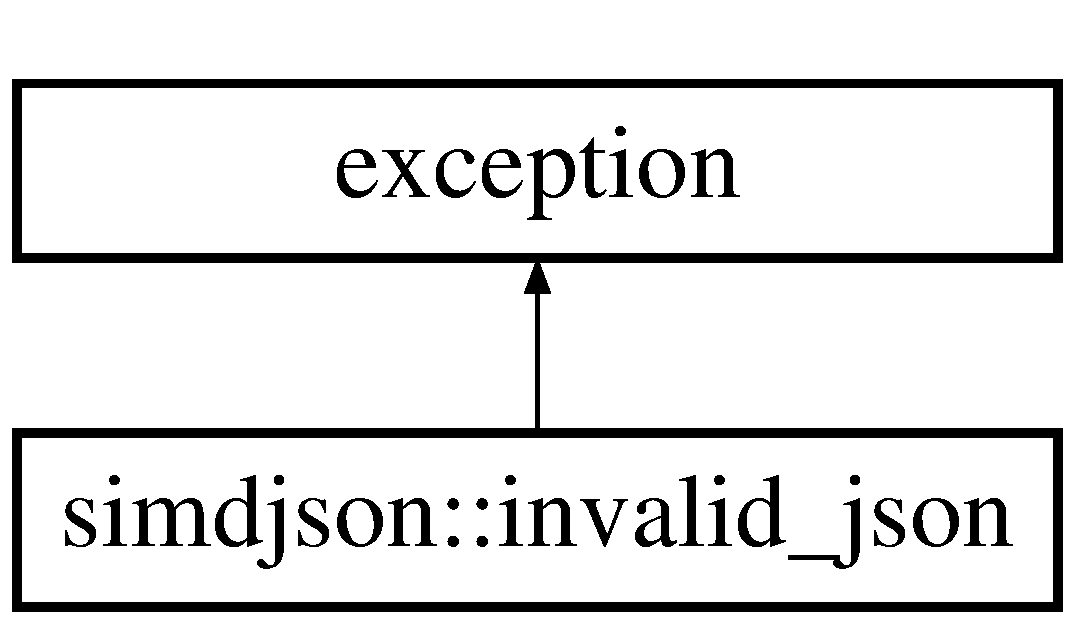
\includegraphics[height=2.000000cm]{structsimdjson_1_1invalid__json}
\end{center}
\end{figure}
\subsection*{Public Member Functions}
\begin{DoxyCompactItemize}
\item 
\mbox{\Hypertarget{structsimdjson_1_1invalid__json_a73610360ef5d59c4649db523df630667}\label{structsimdjson_1_1invalid__json_a73610360ef5d59c4649db523df630667}} 
{\bfseries invalid\+\_\+json} (\hyperlink{namespacesimdjson_a7b735a3a50ba79e3f7f14df5f77d8da9}{error\+\_\+code} \+\_\+error)
\item 
\mbox{\Hypertarget{structsimdjson_1_1invalid__json_a87689a3b8e2e23f6e23a498d0db51392}\label{structsimdjson_1_1invalid__json_a87689a3b8e2e23f6e23a498d0db51392}} 
const char $\ast$ {\bfseries what} () const noexcept
\end{DoxyCompactItemize}
\subsection*{Public Attributes}
\begin{DoxyCompactItemize}
\item 
\mbox{\Hypertarget{structsimdjson_1_1invalid__json_a06299213e2add462c0fdc7224e21bbe1}\label{structsimdjson_1_1invalid__json_a06299213e2add462c0fdc7224e21bbe1}} 
\hyperlink{namespacesimdjson_a7b735a3a50ba79e3f7f14df5f77d8da9}{error\+\_\+code} {\bfseries error}
\end{DoxyCompactItemize}


\subsection{Detailed Description}
An exception during simdjson execution. 



Definition at line 38 of file error.\+h.



The documentation for this struct was generated from the following file\+:\begin{DoxyCompactItemize}
\item 
include/simdjson/error.\+h\end{DoxyCompactItemize}

\hypertarget{classsimdjson_1_1document_1_1array_1_1iterator}{}\section{simdjson\+:\+:document\+:\+:array\+:\+:iterator Class Reference}
\label{classsimdjson_1_1document_1_1array_1_1iterator}\index{simdjson\+::document\+::array\+::iterator@{simdjson\+::document\+::array\+::iterator}}


Inherits simdjson\+::document\+::tape\+\_\+ref.

\subsection*{Public Member Functions}
\begin{DoxyCompactItemize}
\item 
\mbox{\Hypertarget{classsimdjson_1_1document_1_1array_1_1iterator_a42bad0e3e35ecd7d1fc0c96bf7263978}\label{classsimdjson_1_1document_1_1array_1_1iterator_a42bad0e3e35ecd7d1fc0c96bf7263978}} 
\hyperlink{classsimdjson_1_1document_1_1element}{element} \hyperlink{classsimdjson_1_1document_1_1array_1_1iterator_a42bad0e3e35ecd7d1fc0c96bf7263978}{operator$\ast$} () const noexcept
\begin{DoxyCompactList}\small\item\em Get the actual value. \end{DoxyCompactList}\item 
void \hyperlink{classsimdjson_1_1document_1_1array_1_1iterator_aa8458eb6195491a692a9fae5ca2508df}{operator++} () noexcept
\begin{DoxyCompactList}\small\item\em Get the next value. \end{DoxyCompactList}\item 
bool \hyperlink{classsimdjson_1_1document_1_1array_1_1iterator_a5cac863b65e9fc607d5ed7e5e2a2f35d}{operator!=} (const \hyperlink{classsimdjson_1_1document_1_1array_1_1iterator}{iterator} \&other) const noexcept
\begin{DoxyCompactList}\small\item\em Check if these values come from the same place in the J\+S\+ON. \end{DoxyCompactList}\end{DoxyCompactItemize}


\subsection{Detailed Description}


Definition at line 571 of file document.\+h.



\subsection{Member Function Documentation}
\mbox{\Hypertarget{classsimdjson_1_1document_1_1array_1_1iterator_a5cac863b65e9fc607d5ed7e5e2a2f35d}\label{classsimdjson_1_1document_1_1array_1_1iterator_a5cac863b65e9fc607d5ed7e5e2a2f35d}} 
\index{simdjson\+::document\+::array\+::iterator@{simdjson\+::document\+::array\+::iterator}!operator"!=@{operator"!=}}
\index{operator"!=@{operator"!=}!simdjson\+::document\+::array\+::iterator@{simdjson\+::document\+::array\+::iterator}}
\subsubsection{\texorpdfstring{operator"!=()}{operator!=()}}
{\footnotesize\ttfamily bool simdjson\+::document\+::array\+::iterator\+::operator!= (\begin{DoxyParamCaption}\item[{const \hyperlink{classsimdjson_1_1document_1_1array_1_1iterator}{iterator} \&}]{other }\end{DoxyParamCaption}) const\hspace{0.3cm}{\ttfamily [inline]}, {\ttfamily [noexcept]}}



Check if these values come from the same place in the J\+S\+ON. 

Part of the std\+::iterator interface. 

Definition at line 480 of file document.\+h.


\begin{DoxyCode}
480                                                                                                \{
481   \textcolor{keywordflow}{return} json\_index != other.json\_index;
482 \}
\end{DoxyCode}
\mbox{\Hypertarget{classsimdjson_1_1document_1_1array_1_1iterator_aa8458eb6195491a692a9fae5ca2508df}\label{classsimdjson_1_1document_1_1array_1_1iterator_aa8458eb6195491a692a9fae5ca2508df}} 
\index{simdjson\+::document\+::array\+::iterator@{simdjson\+::document\+::array\+::iterator}!operator++@{operator++}}
\index{operator++@{operator++}!simdjson\+::document\+::array\+::iterator@{simdjson\+::document\+::array\+::iterator}}
\subsubsection{\texorpdfstring{operator++()}{operator++()}}
{\footnotesize\ttfamily void simdjson\+::document\+::array\+::iterator\+::operator++ (\begin{DoxyParamCaption}{ }\end{DoxyParamCaption})\hspace{0.3cm}{\ttfamily [inline]}, {\ttfamily [noexcept]}}



Get the next value. 

Part of the std\+::iterator interface. 

Definition at line 483 of file document.\+h.


\begin{DoxyCode}
483                                                        \{
484   json\_index = after\_element();
485 \}
\end{DoxyCode}


The documentation for this class was generated from the following file\+:\begin{DoxyCompactItemize}
\item 
include/simdjson/document.\+h\end{DoxyCompactItemize}

\hypertarget{classsimdjson_1_1document_1_1object_1_1iterator}{}\section{simdjson\+:\+:document\+:\+:object\+:\+:iterator Class Reference}
\label{classsimdjson_1_1document_1_1object_1_1iterator}\index{simdjson\+::document\+::object\+::iterator@{simdjson\+::document\+::object\+::iterator}}


Inherits simdjson\+::document\+::tape\+\_\+ref.

\subsection*{Public Member Functions}
\begin{DoxyCompactItemize}
\item 
\mbox{\Hypertarget{classsimdjson_1_1document_1_1object_1_1iterator_a79de34f122872f0075c9d27cd7a820c5}\label{classsimdjson_1_1document_1_1object_1_1iterator_a79de34f122872f0075c9d27cd7a820c5}} 
const \hyperlink{classsimdjson_1_1document_1_1key__value__pair}{document\+::key\+\_\+value\+\_\+pair} \hyperlink{classsimdjson_1_1document_1_1object_1_1iterator_a79de34f122872f0075c9d27cd7a820c5}{operator$\ast$} () const noexcept
\begin{DoxyCompactList}\small\item\em Get the actual key/value pair. \end{DoxyCompactList}\item 
void \hyperlink{classsimdjson_1_1document_1_1object_1_1iterator_a1a97b083023759d347a0bf103a6c0d10}{operator++} () noexcept
\begin{DoxyCompactList}\small\item\em Get the next key/value pair. \end{DoxyCompactList}\item 
bool \hyperlink{classsimdjson_1_1document_1_1object_1_1iterator_ad6cbc90bf14e9d0258cea88666f8e649}{operator!=} (const \hyperlink{classsimdjson_1_1document_1_1object_1_1iterator}{iterator} \&other) const noexcept
\begin{DoxyCompactList}\small\item\em Check if these key value pairs come from the same place in the J\+S\+ON. \end{DoxyCompactList}\item 
\mbox{\Hypertarget{classsimdjson_1_1document_1_1object_1_1iterator_a7a012a54e058dd30fc53488f4efb0a13}\label{classsimdjson_1_1document_1_1object_1_1iterator_a7a012a54e058dd30fc53488f4efb0a13}} 
std\+::string\+\_\+view \hyperlink{classsimdjson_1_1document_1_1object_1_1iterator_a7a012a54e058dd30fc53488f4efb0a13}{key} () const noexcept
\begin{DoxyCompactList}\small\item\em Get the key of this key/value pair. \end{DoxyCompactList}\item 
\mbox{\Hypertarget{classsimdjson_1_1document_1_1object_1_1iterator_a8c8e43efcc7b589f9d6e73e338617257}\label{classsimdjson_1_1document_1_1object_1_1iterator_a8c8e43efcc7b589f9d6e73e338617257}} 
const char $\ast$ \hyperlink{classsimdjson_1_1document_1_1object_1_1iterator_a8c8e43efcc7b589f9d6e73e338617257}{key\+\_\+c\+\_\+str} () const noexcept
\begin{DoxyCompactList}\small\item\em Get the key of this key/value pair. \end{DoxyCompactList}\item 
\mbox{\Hypertarget{classsimdjson_1_1document_1_1object_1_1iterator_a267ad9db1110a62ad19e8031c88f31de}\label{classsimdjson_1_1document_1_1object_1_1iterator_a267ad9db1110a62ad19e8031c88f31de}} 
\hyperlink{classsimdjson_1_1document_1_1element}{element} \hyperlink{classsimdjson_1_1document_1_1object_1_1iterator_a267ad9db1110a62ad19e8031c88f31de}{value} () const noexcept
\begin{DoxyCompactList}\small\item\em Get the value of this key/value pair. \end{DoxyCompactList}\end{DoxyCompactItemize}


\subsection{Detailed Description}


Definition at line 620 of file document.\+h.



\subsection{Member Function Documentation}
\mbox{\Hypertarget{classsimdjson_1_1document_1_1object_1_1iterator_ad6cbc90bf14e9d0258cea88666f8e649}\label{classsimdjson_1_1document_1_1object_1_1iterator_ad6cbc90bf14e9d0258cea88666f8e649}} 
\index{simdjson\+::document\+::object\+::iterator@{simdjson\+::document\+::object\+::iterator}!operator"!=@{operator"!=}}
\index{operator"!=@{operator"!=}!simdjson\+::document\+::object\+::iterator@{simdjson\+::document\+::object\+::iterator}}
\subsubsection{\texorpdfstring{operator"!=()}{operator!=()}}
{\footnotesize\ttfamily bool simdjson\+::document\+::object\+::iterator\+::operator!= (\begin{DoxyParamCaption}\item[{const \hyperlink{classsimdjson_1_1document_1_1object_1_1iterator}{iterator} \&}]{other }\end{DoxyParamCaption}) const\hspace{0.3cm}{\ttfamily [inline]}, {\ttfamily [noexcept]}}



Check if these key value pairs come from the same place in the J\+S\+ON. 

Part of the std\+::iterator interface. 

Definition at line 524 of file document.\+h.


\begin{DoxyCode}
524                                                                                                  \{
525   \textcolor{keywordflow}{return} json\_index != other.json\_index;
526 \}
\end{DoxyCode}
\mbox{\Hypertarget{classsimdjson_1_1document_1_1object_1_1iterator_a1a97b083023759d347a0bf103a6c0d10}\label{classsimdjson_1_1document_1_1object_1_1iterator_a1a97b083023759d347a0bf103a6c0d10}} 
\index{simdjson\+::document\+::object\+::iterator@{simdjson\+::document\+::object\+::iterator}!operator++@{operator++}}
\index{operator++@{operator++}!simdjson\+::document\+::object\+::iterator@{simdjson\+::document\+::object\+::iterator}}
\subsubsection{\texorpdfstring{operator++()}{operator++()}}
{\footnotesize\ttfamily void simdjson\+::document\+::object\+::iterator\+::operator++ (\begin{DoxyParamCaption}{ }\end{DoxyParamCaption})\hspace{0.3cm}{\ttfamily [inline]}, {\ttfamily [noexcept]}}



Get the next key/value pair. 

Part of the std\+::iterator interface. 

Definition at line 527 of file document.\+h.


\begin{DoxyCode}
527                                                         \{
528   json\_index++;
529   json\_index = after\_element();
530 \}
\end{DoxyCode}


The documentation for this class was generated from the following file\+:\begin{DoxyCompactItemize}
\item 
include/simdjson/document.\+h\end{DoxyCompactItemize}

\hypertarget{classsimdjson_1_1_json_stream}{}\section{simdjson\+:\+:Json\+Stream$<$ string\+\_\+container $>$ Class Template Reference}
\label{classsimdjson_1_1_json_stream}\index{simdjson\+::\+Json\+Stream$<$ string\+\_\+container $>$@{simdjson\+::\+Json\+Stream$<$ string\+\_\+container $>$}}


The template parameter (string\+\_\+container) must support the data() and size() methods, returning a pointer to a char$\ast$ and to the number of bytes respectively.  




{\ttfamily \#include $<$jsonstream.\+h$>$}

\subsection*{Public Member Functions}
\begin{DoxyCompactItemize}
\item 
\hyperlink{classsimdjson_1_1_json_stream_ac7ab1f7dd9d839e155f32aa70ca3826d}{Json\+Stream} (const string\+\_\+container \&s, size\+\_\+t batch\+\_\+size=1000000)
\begin{DoxyCompactList}\small\item\em Create a \hyperlink{classsimdjson_1_1_json_stream}{Json\+Stream} object that can be used to parse sequentially the valid J\+S\+ON documents found in the buffer \char`\"{}buf\char`\"{}. \end{DoxyCompactList}\item 
\mbox{\Hypertarget{classsimdjson_1_1_json_stream_ab386509a4a926e325e90bab1b5a96e5e}\label{classsimdjson_1_1_json_stream_ab386509a4a926e325e90bab1b5a96e5e}} 
int {\bfseries json\+\_\+parse} (\hyperlink{classsimdjson_1_1document_1_1parser}{document\+::parser} \&parser)
\item 
size\+\_\+t \hyperlink{classsimdjson_1_1_json_stream_a01493e28b0606bcef1e03c233214382b}{get\+\_\+current\+\_\+buffer\+\_\+loc} () const
\begin{DoxyCompactList}\small\item\em Returns the location (index) of where the next document should be in the buffer. \end{DoxyCompactList}\item 
size\+\_\+t \hyperlink{classsimdjson_1_1_json_stream_a160e592d44374cc21c12a58a1648196b}{get\+\_\+n\+\_\+parsed\+\_\+docs} () const
\begin{DoxyCompactList}\small\item\em Returns the total amount of complete documents parsed by the \hyperlink{classsimdjson_1_1_json_stream}{Json\+Stream}, in the current buffer, at the given time. \end{DoxyCompactList}\item 
size\+\_\+t \hyperlink{classsimdjson_1_1_json_stream_ac63006b60b0446cd20dfc102131e8a98}{get\+\_\+n\+\_\+bytes\+\_\+parsed} () const
\begin{DoxyCompactList}\small\item\em Returns the total amount of data (in bytes) parsed by the \hyperlink{classsimdjson_1_1_json_stream}{Json\+Stream}, in the current buffer, at the given time. \end{DoxyCompactList}\end{DoxyCompactItemize}


\subsection{Detailed Description}
\subsubsection*{template$<$class string\+\_\+container = padded\+\_\+string$>$\newline
class simdjson\+::\+Json\+Stream$<$ string\+\_\+container $>$}

The template parameter (string\+\_\+container) must support the data() and size() methods, returning a pointer to a char$\ast$ and to the number of bytes respectively. 

The simdjson parser may read up to S\+I\+M\+D\+J\+S\+O\+N\+\_\+\+P\+A\+D\+D\+I\+NG bytes beyond the end of the string, so if you do not use a \hyperlink{structsimdjson_1_1padded__string}{padded\+\_\+string} container, you have the responsability to overallocated. If you fail to do so, your software may crash if you cross a page boundary, and you should expect memory checkers to object. Most users should use a \hyperlink{structsimdjson_1_1padded__string}{simdjson\+::padded\+\_\+string}. 

Definition at line 53 of file jsonstream.\+h.



\subsection{Constructor \& Destructor Documentation}
\mbox{\Hypertarget{classsimdjson_1_1_json_stream_ac7ab1f7dd9d839e155f32aa70ca3826d}\label{classsimdjson_1_1_json_stream_ac7ab1f7dd9d839e155f32aa70ca3826d}} 
\index{simdjson\+::\+Json\+Stream@{simdjson\+::\+Json\+Stream}!Json\+Stream@{Json\+Stream}}
\index{Json\+Stream@{Json\+Stream}!simdjson\+::\+Json\+Stream@{simdjson\+::\+Json\+Stream}}
\subsubsection{\texorpdfstring{Json\+Stream()}{JsonStream()}}
{\footnotesize\ttfamily template$<$class string\+\_\+container $>$ \\
\hyperlink{classsimdjson_1_1_json_stream}{simdjson\+::\+Json\+Stream}$<$ string\+\_\+container $>$\+::\hyperlink{classsimdjson_1_1_json_stream}{Json\+Stream} (\begin{DoxyParamCaption}\item[{const string\+\_\+container \&}]{s,  }\item[{size\+\_\+t}]{batch\+\_\+size = {\ttfamily 1000000} }\end{DoxyParamCaption})}



Create a \hyperlink{classsimdjson_1_1_json_stream}{Json\+Stream} object that can be used to parse sequentially the valid J\+S\+ON documents found in the buffer \char`\"{}buf\char`\"{}. 

The batch\+\_\+size must be at least as large as the biggest document in the file, but not too large to submerge the cached memory. We found that 1\+MB is somewhat a sweet spot for now.

The user is expected to call the following json\+\_\+parse method to parse the next valid J\+S\+ON document found in the buffer. This method can and is expected to be called in a loop.

Various methods are offered to keep track of the status, like get\+\_\+current\+\_\+buffer\+\_\+loc, get\+\_\+n\+\_\+parsed\+\_\+docs, get\+\_\+n\+\_\+bytes\+\_\+parsed, etc. 

Definition at line 226 of file jsonstream.\+h.


\begin{DoxyCode}
228     : str(s), \_batch\_size(batchSize) \{
229 \}
\end{DoxyCode}


\subsection{Member Function Documentation}
\mbox{\Hypertarget{classsimdjson_1_1_json_stream_a01493e28b0606bcef1e03c233214382b}\label{classsimdjson_1_1_json_stream_a01493e28b0606bcef1e03c233214382b}} 
\index{simdjson\+::\+Json\+Stream@{simdjson\+::\+Json\+Stream}!get\+\_\+current\+\_\+buffer\+\_\+loc@{get\+\_\+current\+\_\+buffer\+\_\+loc}}
\index{get\+\_\+current\+\_\+buffer\+\_\+loc@{get\+\_\+current\+\_\+buffer\+\_\+loc}!simdjson\+::\+Json\+Stream@{simdjson\+::\+Json\+Stream}}
\subsubsection{\texorpdfstring{get\+\_\+current\+\_\+buffer\+\_\+loc()}{get\_current\_buffer\_loc()}}
{\footnotesize\ttfamily template$<$class string\+\_\+container  = padded\+\_\+string$>$ \\
size\+\_\+t \hyperlink{classsimdjson_1_1_json_stream}{simdjson\+::\+Json\+Stream}$<$ string\+\_\+container $>$\+::get\+\_\+current\+\_\+buffer\+\_\+loc (\begin{DoxyParamCaption}{ }\end{DoxyParamCaption}) const\hspace{0.3cm}{\ttfamily [inline]}}



Returns the location (index) of where the next document should be in the buffer. 

Can be used for debugging, it tells the user the position of the end of the last valid J\+S\+ON document parsed 

Definition at line 117 of file jsonstream.\+h.


\begin{DoxyCode}
117 \{ \textcolor{keywordflow}{return} current\_buffer\_loc; \}
\end{DoxyCode}
\mbox{\Hypertarget{classsimdjson_1_1_json_stream_ac63006b60b0446cd20dfc102131e8a98}\label{classsimdjson_1_1_json_stream_ac63006b60b0446cd20dfc102131e8a98}} 
\index{simdjson\+::\+Json\+Stream@{simdjson\+::\+Json\+Stream}!get\+\_\+n\+\_\+bytes\+\_\+parsed@{get\+\_\+n\+\_\+bytes\+\_\+parsed}}
\index{get\+\_\+n\+\_\+bytes\+\_\+parsed@{get\+\_\+n\+\_\+bytes\+\_\+parsed}!simdjson\+::\+Json\+Stream@{simdjson\+::\+Json\+Stream}}
\subsubsection{\texorpdfstring{get\+\_\+n\+\_\+bytes\+\_\+parsed()}{get\_n\_bytes\_parsed()}}
{\footnotesize\ttfamily template$<$class string\+\_\+container  = padded\+\_\+string$>$ \\
size\+\_\+t \hyperlink{classsimdjson_1_1_json_stream}{simdjson\+::\+Json\+Stream}$<$ string\+\_\+container $>$\+::get\+\_\+n\+\_\+bytes\+\_\+parsed (\begin{DoxyParamCaption}{ }\end{DoxyParamCaption}) const\hspace{0.3cm}{\ttfamily [inline]}}



Returns the total amount of data (in bytes) parsed by the \hyperlink{classsimdjson_1_1_json_stream}{Json\+Stream}, in the current buffer, at the given time. 



Definition at line 125 of file jsonstream.\+h.


\begin{DoxyCode}
125 \{ \textcolor{keywordflow}{return} n\_bytes\_parsed; \}
\end{DoxyCode}
\mbox{\Hypertarget{classsimdjson_1_1_json_stream_a160e592d44374cc21c12a58a1648196b}\label{classsimdjson_1_1_json_stream_a160e592d44374cc21c12a58a1648196b}} 
\index{simdjson\+::\+Json\+Stream@{simdjson\+::\+Json\+Stream}!get\+\_\+n\+\_\+parsed\+\_\+docs@{get\+\_\+n\+\_\+parsed\+\_\+docs}}
\index{get\+\_\+n\+\_\+parsed\+\_\+docs@{get\+\_\+n\+\_\+parsed\+\_\+docs}!simdjson\+::\+Json\+Stream@{simdjson\+::\+Json\+Stream}}
\subsubsection{\texorpdfstring{get\+\_\+n\+\_\+parsed\+\_\+docs()}{get\_n\_parsed\_docs()}}
{\footnotesize\ttfamily template$<$class string\+\_\+container  = padded\+\_\+string$>$ \\
size\+\_\+t \hyperlink{classsimdjson_1_1_json_stream}{simdjson\+::\+Json\+Stream}$<$ string\+\_\+container $>$\+::get\+\_\+n\+\_\+parsed\+\_\+docs (\begin{DoxyParamCaption}{ }\end{DoxyParamCaption}) const\hspace{0.3cm}{\ttfamily [inline]}}



Returns the total amount of complete documents parsed by the \hyperlink{classsimdjson_1_1_json_stream}{Json\+Stream}, in the current buffer, at the given time. 



Definition at line 121 of file jsonstream.\+h.


\begin{DoxyCode}
121 \{ \textcolor{keywordflow}{return} n\_parsed\_docs; \}
\end{DoxyCode}


The documentation for this class was generated from the following file\+:\begin{DoxyCompactItemize}
\item 
include/simdjson/jsonstream.\+h\end{DoxyCompactItemize}

\hypertarget{classsimdjson_1_1document_1_1key__value__pair}{}\section{simdjson\+:\+:document\+:\+:key\+\_\+value\+\_\+pair Class Reference}
\label{classsimdjson_1_1document_1_1key__value__pair}\index{simdjson\+::document\+::key\+\_\+value\+\_\+pair@{simdjson\+::document\+::key\+\_\+value\+\_\+pair}}


Key/value pair in an object.  




{\ttfamily \#include $<$document.\+h$>$}

\subsection*{Public Attributes}
\begin{DoxyCompactItemize}
\item 
\mbox{\Hypertarget{classsimdjson_1_1document_1_1key__value__pair_a9c35a679f02d7feb2913c760fdec33d7}\label{classsimdjson_1_1document_1_1key__value__pair_a9c35a679f02d7feb2913c760fdec33d7}} 
std\+::string\+\_\+view {\bfseries key}
\item 
\mbox{\Hypertarget{classsimdjson_1_1document_1_1key__value__pair_a75a8ddcb41eb04179a500f9c65a11e20}\label{classsimdjson_1_1document_1_1key__value__pair_a75a8ddcb41eb04179a500f9c65a11e20}} 
\hyperlink{classsimdjson_1_1document_1_1element}{document\+::element} {\bfseries value}
\end{DoxyCompactItemize}


\subsection{Detailed Description}
Key/value pair in an object. 

Definition at line 704 of file document.\+h.



The documentation for this class was generated from the following file\+:\begin{DoxyCompactItemize}
\item 
include/simdjson/document.\+h\end{DoxyCompactItemize}

\hypertarget{classsimdjson_1_1document_1_1object}{}\section{simdjson\+:\+:document\+:\+:object Class Reference}
\label{classsimdjson_1_1document_1_1object}\index{simdjson\+::document\+::object@{simdjson\+::document\+::object}}


Represents a J\+S\+ON object.  




{\ttfamily \#include $<$document.\+h$>$}



Inherits simdjson\+::document\+::tape\+\_\+ref.

\subsection*{Classes}
\begin{DoxyCompactItemize}
\item 
class \hyperlink{classsimdjson_1_1document_1_1object_1_1iterator}{iterator}
\end{DoxyCompactItemize}
\subsection*{Public Member Functions}
\begin{DoxyCompactItemize}
\item 
\hyperlink{classsimdjson_1_1document_1_1object_1_1iterator}{iterator} \hyperlink{classsimdjson_1_1document_1_1object_a88e638207141099532b524a8814540e0}{begin} () const noexcept
\begin{DoxyCompactList}\small\item\em Return the first key/value pair. \end{DoxyCompactList}\item 
\hyperlink{classsimdjson_1_1document_1_1object_1_1iterator}{iterator} \hyperlink{classsimdjson_1_1document_1_1object_a38ab9979d9eecb0b70768dcde9d12864}{end} () const noexcept
\begin{DoxyCompactList}\small\item\em One past the last key/value pair. \end{DoxyCompactList}\item 
\hyperlink{classsimdjson_1_1document_1_1element__result}{element\+\_\+result}$<$ \hyperlink{classsimdjson_1_1document_1_1element}{element} $>$ \hyperlink{classsimdjson_1_1document_1_1object_a5b52e82f66a45fb9a669a643aabf60ae}{operator\mbox{[}$\,$\mbox{]}} (const std\+::string\+\_\+view \&s) const noexcept
\begin{DoxyCompactList}\small\item\em Get the value associated with the given key. \end{DoxyCompactList}\item 
\hyperlink{classsimdjson_1_1document_1_1element__result}{element\+\_\+result}$<$ \hyperlink{classsimdjson_1_1document_1_1element}{element} $>$ \hyperlink{classsimdjson_1_1document_1_1object_a57e850feb7121e097754e5e82a5de2a4}{operator\mbox{[}$\,$\mbox{]}} (const char $\ast$s) const noexcept
\begin{DoxyCompactList}\small\item\em Get the value associated with the given key. \end{DoxyCompactList}\end{DoxyCompactItemize}


\subsection{Detailed Description}
Represents a J\+S\+ON object. 

Definition at line 618 of file document.\+h.



\subsection{Member Function Documentation}
\mbox{\Hypertarget{classsimdjson_1_1document_1_1object_a88e638207141099532b524a8814540e0}\label{classsimdjson_1_1document_1_1object_a88e638207141099532b524a8814540e0}} 
\index{simdjson\+::document\+::object@{simdjson\+::document\+::object}!begin@{begin}}
\index{begin@{begin}!simdjson\+::document\+::object@{simdjson\+::document\+::object}}
\subsubsection{\texorpdfstring{begin()}{begin()}}
{\footnotesize\ttfamily \hyperlink{classsimdjson_1_1document_1_1object_1_1iterator}{document\+::object\+::iterator} simdjson\+::document\+::object\+::begin (\begin{DoxyParamCaption}{ }\end{DoxyParamCaption}) const\hspace{0.3cm}{\ttfamily [inline]}, {\ttfamily [noexcept]}}



Return the first key/value pair. 

Part of the std\+::iterable interface. 

Definition at line 492 of file document.\+h.


\begin{DoxyCode}
492                                                                    \{
493   \textcolor{keywordflow}{return} iterator(doc, json\_index + 1);
494 \}
\end{DoxyCode}
\mbox{\Hypertarget{classsimdjson_1_1document_1_1object_a38ab9979d9eecb0b70768dcde9d12864}\label{classsimdjson_1_1document_1_1object_a38ab9979d9eecb0b70768dcde9d12864}} 
\index{simdjson\+::document\+::object@{simdjson\+::document\+::object}!end@{end}}
\index{end@{end}!simdjson\+::document\+::object@{simdjson\+::document\+::object}}
\subsubsection{\texorpdfstring{end()}{end()}}
{\footnotesize\ttfamily \hyperlink{classsimdjson_1_1document_1_1object_1_1iterator}{document\+::object\+::iterator} simdjson\+::document\+::object\+::end (\begin{DoxyParamCaption}{ }\end{DoxyParamCaption}) const\hspace{0.3cm}{\ttfamily [inline]}, {\ttfamily [noexcept]}}



One past the last key/value pair. 

Part of the std\+::iterable interface. 

Definition at line 495 of file document.\+h.


\begin{DoxyCode}
495                                                                  \{
496   \textcolor{keywordflow}{return} iterator(doc, after\_element() - 1);
497 \}
\end{DoxyCode}
\mbox{\Hypertarget{classsimdjson_1_1document_1_1object_a5b52e82f66a45fb9a669a643aabf60ae}\label{classsimdjson_1_1document_1_1object_a5b52e82f66a45fb9a669a643aabf60ae}} 
\index{simdjson\+::document\+::object@{simdjson\+::document\+::object}!operator\mbox{[}\mbox{]}@{operator[]}}
\index{operator\mbox{[}\mbox{]}@{operator[]}!simdjson\+::document\+::object@{simdjson\+::document\+::object}}
\subsubsection{\texorpdfstring{operator[]()}{operator[]()}\hspace{0.1cm}{\footnotesize\ttfamily [1/2]}}
{\footnotesize\ttfamily \hyperlink{classsimdjson_1_1document_1_1element__result}{document\+::element\+\_\+result}$<$ \hyperlink{classsimdjson_1_1document_1_1element}{document\+::element} $>$ simdjson\+::document\+::object\+::operator\mbox{[}$\,$\mbox{]} (\begin{DoxyParamCaption}\item[{const std\+::string\+\_\+view \&}]{s }\end{DoxyParamCaption}) const\hspace{0.3cm}{\ttfamily [inline]}, {\ttfamily [noexcept]}}



Get the value associated with the given key. 

The key will be matched against {\bfseries unescaped} J\+S\+ON\+:

\hyperlink{classsimdjson_1_1document_a6f11cda7c4a06fffdc00fdc97d98ae2b}{document\+::parse}(R\char`\"{}(\{ \char`\"{}a~\newline
\char`\"{}\+: 1 \})\char`\"{})\mbox{[}\char`\"{}a\textbackslash{}n\char`\"{}\mbox{]}.as\+\_\+uint64\+\_\+t().value == 1 \hyperlink{classsimdjson_1_1document_a6f11cda7c4a06fffdc00fdc97d98ae2b}{document\+::parse}(R\char`\"{}(\{ \char`\"{}a~\newline
\char`\"{}\+: 1 \})\char`\"{})\mbox{[}\char`\"{}a\textbackslash{}\textbackslash{}n\char`\"{}\mbox{]}.as\+\_\+uint64\+\_\+t().error == N\+O\+\_\+\+S\+U\+C\+H\+\_\+\+F\+I\+E\+LD

\begin{DoxyReturn}{Returns}
The value associated with this field, or\+:
\begin{DoxyItemize}
\item N\+O\+\_\+\+S\+U\+C\+H\+\_\+\+F\+I\+E\+LD if the field does not exist in the object 
\end{DoxyItemize}
\end{DoxyReturn}


Definition at line 498 of file document.\+h.


\begin{DoxyCode}
498                                                                                                            
             \{
499   iterator end\_field = \hyperlink{classsimdjson_1_1document_1_1object_a38ab9979d9eecb0b70768dcde9d12864}{end}();
500   \textcolor{keywordflow}{for} (iterator field = \hyperlink{classsimdjson_1_1document_1_1object_a88e638207141099532b524a8814540e0}{begin}(); field != end\_field; ++field) \{
501     \textcolor{keywordflow}{if} (key == field.key()) \{
502       \textcolor{keywordflow}{return} field.value();
503     \}
504   \}
505   \textcolor{keywordflow}{return} NO\_SUCH\_FIELD;
506 \}
\end{DoxyCode}
\mbox{\Hypertarget{classsimdjson_1_1document_1_1object_a57e850feb7121e097754e5e82a5de2a4}\label{classsimdjson_1_1document_1_1object_a57e850feb7121e097754e5e82a5de2a4}} 
\index{simdjson\+::document\+::object@{simdjson\+::document\+::object}!operator\mbox{[}\mbox{]}@{operator[]}}
\index{operator\mbox{[}\mbox{]}@{operator[]}!simdjson\+::document\+::object@{simdjson\+::document\+::object}}
\subsubsection{\texorpdfstring{operator[]()}{operator[]()}\hspace{0.1cm}{\footnotesize\ttfamily [2/2]}}
{\footnotesize\ttfamily \hyperlink{classsimdjson_1_1document_1_1element__result}{document\+::element\+\_\+result}$<$ \hyperlink{classsimdjson_1_1document_1_1element}{document\+::element} $>$ simdjson\+::document\+::object\+::operator\mbox{[}$\,$\mbox{]} (\begin{DoxyParamCaption}\item[{const char $\ast$}]{s }\end{DoxyParamCaption}) const\hspace{0.3cm}{\ttfamily [inline]}, {\ttfamily [noexcept]}}



Get the value associated with the given key. 

Note\+: The key will be matched against {\bfseries unescaped} J\+S\+ON\+:

\hyperlink{classsimdjson_1_1document_a6f11cda7c4a06fffdc00fdc97d98ae2b}{document\+::parse}(R\char`\"{}(\{ \char`\"{}a~\newline
\char`\"{}\+: 1 \})\char`\"{})\mbox{[}\char`\"{}a\textbackslash{}n\char`\"{}\mbox{]}.as\+\_\+uint64\+\_\+t().value == 1 \hyperlink{classsimdjson_1_1document_a6f11cda7c4a06fffdc00fdc97d98ae2b}{document\+::parse}(R\char`\"{}(\{ \char`\"{}a~\newline
\char`\"{}\+: 1 \})\char`\"{})\mbox{[}\char`\"{}a\textbackslash{}\textbackslash{}n\char`\"{}\mbox{]}.as\+\_\+uint64\+\_\+t().error == N\+O\+\_\+\+S\+U\+C\+H\+\_\+\+F\+I\+E\+LD

\begin{DoxyReturn}{Returns}
The value associated with this field, or\+:
\begin{DoxyItemize}
\item N\+O\+\_\+\+S\+U\+C\+H\+\_\+\+F\+I\+E\+LD if the field does not exist in the object 
\end{DoxyItemize}
\end{DoxyReturn}


Definition at line 507 of file document.\+h.


\begin{DoxyCode}
507                                                                                                         \{
508   iterator end\_field = \hyperlink{classsimdjson_1_1document_1_1object_a38ab9979d9eecb0b70768dcde9d12864}{end}();
509   \textcolor{keywordflow}{for} (iterator field = \hyperlink{classsimdjson_1_1document_1_1object_a88e638207141099532b524a8814540e0}{begin}(); field != end\_field; ++field) \{
510     \textcolor{keywordflow}{if} (!strcmp(key, field.key\_c\_str())) \{
511       \textcolor{keywordflow}{return} field.value();
512     \}
513   \}
514   \textcolor{keywordflow}{return} NO\_SUCH\_FIELD;
515 \}
\end{DoxyCode}


The documentation for this class was generated from the following file\+:\begin{DoxyCompactItemize}
\item 
include/simdjson/document.\+h\end{DoxyCompactItemize}

\hypertarget{structsimdjson_1_1padded__string}{}\section{simdjson\+:\+:padded\+\_\+string Struct Reference}
\label{structsimdjson_1_1padded__string}\index{simdjson\+::padded\+\_\+string@{simdjson\+::padded\+\_\+string}}
\subsection*{Public Member Functions}
\begin{DoxyCompactItemize}
\item 
\mbox{\Hypertarget{structsimdjson_1_1padded__string_ac06ec74c78934565cdf50df163d35476}\label{structsimdjson_1_1padded__string_ac06ec74c78934565cdf50df163d35476}} 
{\bfseries padded\+\_\+string} (size\+\_\+t length) noexcept
\item 
\mbox{\Hypertarget{structsimdjson_1_1padded__string_a1b15f9345c0215e7548df1aa0105de98}\label{structsimdjson_1_1padded__string_a1b15f9345c0215e7548df1aa0105de98}} 
{\bfseries padded\+\_\+string} (const char $\ast$data, size\+\_\+t length) noexcept
\item 
\mbox{\Hypertarget{structsimdjson_1_1padded__string_a44fb0f219f05528e606f79dab7c32482}\label{structsimdjson_1_1padded__string_a44fb0f219f05528e606f79dab7c32482}} 
{\bfseries padded\+\_\+string} (const std\+::string \&str\+\_\+) noexcept
\item 
\mbox{\Hypertarget{structsimdjson_1_1padded__string_a6199f5bf259fcac114addeef569cf5a5}\label{structsimdjson_1_1padded__string_a6199f5bf259fcac114addeef569cf5a5}} 
{\bfseries padded\+\_\+string} (std\+::string\+\_\+view sv\+\_\+) noexcept
\item 
\mbox{\Hypertarget{structsimdjson_1_1padded__string_a952eaf7ff8ddf252d9c00a693978a4da}\label{structsimdjson_1_1padded__string_a952eaf7ff8ddf252d9c00a693978a4da}} 
{\bfseries padded\+\_\+string} (\hyperlink{structsimdjson_1_1padded__string}{padded\+\_\+string} \&\&o) noexcept
\item 
\mbox{\Hypertarget{structsimdjson_1_1padded__string_a84b0bcaa338d89a2bb0d44b8dfa48db6}\label{structsimdjson_1_1padded__string_a84b0bcaa338d89a2bb0d44b8dfa48db6}} 
\hyperlink{structsimdjson_1_1padded__string}{padded\+\_\+string} \& {\bfseries operator=} (\hyperlink{structsimdjson_1_1padded__string}{padded\+\_\+string} \&\&o)
\item 
\mbox{\Hypertarget{structsimdjson_1_1padded__string_a345beaab26aa96824e13d4294819dc9a}\label{structsimdjson_1_1padded__string_a345beaab26aa96824e13d4294819dc9a}} 
void {\bfseries swap} (\hyperlink{structsimdjson_1_1padded__string}{padded\+\_\+string} \&o)
\item 
\mbox{\Hypertarget{structsimdjson_1_1padded__string_a4c23453d923380e8fb39b5e6289007f0}\label{structsimdjson_1_1padded__string_a4c23453d923380e8fb39b5e6289007f0}} 
size\+\_\+t {\bfseries size} () const
\item 
\mbox{\Hypertarget{structsimdjson_1_1padded__string_a998222a5edf719def1f3be73de285c9c}\label{structsimdjson_1_1padded__string_a998222a5edf719def1f3be73de285c9c}} 
size\+\_\+t {\bfseries length} () const
\item 
\mbox{\Hypertarget{structsimdjson_1_1padded__string_a981e99cf1bcd0aa0218459c8720632b5}\label{structsimdjson_1_1padded__string_a981e99cf1bcd0aa0218459c8720632b5}} 
char $\ast$ {\bfseries data} () const
\end{DoxyCompactItemize}


\subsection{Detailed Description}


Definition at line 34 of file padded\+\_\+string.\+h.



The documentation for this struct was generated from the following file\+:\begin{DoxyCompactItemize}
\item 
include/simdjson/padded\+\_\+string.\+h\end{DoxyCompactItemize}

\hypertarget{classsimdjson_1_1document_1_1parser}{}\section{simdjson\+:\+:document\+:\+:parser Class Reference}
\label{classsimdjson_1_1document_1_1parser}\index{simdjson\+::document\+::parser@{simdjson\+::document\+::parser}}


A persistent document parser.  




{\ttfamily \#include $<$document.\+h$>$}

\subsection*{Public Types}
\begin{DoxyCompactItemize}
\item 
using \hyperlink{classsimdjson_1_1document_1_1parser_af98e5ba546a37967e0bfee969d1d5f48}{Iterator} = \hyperlink{classsimdjson_1_1document__iterator}{document\+::iterator}
\item 
using \hyperlink{classsimdjson_1_1document_1_1parser_a26aa1a76e9ecf5371736aa44b5f6d74a}{Invalid\+J\+S\+ON} = \hyperlink{structsimdjson_1_1invalid__json}{invalid\+\_\+json}
\end{DoxyCompactItemize}
\subsection*{Public Member Functions}
\begin{DoxyCompactItemize}
\item 
\hyperlink{classsimdjson_1_1document_1_1parser_a656d0ad716faf5085e885581ec598466}{parser} ()=default
\begin{DoxyCompactList}\small\item\em Create a J\+S\+ON parser with zero capacity. \end{DoxyCompactList}\item 
\hyperlink{classsimdjson_1_1document_1_1parser_a01e70a75fd87c764982b9e5f4e87eddf}{$\sim$parser} ()=default
\begin{DoxyCompactList}\small\item\em Deallocate the J\+S\+ON parser. \end{DoxyCompactList}\item 
\hyperlink{classsimdjson_1_1document_1_1parser_a1996defcd55a2bded7e01308fd21ae87}{parser} (\hyperlink{classsimdjson_1_1document_1_1parser}{document\+::parser} \&\&other)=default
\begin{DoxyCompactList}\small\item\em Take another parser\textquotesingle{}s buffers and state. \end{DoxyCompactList}\item 
\hyperlink{classsimdjson_1_1document_1_1parser}{parser} \& \hyperlink{classsimdjson_1_1document_1_1parser_ab59a0096c2192266961b2d1f9f449470}{operator=} (\hyperlink{classsimdjson_1_1document_1_1parser}{document\+::parser} \&\&other)=default
\begin{DoxyCompactList}\small\item\em Take another parser\textquotesingle{}s buffers and state. \end{DoxyCompactList}\item 
\hyperlink{classsimdjson_1_1document_1_1doc__ref__result}{doc\+\_\+ref\+\_\+result} \hyperlink{classsimdjson_1_1document_1_1parser_a3eb1fd46ea0dad62eceed4b1c302b7ad}{parse} (const uint8\+\_\+t $\ast$buf, size\+\_\+t len, bool realloc\+\_\+if\+\_\+needed=true) noexcept
\begin{DoxyCompactList}\small\item\em Parse a J\+S\+ON document and return a reference to it. \end{DoxyCompactList}\item 
\hyperlink{classsimdjson_1_1document_1_1doc__ref__result}{doc\+\_\+ref\+\_\+result} \hyperlink{classsimdjson_1_1document_1_1parser_a1ce12050358a969596ced70f9786c1cc}{parse} (const char $\ast$buf, size\+\_\+t len, bool realloc\+\_\+if\+\_\+needed=true) noexcept
\begin{DoxyCompactList}\small\item\em Parse a J\+S\+ON document and return a reference to it. \end{DoxyCompactList}\item 
\hyperlink{classsimdjson_1_1document_1_1doc__ref__result}{doc\+\_\+ref\+\_\+result} \hyperlink{classsimdjson_1_1document_1_1parser_ada490fbaf30ec3df5679b86e9b6914bd}{parse} (const std\+::string \&s) noexcept
\begin{DoxyCompactList}\small\item\em Parse a J\+S\+ON document and return a reference to it. \end{DoxyCompactList}\item 
\hyperlink{classsimdjson_1_1document_1_1doc__ref__result}{doc\+\_\+ref\+\_\+result} \hyperlink{classsimdjson_1_1document_1_1parser_a5c062f8ab3f45a5cb144056dde60b993}{parse} (const \hyperlink{structsimdjson_1_1padded__string}{padded\+\_\+string} \&s) noexcept
\begin{DoxyCompactList}\small\item\em Parse a J\+S\+ON document and return a reference to it. \end{DoxyCompactList}\item 
\mbox{\Hypertarget{classsimdjson_1_1document_1_1parser_a505d0eecc82a63ffc60b6fd6a8765c48}\label{classsimdjson_1_1document_1_1parser_a505d0eecc82a63ffc60b6fd6a8765c48}} 
\hyperlink{classsimdjson_1_1document_1_1doc__ref__result}{doc\+\_\+ref\+\_\+result} {\bfseries parse} (const char $\ast$buf) noexcept=delete
\item 
\mbox{\Hypertarget{classsimdjson_1_1document_1_1parser_af9ea6b75fa9c41c6633fdcf059744cb2}\label{classsimdjson_1_1document_1_1parser_af9ea6b75fa9c41c6633fdcf059744cb2}} 
size\+\_\+t \hyperlink{classsimdjson_1_1document_1_1parser_af9ea6b75fa9c41c6633fdcf059744cb2}{capacity} ()
\begin{DoxyCompactList}\small\item\em Current capacity\+: the largest document this parser can support without reallocating. \end{DoxyCompactList}\item 
\mbox{\Hypertarget{classsimdjson_1_1document_1_1parser_ae3ccf7ff0c0aa18d6ba70d3e063461b7}\label{classsimdjson_1_1document_1_1parser_ae3ccf7ff0c0aa18d6ba70d3e063461b7}} 
size\+\_\+t \hyperlink{classsimdjson_1_1document_1_1parser_ae3ccf7ff0c0aa18d6ba70d3e063461b7}{max\+\_\+depth} ()
\begin{DoxyCompactList}\small\item\em The maximum level of nested objects and arrays supported by this parser. \end{DoxyCompactList}\item 
W\+A\+R\+N\+\_\+\+U\+N\+U\+S\+ED bool \hyperlink{classsimdjson_1_1document_1_1parser_af1e347c307036b644ed92f8bb575c4e9}{allocate\+\_\+capacity} (size\+\_\+t \hyperlink{classsimdjson_1_1document_1_1parser_af9ea6b75fa9c41c6633fdcf059744cb2}{capacity}, size\+\_\+t \hyperlink{classsimdjson_1_1document_1_1parser_ae3ccf7ff0c0aa18d6ba70d3e063461b7}{max\+\_\+depth}=D\+E\+F\+A\+U\+L\+T\+\_\+\+M\+A\+X\+\_\+\+D\+E\+P\+TH)
\begin{DoxyCompactList}\small\item\em Ensure this parser has enough memory to process J\+S\+ON documents up to {\ttfamily capacity} bytes in length and {\ttfamily max\+\_\+depth} depth. \end{DoxyCompactList}\item 
bool \hyperlink{classsimdjson_1_1document_1_1parser_af8bc0c415446f61d6be1a2e3f60a13ad}{is\+\_\+valid} () const noexcept
\item 
int \hyperlink{classsimdjson_1_1document_1_1parser_ae22eec3516e3b91d62b5e275bdb58e71}{get\+\_\+error\+\_\+code} () const noexcept
\item 
std\+::string \hyperlink{classsimdjson_1_1document_1_1parser_ab971378e4a9496980632c2cbed66e992}{get\+\_\+error\+\_\+message} () const noexcept
\item 
bool \hyperlink{classsimdjson_1_1document_1_1parser_ad6f0ed13d1344e219ba76c491158a05c}{print\+\_\+json} (std\+::ostream \&os) const noexcept
\end{DoxyCompactItemize}
\subsection*{Public Attributes}
\begin{DoxyCompactItemize}
\item 
bool \hyperlink{classsimdjson_1_1document_1_1parser_a1aaf05806149d370d15140125038d3b2}{valid} \{false\}
\item 
\hyperlink{namespacesimdjson_a7b735a3a50ba79e3f7f14df5f77d8da9}{error\+\_\+code} \hyperlink{classsimdjson_1_1document_1_1parser_afa18e48f1df491d56afdfea2fa353e05}{error} \{U\+N\+I\+N\+I\+T\+I\+A\+L\+I\+Z\+ED\}
\item 
\hyperlink{classsimdjson_1_1document}{document} \hyperlink{classsimdjson_1_1document_1_1parser_a689e8f23f1e1b63f9e8a3c68ad9517a2}{doc}
\end{DoxyCompactItemize}


\subsection{Detailed Description}
A persistent document parser. 

Use this if you intend to parse more than one document. It holds the internal memory necessary to do parsing, as well as memory for a single document that is overwritten on each parse.

This class cannot be copied, only moved, to avoid unintended allocations.

\begin{DoxyNote}{Note}
This is not thread safe\+: one parser cannot produce two documents at the same time! 
\end{DoxyNote}


Definition at line 939 of file document.\+h.



\subsection{Member Typedef Documentation}
\mbox{\Hypertarget{classsimdjson_1_1document_1_1parser_a26aa1a76e9ecf5371736aa44b5f6d74a}\label{classsimdjson_1_1document_1_1parser_a26aa1a76e9ecf5371736aa44b5f6d74a}} 
\index{simdjson\+::document\+::parser@{simdjson\+::document\+::parser}!Invalid\+J\+S\+ON@{Invalid\+J\+S\+ON}}
\index{Invalid\+J\+S\+ON@{Invalid\+J\+S\+ON}!simdjson\+::document\+::parser@{simdjson\+::document\+::parser}}
\subsubsection{\texorpdfstring{Invalid\+J\+S\+ON}{InvalidJSON}}
{\footnotesize\ttfamily using \hyperlink{classsimdjson_1_1document_1_1parser_a26aa1a76e9ecf5371736aa44b5f6d74a}{simdjson\+::document\+::parser\+::\+Invalid\+J\+S\+ON} =  \hyperlink{structsimdjson_1_1invalid__json}{invalid\+\_\+json}}

\begin{DoxyRefDesc}{Deprecated}
\item[\hyperlink{deprecated__deprecated000002}{Deprecated}]use \hyperlink{structsimdjson_1_1invalid__json}{invalid\+\_\+json} instead \end{DoxyRefDesc}


Definition at line 1062 of file document.\+h.

\mbox{\Hypertarget{classsimdjson_1_1document_1_1parser_af98e5ba546a37967e0bfee969d1d5f48}\label{classsimdjson_1_1document_1_1parser_af98e5ba546a37967e0bfee969d1d5f48}} 
\index{simdjson\+::document\+::parser@{simdjson\+::document\+::parser}!Iterator@{Iterator}}
\index{Iterator@{Iterator}!simdjson\+::document\+::parser@{simdjson\+::document\+::parser}}
\subsubsection{\texorpdfstring{Iterator}{Iterator}}
{\footnotesize\ttfamily using \hyperlink{classsimdjson_1_1document_1_1parser_af98e5ba546a37967e0bfee969d1d5f48}{simdjson\+::document\+::parser\+::\+Iterator} =  \hyperlink{classsimdjson_1_1document__iterator}{document\+::iterator}}

\begin{DoxyRefDesc}{Deprecated}
\item[\hyperlink{deprecated__deprecated000001}{Deprecated}]use \hyperlink{classsimdjson_1_1document__iterator}{document\+\_\+iterator} instead \end{DoxyRefDesc}


Definition at line 1060 of file document.\+h.



\subsection{Constructor \& Destructor Documentation}
\mbox{\Hypertarget{classsimdjson_1_1document_1_1parser_a656d0ad716faf5085e885581ec598466}\label{classsimdjson_1_1document_1_1parser_a656d0ad716faf5085e885581ec598466}} 
\index{simdjson\+::document\+::parser@{simdjson\+::document\+::parser}!parser@{parser}}
\index{parser@{parser}!simdjson\+::document\+::parser@{simdjson\+::document\+::parser}}
\subsubsection{\texorpdfstring{parser()}{parser()}\hspace{0.1cm}{\footnotesize\ttfamily [1/2]}}
{\footnotesize\ttfamily simdjson\+::document\+::parser\+::parser (\begin{DoxyParamCaption}{ }\end{DoxyParamCaption})\hspace{0.3cm}{\ttfamily [default]}}



Create a J\+S\+ON parser with zero capacity. 

Call \hyperlink{classsimdjson_1_1document_1_1parser_af1e347c307036b644ed92f8bb575c4e9}{allocate\+\_\+capacity()} to initialize it. \mbox{\Hypertarget{classsimdjson_1_1document_1_1parser_a01e70a75fd87c764982b9e5f4e87eddf}\label{classsimdjson_1_1document_1_1parser_a01e70a75fd87c764982b9e5f4e87eddf}} 
\index{simdjson\+::document\+::parser@{simdjson\+::document\+::parser}!````~parser@{$\sim$parser}}
\index{````~parser@{$\sim$parser}!simdjson\+::document\+::parser@{simdjson\+::document\+::parser}}
\subsubsection{\texorpdfstring{$\sim$parser()}{~parser()}}
{\footnotesize\ttfamily simdjson\+::document\+::parser\+::$\sim$parser (\begin{DoxyParamCaption}{ }\end{DoxyParamCaption})\hspace{0.3cm}{\ttfamily [default]}}



Deallocate the J\+S\+ON parser. 

\mbox{\Hypertarget{classsimdjson_1_1document_1_1parser_a1996defcd55a2bded7e01308fd21ae87}\label{classsimdjson_1_1document_1_1parser_a1996defcd55a2bded7e01308fd21ae87}} 
\index{simdjson\+::document\+::parser@{simdjson\+::document\+::parser}!parser@{parser}}
\index{parser@{parser}!simdjson\+::document\+::parser@{simdjson\+::document\+::parser}}
\subsubsection{\texorpdfstring{parser()}{parser()}\hspace{0.1cm}{\footnotesize\ttfamily [2/2]}}
{\footnotesize\ttfamily simdjson\+::document\+::parser\+::parser (\begin{DoxyParamCaption}\item[{\hyperlink{classsimdjson_1_1document_1_1parser}{document\+::parser} \&\&}]{other }\end{DoxyParamCaption})\hspace{0.3cm}{\ttfamily [default]}}



Take another parser\textquotesingle{}s buffers and state. 


\begin{DoxyParams}{Parameters}
{\em other} & The parser to take. Its capacity is zeroed. \\
\hline
\end{DoxyParams}


\subsection{Member Function Documentation}
\mbox{\Hypertarget{classsimdjson_1_1document_1_1parser_af1e347c307036b644ed92f8bb575c4e9}\label{classsimdjson_1_1document_1_1parser_af1e347c307036b644ed92f8bb575c4e9}} 
\index{simdjson\+::document\+::parser@{simdjson\+::document\+::parser}!allocate\+\_\+capacity@{allocate\+\_\+capacity}}
\index{allocate\+\_\+capacity@{allocate\+\_\+capacity}!simdjson\+::document\+::parser@{simdjson\+::document\+::parser}}
\subsubsection{\texorpdfstring{allocate\+\_\+capacity()}{allocate\_capacity()}}
{\footnotesize\ttfamily W\+A\+R\+N\+\_\+\+U\+N\+U\+S\+ED bool simdjson\+::document\+::parser\+::allocate\+\_\+capacity (\begin{DoxyParamCaption}\item[{size\+\_\+t}]{capacity,  }\item[{size\+\_\+t}]{max\+\_\+depth = {\ttfamily DEFAULT\+\_\+MAX\+\_\+DEPTH} }\end{DoxyParamCaption})\hspace{0.3cm}{\ttfamily [inline]}}



Ensure this parser has enough memory to process J\+S\+ON documents up to {\ttfamily capacity} bytes in length and {\ttfamily max\+\_\+depth} depth. 


\begin{DoxyParams}{Parameters}
{\em capacity} & the largest document this parser will need to support. \\
\hline
{\em max\+\_\+depth} & the maximum level of nested objects and arrays this parser will need to support. \\
\hline
\end{DoxyParams}
\begin{DoxyReturn}{Returns}
whether the capacity was able to be allocated. 
\end{DoxyReturn}


Definition at line 1055 of file document.\+h.


\begin{DoxyCode}
1055                                                                                             \{
1056     \textcolor{keywordflow}{return} set\_capacity(\hyperlink{classsimdjson_1_1document_1_1parser_af9ea6b75fa9c41c6633fdcf059744cb2}{capacity}) && set\_max\_depth(\hyperlink{classsimdjson_1_1document_1_1parser_ae3ccf7ff0c0aa18d6ba70d3e063461b7}{max\_depth});
1057   \}
\end{DoxyCode}
\mbox{\Hypertarget{classsimdjson_1_1document_1_1parser_ae22eec3516e3b91d62b5e275bdb58e71}\label{classsimdjson_1_1document_1_1parser_ae22eec3516e3b91d62b5e275bdb58e71}} 
\index{simdjson\+::document\+::parser@{simdjson\+::document\+::parser}!get\+\_\+error\+\_\+code@{get\+\_\+error\+\_\+code}}
\index{get\+\_\+error\+\_\+code@{get\+\_\+error\+\_\+code}!simdjson\+::document\+::parser@{simdjson\+::document\+::parser}}
\subsubsection{\texorpdfstring{get\+\_\+error\+\_\+code()}{get\_error\_code()}}
{\footnotesize\ttfamily int simdjson\+::document\+::parser\+::get\+\_\+error\+\_\+code (\begin{DoxyParamCaption}{ }\end{DoxyParamCaption}) const\hspace{0.3cm}{\ttfamily [inline]}, {\ttfamily [noexcept]}}

\begin{DoxyRefDesc}{Deprecated}
\item[\hyperlink{deprecated__deprecated000007}{Deprecated}]Use {\ttfamily \hyperlink{classsimdjson_1_1document_1_1parser_a3eb1fd46ea0dad62eceed4b1c302b7ad}{parser.\+parse}(...).error} instead \end{DoxyRefDesc}


Definition at line 235 of file document.\+h.


\begin{DoxyCode}
235 \{ \textcolor{keywordflow}{return} \hyperlink{classsimdjson_1_1document_1_1parser_afa18e48f1df491d56afdfea2fa353e05}{error}; \}
\end{DoxyCode}
\mbox{\Hypertarget{classsimdjson_1_1document_1_1parser_ab971378e4a9496980632c2cbed66e992}\label{classsimdjson_1_1document_1_1parser_ab971378e4a9496980632c2cbed66e992}} 
\index{simdjson\+::document\+::parser@{simdjson\+::document\+::parser}!get\+\_\+error\+\_\+message@{get\+\_\+error\+\_\+message}}
\index{get\+\_\+error\+\_\+message@{get\+\_\+error\+\_\+message}!simdjson\+::document\+::parser@{simdjson\+::document\+::parser}}
\subsubsection{\texorpdfstring{get\+\_\+error\+\_\+message()}{get\_error\_message()}}
{\footnotesize\ttfamily std\+::string simdjson\+::document\+::parser\+::get\+\_\+error\+\_\+message (\begin{DoxyParamCaption}{ }\end{DoxyParamCaption}) const\hspace{0.3cm}{\ttfamily [inline]}, {\ttfamily [noexcept]}}

\begin{DoxyRefDesc}{Deprecated}
\item[\hyperlink{deprecated__deprecated000008}{Deprecated}]Use {\ttfamily error\+\_\+message(\hyperlink{classsimdjson_1_1document_1_1parser_a3eb1fd46ea0dad62eceed4b1c302b7ad}{parser.\+parse}(...).error)} instead \end{DoxyRefDesc}


Definition at line 236 of file document.\+h.


\begin{DoxyCode}
236 \{ \textcolor{keywordflow}{return} \hyperlink{namespacesimdjson_a4872e460818b01f93d883d184cd0009e}{error\_message}(\hyperlink{classsimdjson_1_1document_1_1parser_afa18e48f1df491d56afdfea2fa353e05}{error}); \}
\end{DoxyCode}
\mbox{\Hypertarget{classsimdjson_1_1document_1_1parser_af8bc0c415446f61d6be1a2e3f60a13ad}\label{classsimdjson_1_1document_1_1parser_af8bc0c415446f61d6be1a2e3f60a13ad}} 
\index{simdjson\+::document\+::parser@{simdjson\+::document\+::parser}!is\+\_\+valid@{is\+\_\+valid}}
\index{is\+\_\+valid@{is\+\_\+valid}!simdjson\+::document\+::parser@{simdjson\+::document\+::parser}}
\subsubsection{\texorpdfstring{is\+\_\+valid()}{is\_valid()}}
{\footnotesize\ttfamily bool simdjson\+::document\+::parser\+::is\+\_\+valid (\begin{DoxyParamCaption}{ }\end{DoxyParamCaption}) const\hspace{0.3cm}{\ttfamily [inline]}, {\ttfamily [noexcept]}}

\begin{DoxyRefDesc}{Deprecated}
\item[\hyperlink{deprecated__deprecated000006}{Deprecated}]Use {\ttfamily if (\hyperlink{classsimdjson_1_1document_1_1parser_a3eb1fd46ea0dad62eceed4b1c302b7ad}{parser.\+parse}(...).error)} instead \end{DoxyRefDesc}


Definition at line 234 of file document.\+h.


\begin{DoxyCode}
234 \{ \textcolor{keywordflow}{return} \hyperlink{classsimdjson_1_1document_1_1parser_a1aaf05806149d370d15140125038d3b2}{valid}; \}
\end{DoxyCode}
\mbox{\Hypertarget{classsimdjson_1_1document_1_1parser_ab59a0096c2192266961b2d1f9f449470}\label{classsimdjson_1_1document_1_1parser_ab59a0096c2192266961b2d1f9f449470}} 
\index{simdjson\+::document\+::parser@{simdjson\+::document\+::parser}!operator=@{operator=}}
\index{operator=@{operator=}!simdjson\+::document\+::parser@{simdjson\+::document\+::parser}}
\subsubsection{\texorpdfstring{operator=()}{operator=()}}
{\footnotesize\ttfamily \hyperlink{classsimdjson_1_1document_1_1parser}{parser}\& simdjson\+::document\+::parser\+::operator= (\begin{DoxyParamCaption}\item[{\hyperlink{classsimdjson_1_1document_1_1parser}{document\+::parser} \&\&}]{other }\end{DoxyParamCaption})\hspace{0.3cm}{\ttfamily [default]}}



Take another parser\textquotesingle{}s buffers and state. 


\begin{DoxyParams}{Parameters}
{\em other} & The parser to take. Its capacity is zeroed. \\
\hline
\end{DoxyParams}
\mbox{\Hypertarget{classsimdjson_1_1document_1_1parser_a3eb1fd46ea0dad62eceed4b1c302b7ad}\label{classsimdjson_1_1document_1_1parser_a3eb1fd46ea0dad62eceed4b1c302b7ad}} 
\index{simdjson\+::document\+::parser@{simdjson\+::document\+::parser}!parse@{parse}}
\index{parse@{parse}!simdjson\+::document\+::parser@{simdjson\+::document\+::parser}}
\subsubsection{\texorpdfstring{parse()}{parse()}\hspace{0.1cm}{\footnotesize\ttfamily [1/4]}}
{\footnotesize\ttfamily \hyperlink{classsimdjson_1_1document_1_1doc__ref__result}{document\+::doc\+\_\+ref\+\_\+result} simdjson\+::document\+::parser\+::parse (\begin{DoxyParamCaption}\item[{const uint8\+\_\+t $\ast$}]{buf,  }\item[{size\+\_\+t}]{len,  }\item[{bool}]{realloc\+\_\+if\+\_\+needed = {\ttfamily true} }\end{DoxyParamCaption})\hspace{0.3cm}{\ttfamily [inline]}, {\ttfamily [noexcept]}}



Parse a J\+S\+ON document and return a reference to it. 

The J\+S\+ON document still lives in the parser\+: this is the most efficient way to parse J\+S\+ON documents because it reuses the same buffers, but you {\itshape must} use the document before you destroy the parser or call \hyperlink{classsimdjson_1_1document_1_1parser_a3eb1fd46ea0dad62eceed4b1c302b7ad}{parse()} again.

The buffer must have at least S\+I\+M\+D\+J\+S\+O\+N\+\_\+\+P\+A\+D\+D\+I\+NG extra allocated bytes. It does not matter what those bytes are initialized to, as long as they are allocated. If realloc\+\_\+if\+\_\+needed is true, it is assumed that the buffer does {\itshape not} have enough padding, and it is reallocated, enlarged and copied before parsing.


\begin{DoxyParams}{Parameters}
{\em buf} & The J\+S\+ON to parse. Must have at least len + S\+I\+M\+D\+J\+S\+O\+N\+\_\+\+P\+A\+D\+D\+I\+NG allocated bytes, unless realloc\+\_\+if\+\_\+needed is true. \\
\hline
{\em len} & The length of the J\+S\+ON. \\
\hline
{\em realloc\+\_\+if\+\_\+needed} & Whether to reallocate and enlarge the J\+S\+ON buffer to add padding. \\
\hline
\end{DoxyParams}
\begin{DoxyReturn}{Returns}
the document, or an error if the J\+S\+ON is invalid. 
\end{DoxyReturn}


Definition at line 249 of file document.\+h.


\begin{DoxyCode}
249                                                                                                            
              \{
250   \hyperlink{namespacesimdjson_a7b735a3a50ba79e3f7f14df5f77d8da9}{error\_code} code = init\_parse(len);
251   \textcolor{keywordflow}{if} (code) \{ \textcolor{keywordflow}{return} document::doc\_ref\_result(\hyperlink{classsimdjson_1_1document_1_1parser_a689e8f23f1e1b63f9e8a3c68ad9517a2}{doc}, code); \}
252 
253   \textcolor{keywordflow}{if} (realloc\_if\_needed) \{
254     \textcolor{keyword}{const} uint8\_t *tmp\_buf = buf;
255     buf = (uint8\_t *)allocate\_padded\_buffer(len);
256     \textcolor{keywordflow}{if} (buf == \textcolor{keyword}{nullptr})
257       \textcolor{keywordflow}{return} document::doc\_ref\_result(\hyperlink{classsimdjson_1_1document_1_1parser_a689e8f23f1e1b63f9e8a3c68ad9517a2}{doc}, MEMALLOC);
258     memcpy((\textcolor{keywordtype}{void} *)buf, tmp\_buf, len);
259   \}
260 
261   code = \hyperlink{namespacesimdjson_a9ed6efb6da2dda95f75256aaf1d0b9b4}{simdjson::active\_implementation}->parse(buf, len, *\textcolor{keyword}{this});
262 
263   \textcolor{comment}{// We're indicating validity via the doc\_ref\_result, so set the parse state back to invalid}
264   \hyperlink{classsimdjson_1_1document_1_1parser_a1aaf05806149d370d15140125038d3b2}{valid} = \textcolor{keyword}{false};
265   \hyperlink{classsimdjson_1_1document_1_1parser_afa18e48f1df491d56afdfea2fa353e05}{error} = UNINITIALIZED;
266   \textcolor{keywordflow}{if} (realloc\_if\_needed) \{
267     aligned\_free((\textcolor{keywordtype}{void} *)buf); \textcolor{comment}{// must free before we exit}
268   \}
269   \textcolor{keywordflow}{return} document::doc\_ref\_result(\hyperlink{classsimdjson_1_1document_1_1parser_a689e8f23f1e1b63f9e8a3c68ad9517a2}{doc}, code);
270 \}
\end{DoxyCode}
\mbox{\Hypertarget{classsimdjson_1_1document_1_1parser_a1ce12050358a969596ced70f9786c1cc}\label{classsimdjson_1_1document_1_1parser_a1ce12050358a969596ced70f9786c1cc}} 
\index{simdjson\+::document\+::parser@{simdjson\+::document\+::parser}!parse@{parse}}
\index{parse@{parse}!simdjson\+::document\+::parser@{simdjson\+::document\+::parser}}
\subsubsection{\texorpdfstring{parse()}{parse()}\hspace{0.1cm}{\footnotesize\ttfamily [2/4]}}
{\footnotesize\ttfamily really\+\_\+inline \hyperlink{classsimdjson_1_1document_1_1doc__ref__result}{document\+::doc\+\_\+ref\+\_\+result} simdjson\+::document\+::parser\+::parse (\begin{DoxyParamCaption}\item[{const char $\ast$}]{buf,  }\item[{size\+\_\+t}]{len,  }\item[{bool}]{realloc\+\_\+if\+\_\+needed = {\ttfamily true} }\end{DoxyParamCaption})\hspace{0.3cm}{\ttfamily [noexcept]}}



Parse a J\+S\+ON document and return a reference to it. 

The J\+S\+ON document still lives in the parser\+: this is the most efficient way to parse J\+S\+ON documents because it reuses the same buffers, but you {\itshape must} use the document before you destroy the parser or call \hyperlink{classsimdjson_1_1document_1_1parser_a3eb1fd46ea0dad62eceed4b1c302b7ad}{parse()} again.

The buffer must have at least S\+I\+M\+D\+J\+S\+O\+N\+\_\+\+P\+A\+D\+D\+I\+NG extra allocated bytes. It does not matter what those bytes are initialized to, as long as they are allocated. If realloc\+\_\+if\+\_\+needed is true, it is assumed that the buffer does {\itshape not} have enough padding, and it is reallocated, enlarged and copied before parsing.


\begin{DoxyParams}{Parameters}
{\em buf} & The J\+S\+ON to parse. Must have at least len + S\+I\+M\+D\+J\+S\+O\+N\+\_\+\+P\+A\+D\+D\+I\+NG allocated bytes, unless realloc\+\_\+if\+\_\+needed is true. \\
\hline
{\em len} & The length of the J\+S\+ON. \\
\hline
{\em realloc\+\_\+if\+\_\+needed} & Whether to reallocate and enlarge the J\+S\+ON buffer to add padding. \\
\hline
\end{DoxyParams}
\begin{DoxyReturn}{Returns}
the document, or an error if the J\+S\+ON is invalid. 
\end{DoxyReturn}


Definition at line 271 of file document.\+h.


\begin{DoxyCode}
271                                                                                                            
                  \{
272   \textcolor{keywordflow}{return} \hyperlink{classsimdjson_1_1document_1_1parser_a3eb1fd46ea0dad62eceed4b1c302b7ad}{parse}((\textcolor{keyword}{const} uint8\_t *)buf, len, realloc\_if\_needed);
273 \}
\end{DoxyCode}
\mbox{\Hypertarget{classsimdjson_1_1document_1_1parser_ada490fbaf30ec3df5679b86e9b6914bd}\label{classsimdjson_1_1document_1_1parser_ada490fbaf30ec3df5679b86e9b6914bd}} 
\index{simdjson\+::document\+::parser@{simdjson\+::document\+::parser}!parse@{parse}}
\index{parse@{parse}!simdjson\+::document\+::parser@{simdjson\+::document\+::parser}}
\subsubsection{\texorpdfstring{parse()}{parse()}\hspace{0.1cm}{\footnotesize\ttfamily [3/4]}}
{\footnotesize\ttfamily really\+\_\+inline \hyperlink{classsimdjson_1_1document_1_1doc__ref__result}{document\+::doc\+\_\+ref\+\_\+result} simdjson\+::document\+::parser\+::parse (\begin{DoxyParamCaption}\item[{const std\+::string \&}]{s }\end{DoxyParamCaption})\hspace{0.3cm}{\ttfamily [noexcept]}}



Parse a J\+S\+ON document and return a reference to it. 

The J\+S\+ON document still lives in the parser\+: this is the most efficient way to parse J\+S\+ON documents because it reuses the same buffers, but you {\itshape must} use the document before you destroy the parser or call \hyperlink{classsimdjson_1_1document_1_1parser_a3eb1fd46ea0dad62eceed4b1c302b7ad}{parse()} again.

The buffer must have at least S\+I\+M\+D\+J\+S\+O\+N\+\_\+\+P\+A\+D\+D\+I\+NG extra allocated bytes. It does not matter what those bytes are initialized to, as long as they are allocated. If {\ttfamily str.\+capacity() -\/ str.\+size() $<$ S\+I\+M\+D\+J\+S\+O\+N\+\_\+\+P\+A\+D\+D\+I\+NG}, the string will be copied to a string with larger capacity before parsing.


\begin{DoxyParams}{Parameters}
{\em s} & The J\+S\+ON to parse. Must have at least len + S\+I\+M\+D\+J\+S\+O\+N\+\_\+\+P\+A\+D\+D\+I\+NG allocated bytes, or a new string will be created with the extra padding. \\
\hline
\end{DoxyParams}
\begin{DoxyReturn}{Returns}
the document, or an error if the J\+S\+ON is invalid. 
\end{DoxyReturn}


Definition at line 274 of file document.\+h.


\begin{DoxyCode}
274                                                                                       \{
275   \textcolor{keywordflow}{return} \hyperlink{classsimdjson_1_1document_1_1parser_a3eb1fd46ea0dad62eceed4b1c302b7ad}{parse}(s.data(), s.length(), s.capacity() - s.length() < SIMDJSON\_PADDING);
276 \}
\end{DoxyCode}
\mbox{\Hypertarget{classsimdjson_1_1document_1_1parser_a5c062f8ab3f45a5cb144056dde60b993}\label{classsimdjson_1_1document_1_1parser_a5c062f8ab3f45a5cb144056dde60b993}} 
\index{simdjson\+::document\+::parser@{simdjson\+::document\+::parser}!parse@{parse}}
\index{parse@{parse}!simdjson\+::document\+::parser@{simdjson\+::document\+::parser}}
\subsubsection{\texorpdfstring{parse()}{parse()}\hspace{0.1cm}{\footnotesize\ttfamily [4/4]}}
{\footnotesize\ttfamily really\+\_\+inline \hyperlink{classsimdjson_1_1document_1_1doc__ref__result}{document\+::doc\+\_\+ref\+\_\+result} simdjson\+::document\+::parser\+::parse (\begin{DoxyParamCaption}\item[{const \hyperlink{structsimdjson_1_1padded__string}{padded\+\_\+string} \&}]{s }\end{DoxyParamCaption})\hspace{0.3cm}{\ttfamily [noexcept]}}



Parse a J\+S\+ON document and return a reference to it. 

The J\+S\+ON document still lives in the parser\+: this is the most efficient way to parse J\+S\+ON documents because it reuses the same buffers, but you {\itshape must} use the document before you destroy the parser or call \hyperlink{classsimdjson_1_1document_1_1parser_a3eb1fd46ea0dad62eceed4b1c302b7ad}{parse()} again.


\begin{DoxyParams}{Parameters}
{\em s} & The J\+S\+ON to parse. \\
\hline
\end{DoxyParams}
\begin{DoxyReturn}{Returns}
the document, or an error if the J\+S\+ON is invalid. 
\end{DoxyReturn}


Definition at line 277 of file document.\+h.


\begin{DoxyCode}
277                                                                                           \{
278   \textcolor{keywordflow}{return} \hyperlink{classsimdjson_1_1document_1_1parser_a3eb1fd46ea0dad62eceed4b1c302b7ad}{parse}(s.data(), s.length(), \textcolor{keyword}{false});
279 \}
\end{DoxyCode}
\mbox{\Hypertarget{classsimdjson_1_1document_1_1parser_ad6f0ed13d1344e219ba76c491158a05c}\label{classsimdjson_1_1document_1_1parser_ad6f0ed13d1344e219ba76c491158a05c}} 
\index{simdjson\+::document\+::parser@{simdjson\+::document\+::parser}!print\+\_\+json@{print\+\_\+json}}
\index{print\+\_\+json@{print\+\_\+json}!simdjson\+::document\+::parser@{simdjson\+::document\+::parser}}
\subsubsection{\texorpdfstring{print\+\_\+json()}{print\_json()}}
{\footnotesize\ttfamily bool simdjson\+::document\+::parser\+::print\+\_\+json (\begin{DoxyParamCaption}\item[{std\+::ostream \&}]{os }\end{DoxyParamCaption}) const\hspace{0.3cm}{\ttfamily [inline]}, {\ttfamily [noexcept]}}

\begin{DoxyRefDesc}{Deprecated}
\item[\hyperlink{deprecated__deprecated000009}{Deprecated}]Use {\ttfamily \hyperlink{classsimdjson_1_1document_ad33e6862de5cd09b2a16b10a90768360}{document.\+print\+\_\+json()}} instead \end{DoxyRefDesc}


Definition at line 237 of file document.\+h.


\begin{DoxyCode}
237                                                                     \{
238   \textcolor{keywordflow}{return} \hyperlink{classsimdjson_1_1document_1_1parser_af8bc0c415446f61d6be1a2e3f60a13ad}{is\_valid}() ? \hyperlink{classsimdjson_1_1document_1_1parser_a689e8f23f1e1b63f9e8a3c68ad9517a2}{doc}.\hyperlink{classsimdjson_1_1document_ad33e6862de5cd09b2a16b10a90768360}{print\_json}(os) : \textcolor{keyword}{false};
239 \}
\end{DoxyCode}


\subsection{Member Data Documentation}
\mbox{\Hypertarget{classsimdjson_1_1document_1_1parser_a689e8f23f1e1b63f9e8a3c68ad9517a2}\label{classsimdjson_1_1document_1_1parser_a689e8f23f1e1b63f9e8a3c68ad9517a2}} 
\index{simdjson\+::document\+::parser@{simdjson\+::document\+::parser}!doc@{doc}}
\index{doc@{doc}!simdjson\+::document\+::parser@{simdjson\+::document\+::parser}}
\subsubsection{\texorpdfstring{doc}{doc}}
{\footnotesize\ttfamily \hyperlink{classsimdjson_1_1document}{document} simdjson\+::document\+::parser\+::doc}

\begin{DoxyRefDesc}{Deprecated}
\item[\hyperlink{deprecated__deprecated000005}{Deprecated}]Use {\ttfamily \hyperlink{classsimdjson_1_1document_1_1parser_a3eb1fd46ea0dad62eceed4b1c302b7ad}{parser.\+parse}(...).doc} instead \end{DoxyRefDesc}


Definition at line 1091 of file document.\+h.

\mbox{\Hypertarget{classsimdjson_1_1document_1_1parser_afa18e48f1df491d56afdfea2fa353e05}\label{classsimdjson_1_1document_1_1parser_afa18e48f1df491d56afdfea2fa353e05}} 
\index{simdjson\+::document\+::parser@{simdjson\+::document\+::parser}!error@{error}}
\index{error@{error}!simdjson\+::document\+::parser@{simdjson\+::document\+::parser}}
\subsubsection{\texorpdfstring{error}{error}}
{\footnotesize\ttfamily \hyperlink{namespacesimdjson_a7b735a3a50ba79e3f7f14df5f77d8da9}{error\+\_\+code} simdjson\+::document\+::parser\+::error \{U\+N\+I\+N\+I\+T\+I\+A\+L\+I\+Z\+ED\}}

\begin{DoxyRefDesc}{Deprecated}
\item[\hyperlink{deprecated__deprecated000004}{Deprecated}]Use {\ttfamily \hyperlink{classsimdjson_1_1document_1_1parser_a3eb1fd46ea0dad62eceed4b1c302b7ad}{parser.\+parse}(...).error} instead \end{DoxyRefDesc}


Definition at line 1088 of file document.\+h.

\mbox{\Hypertarget{classsimdjson_1_1document_1_1parser_a1aaf05806149d370d15140125038d3b2}\label{classsimdjson_1_1document_1_1parser_a1aaf05806149d370d15140125038d3b2}} 
\index{simdjson\+::document\+::parser@{simdjson\+::document\+::parser}!valid@{valid}}
\index{valid@{valid}!simdjson\+::document\+::parser@{simdjson\+::document\+::parser}}
\subsubsection{\texorpdfstring{valid}{valid}}
{\footnotesize\ttfamily bool simdjson\+::document\+::parser\+::valid \{false\}}

\begin{DoxyRefDesc}{Deprecated}
\item[\hyperlink{deprecated__deprecated000003}{Deprecated}]Use {\ttfamily if (\hyperlink{classsimdjson_1_1document_1_1parser_a3eb1fd46ea0dad62eceed4b1c302b7ad}{parser.\+parse}(...).error)} instead \end{DoxyRefDesc}


Definition at line 1086 of file document.\+h.



The documentation for this class was generated from the following file\+:\begin{DoxyCompactItemize}
\item 
include/simdjson/document.\+h\end{DoxyCompactItemize}

\hypertarget{structsimdjson_1_1document__iterator_1_1scopeindex__t}{}\section{simdjson\+:\+:document\+\_\+iterator$<$ max\+\_\+depth $>$\+:\+:scopeindex\+\_\+t Struct Reference}
\label{structsimdjson_1_1document__iterator_1_1scopeindex__t}\index{simdjson\+::document\+\_\+iterator$<$ max\+\_\+depth $>$\+::scopeindex\+\_\+t@{simdjson\+::document\+\_\+iterator$<$ max\+\_\+depth $>$\+::scopeindex\+\_\+t}}
\subsection*{Public Attributes}
\begin{DoxyCompactItemize}
\item 
\mbox{\Hypertarget{structsimdjson_1_1document__iterator_1_1scopeindex__t_aa94176b73304d543316b1ba63ed22b33}\label{structsimdjson_1_1document__iterator_1_1scopeindex__t_aa94176b73304d543316b1ba63ed22b33}} 
size\+\_\+t {\bfseries start\+\_\+of\+\_\+scope}
\item 
\mbox{\Hypertarget{structsimdjson_1_1document__iterator_1_1scopeindex__t_a09fb4c9624e5b1313c00a113ca9fcb19}\label{structsimdjson_1_1document__iterator_1_1scopeindex__t_a09fb4c9624e5b1313c00a113ca9fcb19}} 
uint8\+\_\+t {\bfseries scope\+\_\+type}
\end{DoxyCompactItemize}


\subsection{Detailed Description}
\subsubsection*{template$<$size\+\_\+t max\+\_\+depth$>$\newline
struct simdjson\+::document\+\_\+iterator$<$ max\+\_\+depth $>$\+::scopeindex\+\_\+t}



Definition at line 247 of file document\+\_\+iterator.\+h.



The documentation for this struct was generated from the following file\+:\begin{DoxyCompactItemize}
\item 
include/simdjson/document\+\_\+iterator.\+h\end{DoxyCompactItemize}

%--- End generated contents ---

% Index
\backmatter
\newpage
\phantomsection
\clearemptydoublepage
\addcontentsline{toc}{chapter}{Index}
\printindex

\end{document}
